\documentclass[12pt,a4paper]{scrartcl}
\usepackage[english]{babel} %Für die indirekte Angabe von Umlauten. Es müssen dann Umlaute wie folgt im Code angegeben werden: "a "o "u "s.

\usepackage[utf8]{inputenc}
%Math/Physics
\usepackage{siunitx}
\usepackage{amsmath, amsthm, amssymb}
\usepackage{braket}
\newcommand{\tens}[1]{% https://tex.stackexchange.com/questions/171788/always-have-the-ring-of-the-tensor-product-below-the-otimes -> Tensor Product
  \mathbin{\mathop{\otimes}\displaylimits_{#1}}%
}
%Page numbers
\usepackage{enumerate}
%Graphics
\usepackage{graphicx}
\usepackage{array}% http://ctan.org/pkg/array
\usepackage{floatrow}
\graphicspath{{./images/}}
\usepackage{lscape}
\usepackage{setspace}
\onehalfspacing
\usepackage{wrapfig}
\usepackage{hyperref}% für die Einbettung von Hyperlinks
\usepackage{subcaption}
\def\UrlBreaks{\do\/\do-}
\usepackage{multirow}
\usepackage{csquotes} %Quotations

\usepackage{scrwfile}

\usepackage{hyperref}


%Code
\usepackage{xcolor}
\definecolor{verde}{rgb}{0.25,0.5,0.35}
\definecolor{jpurple}{rgb}{0.5,0,0.35}
\usepackage{listings}
\lstset{
  language=Python,
  basicstyle=\footnotesize,
  keywordstyle=\color{jpurple}\bfseries,
  stringstyle=\color{red},
  commentstyle=\color{verde},
  morecomment=[s][\color{blue}]{/**}{*/},
  extendedchars=true,
  showspaces=false,
  showstringspaces=false,
  numbers=left,
  numberstyle=\tiny,
  breaklines=true,
  backgroundcolor=\color{cyan!10},
  breakautoindent=true,
  captionpos=b,
  xleftmargin=0pt,
  tabsize=4
}
% Appendices
\usepackage{pdfpages}


% Margins
%\usepackage{geometry} % Document Margins
%\setlength{\topmargin}{0cm}
%\setlength{\parindent}{5mm}
%\setlength{\parskip}{2mm}
%\setlength{\evensidemargin}{0mm}
%\setlength{\oddsidemargin}{0cm}
\pagestyle{headings}



\begin{document}
\thispagestyle{empty}
\vspace*{-3cm}
\begin{center}
\large \textsc{Bern University of Applied Sciences}
\vspace{0.5cm}
\hrule
\vspace{3.5cm}
{\Large \textsc{Written Report\\
Bachelor Thesis}}\\
{\large FS 2021}\\
\vspace{1cm}
{\Large \bfseries
Generation of Synthetic Ground Truth for Ophthalmic Medical Image Analysis}\\

\vspace*{1cm}

\end{center}


\begin{abstract}
As machine learning becomes ubiquitous in software engineering world, more and more projects are dedicated to implement this technology in the life sciences field. In this report, we present a framework that process ophthalmic OCT images and predicts synthetic vitreal, retinal, choroidal and scleral semantic segmentations. In this context, we combine image augmentation techniques and a convolutional neural network presenting an encoder-decoder structure. Validation was done by comparing our results with those obtained by manual expert segmentation. This evaluation showed, that our framework can automatically segment a regular OCT scan with a mean Jaccard coefficient  of 96.78\% when using image augmentation and 98.01\% without augmentation. In addition, we present a detailed workflow involving the utilisation of state-of-the-art machine learning techniques with comprehensive explanations on the data preparation, model implementation and evaluation criteria.  
\end{abstract}

\vspace{2cm}
\hspace*{5.2cm}
\parbox{8.2cm}

\begin{tabular}{ll}

Submitted by: & Emeline Lieberherr\\
& Rayner Zorrilla Alfonzo\\
Supervisor:  & Prof.~Dr.~Tiziano Ronchetti\\
Expert:  & Dr.~Harald Studer\\
Submission deadline: & Thursday, June 17th, 2021

\end{tabular}

\newpage
\pagenumbering{Roman}
\tableofcontents
\listofappendices


\newpage
\pagenumbering{arabic}
%Und nun kommen wir zur Arbeit und fangen an die Seiten mit Arabischen Zahlen zu zählen

\section{Introduction}\label{s:introduction} 
\subsection{Motivation}\label{ss:motivation}
The choroid is the vascular layer of the eye. It contains connective tissues and is located between the sclera on the outside and the retina on the inside. The choroid is responsible for the irrigation and circulation of the ocular metabolism in order to supply the outer retina with oxygen and metabolites \cite{choroidExpl}.

Its thickness depends on several factors, including age, blood pressure, anatomic pathologies. While in adults it has been found that the thickness of the choroid decreases with age, the same has not yet been demonstrated in children and adolescents. In particular, subfoveal choroidal thickness has been found to be negatively correlated in Asian children, where the prevalence of myopia is higher \cite{Ronchetti2019}. Longitudinal studies of adolescents have shown that the eyeball lengthens during the development of myopia \cite{Ronchetti2018}. In the case of severe myopia this process is associated with a significant thinning of the choroidal thickness. Therefore the choroidal structure and thickness play a crucial role in monitoring the progression of myopia \cite{Ronchetti2019}.

The main challenge in detecting disease progression is to detect even small changes as early as possible. Optical coherence tomography (OCT) imaging allows the capture of highly resolved details of the retina and choroid to detect minute changes in the structure of both membranes\cite{Ronchetti2019}.

In order to measure changes in the choroidal thickness, it is necessary to detect all the different layers present in the ocular globe\textquotesingle s periphery and their interfaces with the help of OCT scans. With the help of the segmentation of follow-up images it is possible to compare results over several years. 
However, a manual approach raises two important problems: firstly, the number of scans to be processed (layer identification) is considerable \cite{Maloca2019}. Secondly, the low contrast, loss of signal, and the presence of other image degradations mentioned in Sec.~\ref{ss:motivation} the choroid makes it difficult to distinguish the sclera from the choroidal border \cite{Ronchetti2019}.

\subsection{Goal}
The aim of this project is to develop a deep learning model able to process ophthalmic OCT images and to predict  synthetic vitreal, retinal, choroidal and scleral semantic  segmentations based on a combination of image augmentation  techniques and a convolutional neural network presenting an encoder-decoder structure with a mean Jaccard coefficient of at least 95\%   \cite{Maloca2019}. This will automate the measurements made on the scans and considerably reduce the time needed to produce a result, thus reducing the workload of the experts and ensuring a high accuracy and standardization in the detection of the choroid. 

\subsection{Contributions}

The contribution of this project lies in the setup and documentation of a framework able to generate synthetic ground truth for ophthalmic image medical analysis where the vitreal, retinal, choroidal and scleral compartments are clearly defined. This framework includes image pre-processing, model implementation and results evaluation. 

From a medical perspective, the final output could offer ophthalmologists, as well as other healthcare providers and researchers, a large dataset with accurately segmented retinal and choroidal layers. Such a dataset can be used as ground truth for various analyses focusing on choroidal and retinal thickness.

\subsection{Material and Methods}

\subsubsection{Methodology}

A Convolutional Neural Network (CNN) was designed based on the U-Net CNN model created by Prof.~Dr.~O.~Ronneberger in 2015 \cite{Ronneberger2015}. According to the general machine learning workflow, we used various techniques of data pre-processing that include vectorization, categorization and augmentation of the annotated images in order to train the network. Hyperparameters were modified both empirically from the result of several training sessions and by using best algorithmic practices for weighting and learning rate selection. Finally, the images resulting of the CNN predictions were evaluated with the support of different metrics commonly used in machine learning, such as the Jaccard coefficients, sensitivity and specificity. To evaluate the loss function we introduced a weighted version of the categorical cross entropy. 

\subsubsection{Tools}
The framework at its current state is dependent on the following tools : 
    
    \begin{table}[H]
    \begin{tabular}{ll}
    Tool & Version \\
    Python & 3.8.5 \\
    Keras     & 2.4.3   \\
    Tensorflow & 2.4.0 \\
    Opencv-python  &   4.5.1.48 \\
    Numpy & 1.19.2 \\
    Glob2  &  0.7 \\
    Matplotlib & 3.3.2
    \end{tabular}
    \end{table}

All trainings were performed in the Machine Learning Management Platform (MLMP) of the Berner Fachhochschule. The machine at disposal was a NVIDIA DGX Station A100 with 4 Tesla V100-DGXS-32GB GPUs. The operating system used was Ubuntu 18.04.5 LTS (Bionic Beaver).

\section{Medical Background}\label{s:medical_background}

The human eye is a sensory organ consisting of two different segments of spheres, the anterior and posterior segment \cite{snell1998}.

The anterior segment is the foremost part of the eye, it includes the cornea, iris and lens and serves to regulate the intensity of the light transmitted to the retina, which is located in the posterior segment of the eye next to the vitreous body, choroid and sclera. The function of the posterior segment is to convert light waves into electrical signals that are interpreted by the brain in the form of images \cite{Rhoades2017}. 

\begin{figure}[H]
    \centering
    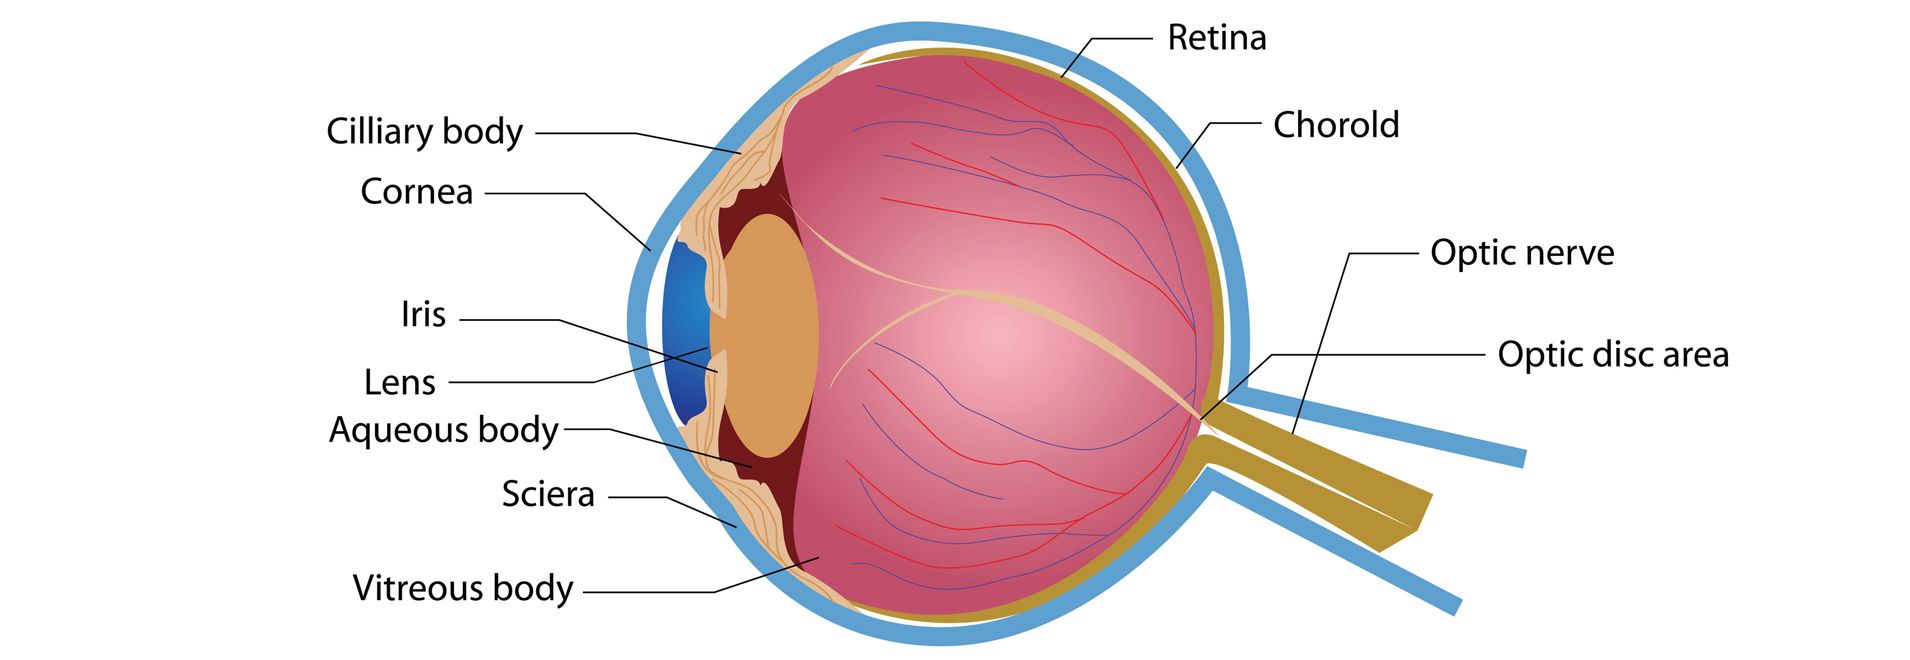
\includegraphics[width=0.8\textwidth]{./images/anatomy-of-the-eye.jpg}
    \caption{Anatomy of the eye \cite{eyeanatomy-pic}}
    \label{fig:eye-anatomy}
\end{figure}

The area of interest of this project is limited to the posterior segment of the eyeball as the tissues therein are of significant clinical value to ophthalmologists in the analysis and diagnosis of refractive errors (myopia) and ocular diseases (glaucoma) \cite{Ronchetti2017}. In particular, we will focus on the vitreous body, retina, choroid and sclera as they will form part of the set of the manually annotated scans used in our project. 

The vitreous body is an structure characterized by a colorless and transparent gel. It consists mainly of water and other aminoacids, proteins, salts and acids. The vitreous is located between the lens and the retina and occupies 4/5 of the total volume of the eye. It serves mainly to transmit light from the lens to the retina and is also believed to contribute to the convergence power of the eye \cite{snell1998}. 

Once the light has traveled through the vitreous body, it reaches the retina, a layer of nervous tissue that covers the inside of the back two-thirds of the eyeball envolving the vitreous. As a part of the central nervous system, the retina converts light waves detected by its photoreceptors into electric signals that travel to the brain via the optic nerve \cite{purves2001}. In other terms, it converts light into electric signals that are sent to the brain and interpreted there as images.

Due to its vascular structure, the choroid\textquotesingle s irrigates the outer retina with oxigen through an intrinsic layer of capillaries   \cite{snell1998, choroidExpl}. Several studies \cite{Ronchetti2019, Ronchetti2018} indicate that choroidal thickness could be correlated with the development and progression of myopia and various ocular diseases. 

Finally, the sclera protects the inner part of the ocular globe through its collagenous structure. Together with the cornea, it serves to contain the internal pressure of the eye and also the forces created by the external muscles of the eye during eye movement \cite{Meek2008}.

\section{Technical Background}\label{s:TechBack}


\subsection{Optical Coherence Tomography}
Optical Coherence Tomography (OCT) is the standard technique for producing accurate visualizations of ophthalmic medical images \cite{Garrido2014}. Since OCT uses near-infrared low-coherence light waves to produce measurements of the reflectivity vs. depth (also known as A-scans\cite{Garrido2014}) it represents a non-invasive procedure to extract information from the ocular globe structure. Several A-scans from consecutive zones can be combined in order to form a 2D image of the posterior segment of the eye where the vitreous, retina, choroid and sclera can be clearly located. Finally, a contiguous set of B-scans produces a volumetric image that ophtalmologist can use to first evaluate the retinal and choroidal structure and second calculate the layers thickness and issue diagnoses on several type of diseases including various ocular diseases \cite{Ronchetti2019}, Diabetes \cite{Jiang2018}, Alzheimer, Glaucoma and other neurodegenerative diseases \cite{DENHAAN2017162}.   


\begin{figure}[H]
    \centering
    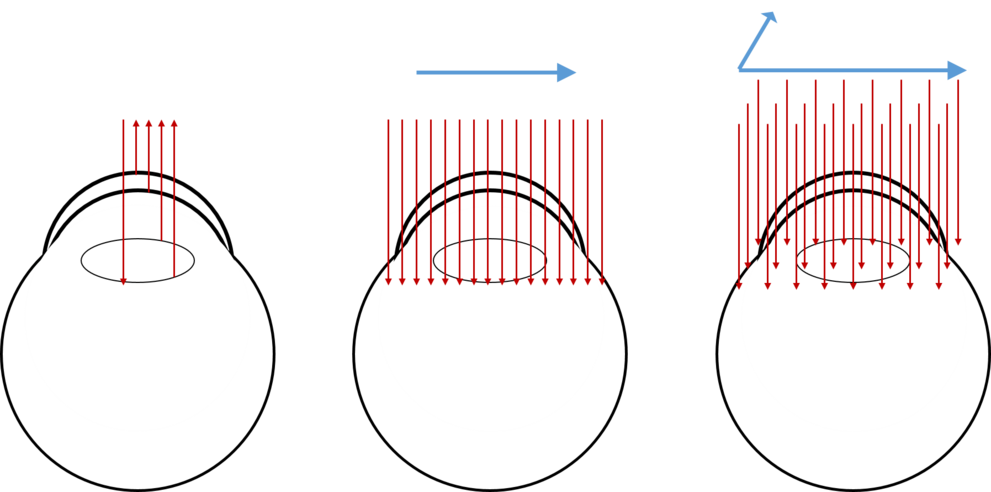
\includegraphics[width=0.8\textwidth]{./images/csm_ABC_scans.png}
    \caption{Scan Types in Optical Coherence Tomography \cite{Willdeman2016}. From left to right: A-scan use a signal depth profile composed of time-gates reflections; B-scan use a frame composed of array of A-scans; Volume use a 3D dataset composed of array of B-scans.}
    \label{fig:mb-oct-abcscans}
\end{figure}

As stated in the motivation of this thesis, retinal and choroidal thickness can be measured from OCT scans with the help of annotated ground truths establishing the locations of the tissues\textquotesingle boundaries. In the case of the retina, the Internal Limiting Membrane (ILM) divides it from Vitreous on the upper boundary \cite{MACNAIR2015343}, while the Bruchs Membrane (BM) divides the retina from the choroid \cite{BOOIJ20101} serving as the retina's bottom boundary. Subsequently, the Choroidal-Scleral Interface separates the choroid from the sclera \cite{Ronchetti2018}. The mentioned boundaries create a segmentation map within OCT B-Scans where the vitreous body, retina, choroid and sclera can be analysed as presented in Fig.~\ref{fig:annotated-oct-scan}. 


\begin{figure}[H]
    \centering
    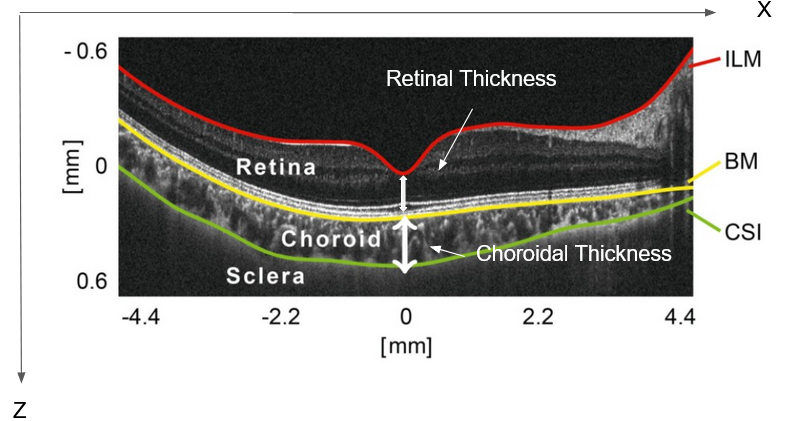
\includegraphics[width=0.8\textwidth]{./images/OCT-Scan.png}
    \caption{A B-scan with segmented layers from top to bottom:  Internal Limiting Membrane (ILM),  Bruch's Membrane (BM), Choroid-Sclera Interface (CSI) \cite{Ronchetti2019}}
    \label{fig:annotated-oct-scan}
\end{figure}

\subsection{Convolutional Neural Networks}\label{s:cnn}

A CNN is a powerful family of neural networks inspired by biological processes and containing Convolutional Layers, used in the field of deep learning. The design of the connection pattern is inspired by the structure of the neurons in the visual cortex of animals. Modern CNNs are effective for obtaining accurate models, as they require fewer parameters than fully connected architectures, and are often computationally more efficient because convolutions can be easily parallelized on GPU cores \cite{DIDLBook}. Furthermore, CNN-based architectures are widely used in the computer vision field, as they are prized for their efficiency. 

To be functional, Convolutional Networks require some operations; capturing features from images is achieved by applying a set of operations known as convolution and pooling, which are described in this chapter. 

If you want to process datasets by collecting and annotating pixels of images, you can quickly end up with a network that has huge dimensions, which leads to poor GPU performance. For this reason CNNs are used for data that is not tabular\footnote{By ``tabular'' we mean data consisting of rows corresponding to samples and columns corresponding to features.} \cite{DIDLBook}. The main role of the CNN is to facilitate the processing of images by reducing them to a form that is easier to examine without losing the features that are essential for good prediction.

\subsubsection{Convolution Operation}
An important concept of CNN is spatial invariance\footnote{Spatial invariance refers to the invariance of the model towards spatial transformations of images such as rotation, translation and scaling.}, which refers to the ability of a CNN model to recognize and identify features even when the input is transformed or slightly modified. In other words, object recognition is not sensitive with respect to their exact position in the image. In computer vision, adding convolution to the neural network allows the addition of an inductive visual prior whereby objects can appear anywhere. Sharing the weights over the location of the object significantly reduces the number of parameters to be learned, the convolution is shifted when the object changes its position \cite{CNNSpatialLocation}. The earliest layers of our network should be implementing translation invariance, i.e., it should respond similarly regardless of where objects appears in the image. In addition, they should focus on local regions (``locality principle'') without regard to the content of the image in distant regions \cite{DIDLBook}.

The translation invariance implies that a shift in the input \(x\) should lead to a shift in the hidden representation \(H\) (i.e.~matrices in mathematics and two-dimensional tensors in code). 
This is a convolution as the weighting pixels at \((i + a, j + b)\) in the vicinity of location
\((i, j)\) with coefficients \([V]_{a,b}\) to obtain the value \([H]_{i,j}\): 
\begin{equation}
\label{eqn:invariance}
[H]_{i,j} = u + \sum_a\sum_b[V]_{a,b}[X]_{i+a,j+b}
\end{equation}
Note that X and H have the same shape while \([X]_{i,j}\) and \([H]_{i,j}\) denote the pixel at location \((i, j)\) in the input image and hidden representation. The translation invariance is only possible if V and u do not depend on \((i, j)\) \cite{DIDLBook}.
According to the aforementioned locality principle, it should not be necessary to look far away from the location \((i, j)\) to get information about what is happening in \([H]_{i,j}\). Outside a certain range \(|a| > \Delta \) or \(|b| > \Delta\), we should set  \([V]_{a,b} = 0\) and rewrite \([H]_{i,j}\) as follows \cite{DIDLBook}:
\begin{equation}
\label{eqn:locality}
[H]_{i,j} = u + \sum_{a=-\Delta}^{\Delta}\sum_{b=-\Delta}^{\Delta}[V]_{a,b}[X]_{i+a,j+b}
\end{equation}
The operations that provide spatial invariance (\ref{eqn:invariance}) and locality (\ref{eqn:locality}) are convolutions. In mathematics the convolution between two function \(f\) and \(g\) with \({ I\!R}^d \rightarrow { I\!R}\) is defined as follows \cite{DIDLBook}: 
\begin{equation}
(f*g)(x) = \int f(z)g(x-z)dz
\end{equation}
In other words, the convolution measures the overlap between \(f\) and \(g\) when one of the functions is “flipped” and shifted by \(x\). If we use two-dimensional tensors, we have a corresponding sum with indices \((a, b)\) for \(f\) and \((i-a, j-b)\) for \(g\), which is very similar to \ref{eqn:locality} (with the exception of using \((i+a, j+b)\) instead) \cite{DIDLBook}:
\begin{equation}
(f*g)(i,j) = \sum_{a}\sum_{b} f(a,b)g(i-a,j-b)
\end{equation}

\subsubsection{Pooling Operation}
In general, when processing images, it is more efficient to progressively reduce the detail of an image (for a given dimension) of our hidden representations. Thus, the higher one goes in the network, the larger the field of perception becomes, so the more the perceived image is composed of generalities rather than details. The final task we want to perform is, in the case of this work, a global one: to find out where the borderlines between the ILM, the BM and the CSI is. Therefore, the layers of our network should be sensitive to all the inputs in order to have a global view, this can be achieved by gradually accepting data and generating coarser maps but keeping all the advantages of convolutional layers at the intermediate processing layers. As with edge detection,  our representation must be invariant to translation, since changing just one pixel can change the image significantly. This is why pooling layers are used, which have the dual purpose of mitigating the location sensitivity of convolutional layers and spatially downsampling the representations. There are several types of (deterministic) pooling operations, here we discuss max-pooling and average-pooling \cite{DFTPooling}. Like convolutional layers, pooling operators operate on a fixed-size-window that moves through the different regions according to their step size \cite{DIDLBook}.
An example found in \cite{DIDLBook} shows how these operators work. If we take a 3$\times$3 matrix representing our input and imagine that the operator from the upper left corner from left to right and up and down, a max-pooling operation will create a new 2$\times$2 matrix: 

\begin{figure}[H]
    \centering
    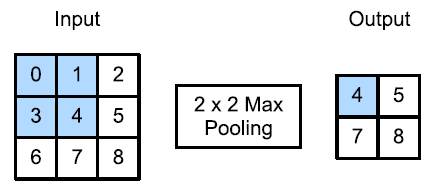
\includegraphics[width=0.8\textwidth]{./images/pooling_example.png}
    \caption{Pooling Operation example  \cite{DIDLBook}}
\end{figure}
Basically the max-pooling operation is to take the max value of a part of matrix (left blue) and place it in a new matrix (right) and then move and repeat this possess until the new matrix is populated.
\[max(0, 1, 3, 4) = 4,\]
\[max(1, 2, 4, 5) = 5,\]
\[max(3, 4, 6, 7) = 7,\]
\[max(4, 5, 7, 8) = 8.\]


as well as average -pooling would have given:
\[average (0, 1, 3, 4) = 2,\]
\[average (1, 2, 4, 5) = 3,\]
\[average (3, 4, 6, 7) = 5,\]
\[average (4, 5, 7, 8) = 6.\]

\subsubsection{Softmax Operation}\label{tech:softmax}
The softmax function is a logistic function generalized to multiple dimensions and is used as an activation function for neural networks. It is used to normalize the input vector z of K real numbers to a distribution consisting of K probabilities over predicted output classes. In this project we have four classes (vitreous, retina, choroid, sclera), therefore using softmax is relevant since it is a classifier which has excellent performance for multi-classification tasks and will often be used as the final layer of the network \cite{SoftMaxClassification}. 
The traditional softmax classifier can be described as follow: let  K be the number of classes, \(z_i\) we obtain  label and \(z_j\) the j-the element of the vector of class scores \cite{SoftMaxClassification, DIDLBook} :

\begin{equation}
\sigma(z_{ij}) = \frac{e^{z_i}}{\sum_{j=1}^{K} e^{z_j}}
\end{equation}
Once the convolution and pooling function have repeated until we have a pixel to be classified, the softmax function is used to determine the probability that this pixel belong to a certain class.

\subsection{U-net}\label{tech:unet}

U-net is a CNN architecture developed for the field of biological images where samples are scarce and the outputs involve assigning certain regions of the image to one or more classes. Previously, an sliding window was the standard method to perform this task, but the method is computationally expensive and requires an enormous amount of time depending on the image dimensions \cite{Ronneberger2015}. Therefore, in 2015 Prof. Dr. Olaf Ronneberger from the University of Freiburg in Germany developed an architecture consisting first of a contracting or encoding path that uses a combination of convolutional and pooling operations in order to aggregate and classify pixels. Once the pixel has been recognized the architecture proposes a second expansive path using up-sampling operations where the classified pixels are concatenated with features from the contracting or decoding path to add localization information. 

\begin{figure}[H]
    \centering
    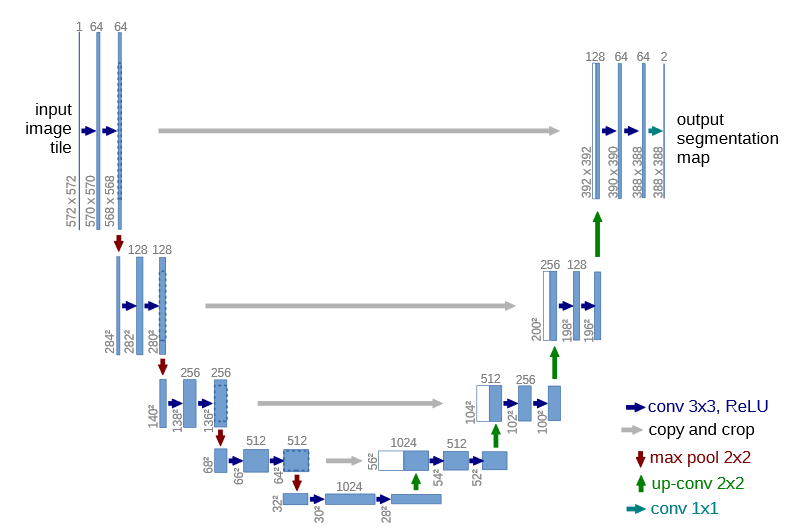
\includegraphics[width=0.8\textwidth]{./images/Unet-architecture.png}
    \caption{U-net architecture \cite{Ronneberger2015}. The blue boxes represent multichannel feature maps while the arrows represent the different mathematical operations described in Sec. \ref{s:cnn}    }
\end{figure}

The architecture is faster and less expensive than sliding windows since pixel features are aggregated to avoid classifying them individually. The second most important contribution of the paper is the idea of using image augmentation to circumvent the problem of image scarcity. By augmenting the image dataset, we apply a series of common image transformation operations in order to slightly modify the base image and create synthetic copies that reinforce learning. The detail of these operations is explained in Sec. \ref{ss:datapreparation}.

\section{Previous Work}\label{s:prevWork}
\subsection{Computer Vision Methods for Detection of Early Choroidal Thickness Changes in Myopic Asian School Children}

Computer vision methods for the automated segmentation of inner retinal and choroidal layers obtained from optical coherence tomography (OCT) imaging \cite{Ronchetti2019statistic} can be used to generate a reliable set of annotated scans. 
The contribution of this project lies in the documentation and explanation of the most frequent methods used for measuring retinal thickness from an algorithmic perspective to provide a framework to easily extract features from OCT B-scans. 
There are several approaches for detecting retinal boundaries in OCT B-scans, among them we can cite pixel intensity variations, texture analysis and graph search-based segmentation techniques. Pixel intensity variations are often used when calculating the total retinal thickness \cite{Alonso-Caneiro2013}, the method involves a series of computer graphic processing steps where each pixel of the image is compared to a threshold chosen according to the color intensity of the pixels that contain the information about the location of the boundary \cite{Fabritius:09}. 
\\
In the case of the ILM, it can be easily extracted because the lens pixels in the OCT scans are mostly black while the membrane's pixels are mostly white, this is mainly due to the density of the element, the more dense the element is, the whiter it will appear in the image \cite{Brar597}. Therefore, taking the image from the top left corner, one can run a search algorithm that finds the first white pixel \footnote{The first pixel that is over the threshold} from top to bottom and return its position. Running this same algorithm across the $x$ axis produces us an array of pixels that can be smoothed by using cubic-spline interpolations that corresponds to the ILM. The process for extracting the BM inner-most layer is the same, since the sclera presents opaque pixels that can be omitted by the algorithm, the process would start from the bottom left corner and runs the algorithm from bottom to top searching white pixels until it reaches the BM. The CSI is ignored in this works since the choroid’s boundary with the sclera is way too hard to identify using pixel intensity variation. 
The retinal thickness was also computed to output an average thickness and an average thickness in 5 zones, producing the following image:

\begin{figure}[H]
    \centering
    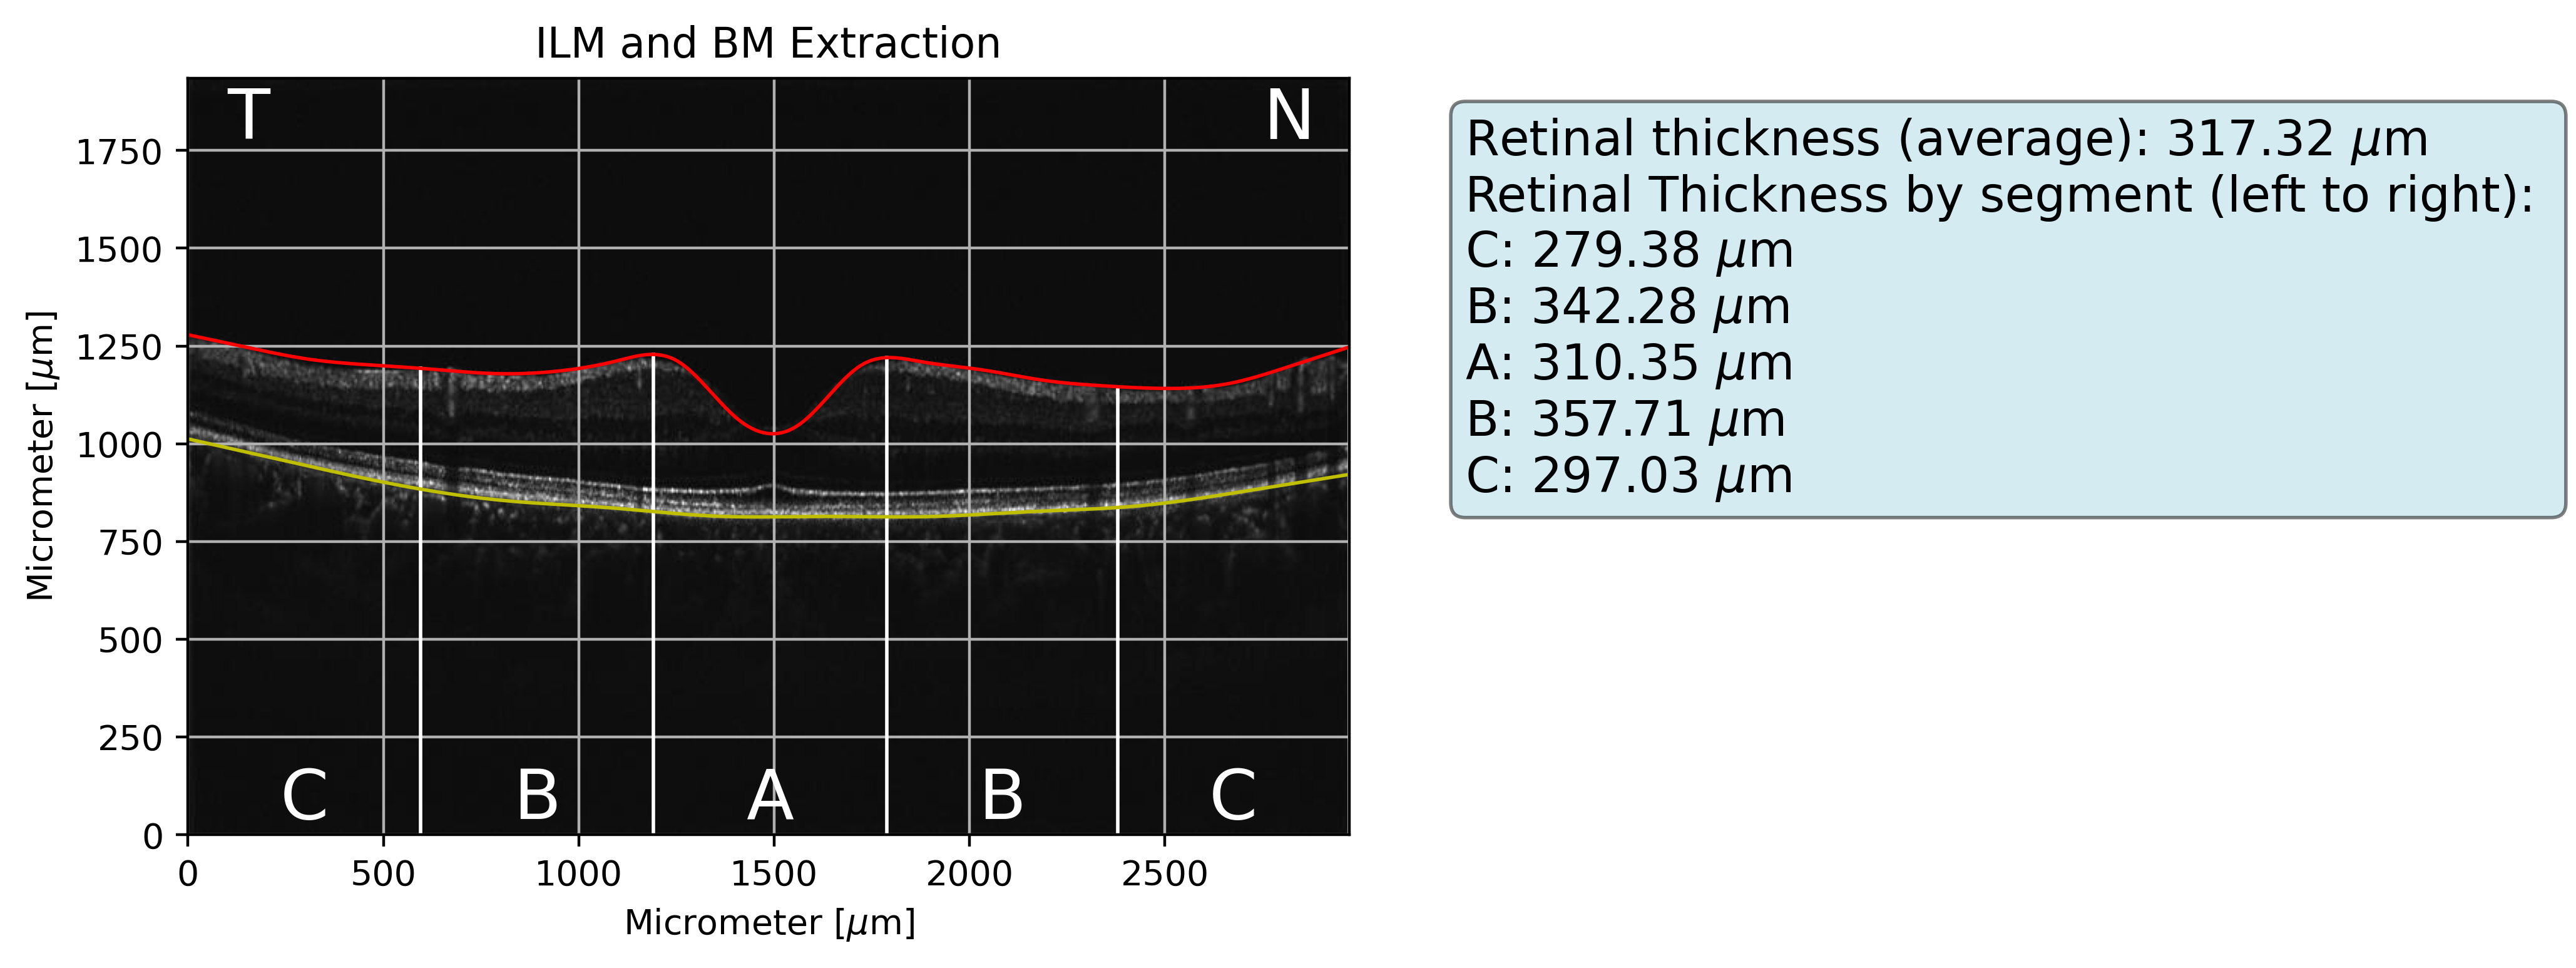
\includegraphics[width=1\textwidth]{./images/ILM_BM_Extracted.png}
    \caption{Final rendering of the ILM, BM and retina thinckness}
    \label{fig:final_rendering}
\end{figure}

During this study, it has been confirmed that OCT scan quality can greatly impact the result of an automated solution and potentially break the smoothing algorithm in the post-processing phase. When the scan had too much artefact it was almost impossible for the algorithm to correctly identify the ILM or the BM. Using this method only might result in a solution that cannot be fully automated, thus other methods like graph-based search must be explored. In this case, adjusting the natural smoothing spline parameter can improve the accuracy of the detected boundaries, but only in certain cases which fully depend on the OCT scans. To automate the process of generating annotations for a machine learning model, either a manual approach or a semi-automated solution might produce better results that are more accurate to the actual membrane's position.  

\subsection{Literature Review}
There have been efforts to automate OCT scan segmentation using deep learning methods, although one of its principal limitations is described in Ronchetti et al. \cite{Ronchetti2019} and Alonso-Caneiro et al. \cite{Alonso-Caneiro2013} as a low degree of interannotator agreement when detecting the CSI, which would introduce significant differences in the class segmentation and consequently would lead to inconsistencies in choroidal and retinal thickness measurements. Moreover, it has been shown in \cite{Maloca2021} that the performance of deep learning methods is at it's best an average of the experts' annotations.

In 2017, Roy et al. \cite{Roy2017} proposed a fully convolutional deep learning architecture to segment retinal layers and fluid masses in OCT scans called ReLayNet. The architecture is used to train a joint loss function composed by  a weighted logistic regression and a Dice overlap. It proposes a similar encoder-decoder architecture using convolutional and pooling operations and additionally adding a softmax operation block for classifying pixels.

\begin{figure}[H]
    \centering
    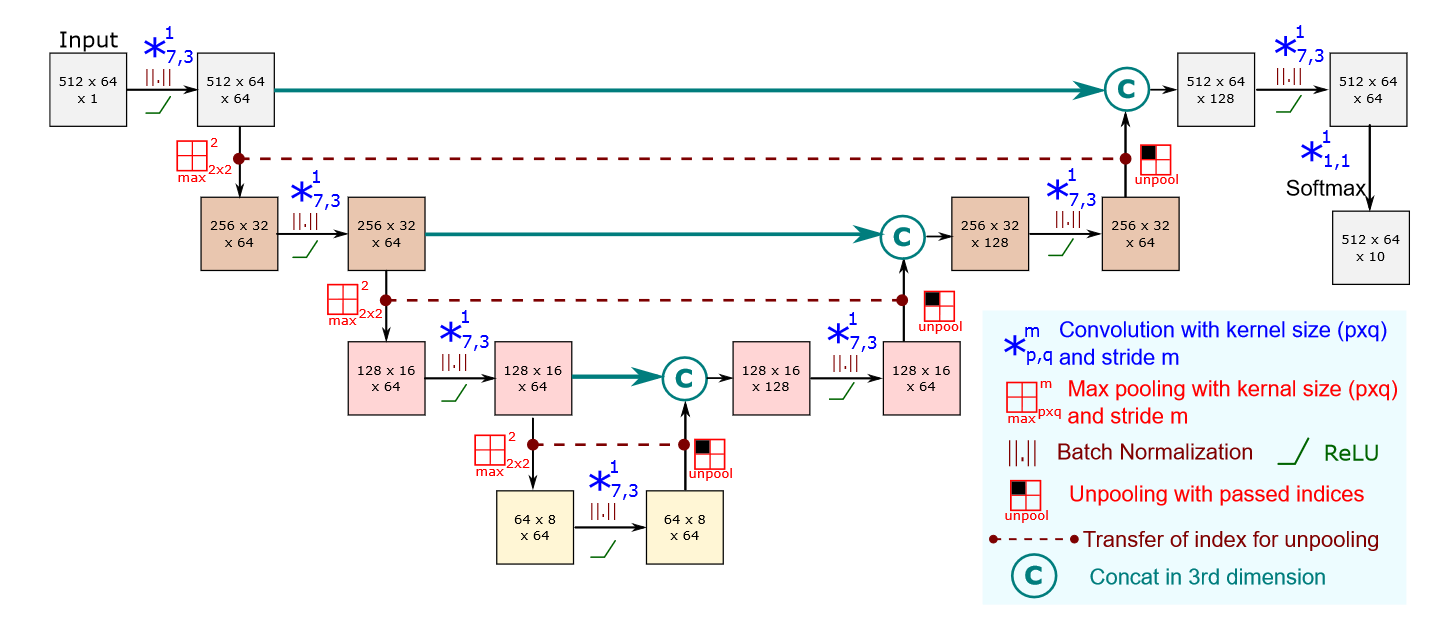
\includegraphics[width=0.8\textwidth]{./images/relaynet-architecture.png}
    \caption{ReLaynet architecture \cite{Roy2017}.}
\end{figure}

The model was trained in a dataset composed by 110 OCT B-scans of size 512*740 pixels annotated by two expert ophtalmologists. Using a 8-fold cross validation method, the results indicate a higher dice overlap score against other common used methods as U-net or FCN.

\begin{figure}[H]
    \centering
    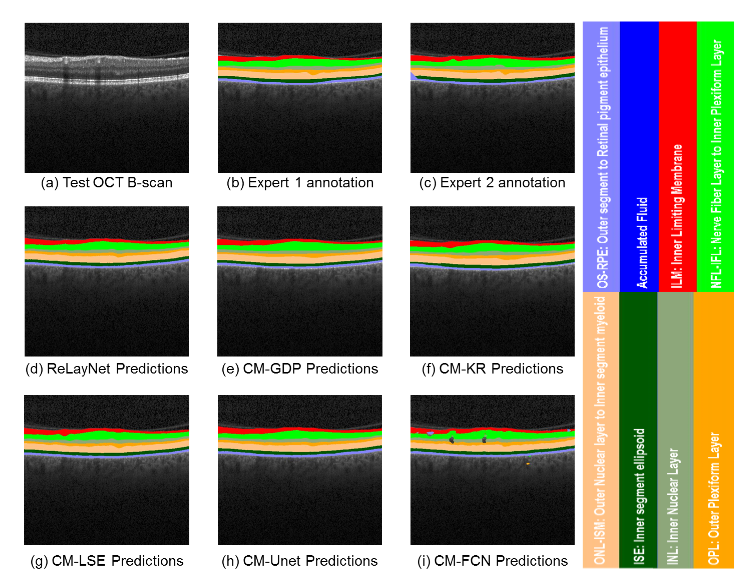
\includegraphics[width=0.8\textwidth]{./images/relaynet-predictions.png}
    \caption{OCT B-scan predictions using ReLaynet architecture model. In average the proposed model had a ILM's dice overlap score of 0.90 against U-net's 0.86 and 0,87 for the model known as Layer specific structured edge learning with  Graph based dynamic programming  \cite{Roy2017}.}
\end{figure}

Maloca et al. \cite{Maloca2019} validated the usage of deep learning methods by implementing a U-net CNN trained on a dataset of 2070 B-scans. The data was annotated manually by segmenting 4 compartments corresponding to the vitreous, retina, choroid and sclera. This was performed by identifying the ILM, the choriocapillaris (CC) and CSI. In this work the use of the choriocapillaris was preferred due to the thinness of the BM in OCT scans which makes it unrecognizable.

\begin{figure}[H]
    \centering
    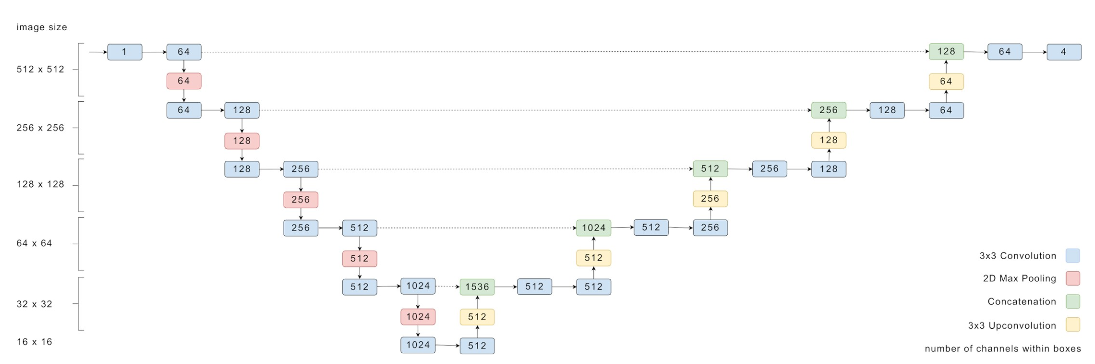
\includegraphics[width=0.8\textwidth]{./images/maloca-unet.png}
    \caption{Depiction of the U-net model used in \cite{Maloca2019}}
\end{figure}

The metric used to measure the performance of the U-net model in \cite{Maloca2019} was the Intersection over Union (IoC) also known as Jaccard coefficient, where all the matching pixels between both images are divided between the total of pixels of both images, giving a clear measure of similarity between both images. The results indicate mean IoU scores of 0.9929 for vitreous, 0.9690 for retina, 0.8819 for choroid and 0.9768 for sclera when benchmarked to a validation dataset of 60 images. From these results the authors concluded that the outputs of the proposed CNN were on par with manual segmentations made by human experts.

\begin{figure}[H]
    \centering
    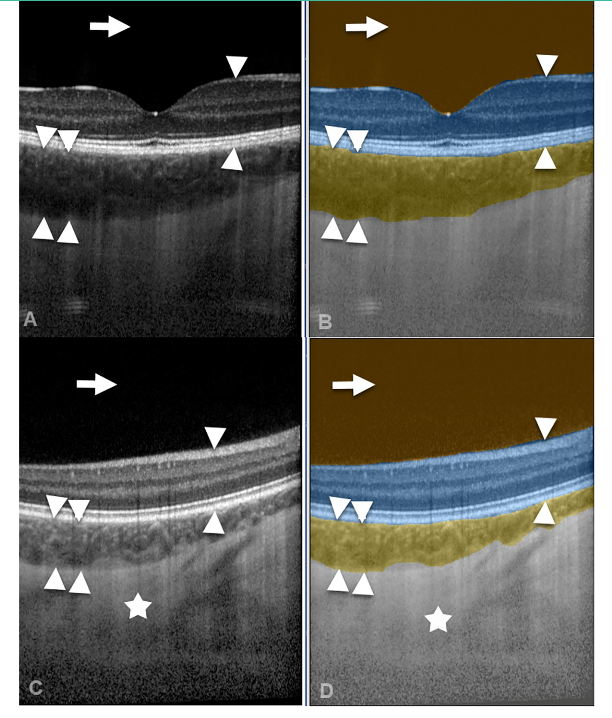
\includegraphics[width=0.7\textwidth]{./images/maloca-segmentations-results.png}
    \caption{Illustration of the predictions made by Maloca et al. A spectral-domain OCT image (A) and a swept-source OCT image (C) were automatically segmented by the CNN (B,D) in to the compartments vitreous (arrow), retina (arrowheads), choroid (double arrow heads), and sclera (asterisk) \cite{Maloca2019}.}
\end{figure}


Zheng et al. \cite{Zheng2020} proposed using a modified U-net architecture for automated segmentation of the choroid based on the Residual U-net model (ResNet) \cite{He2015} achieving higher performance with fewer parameters by using layers of residual functions. 
\begin{figure}[H]
    \centering
    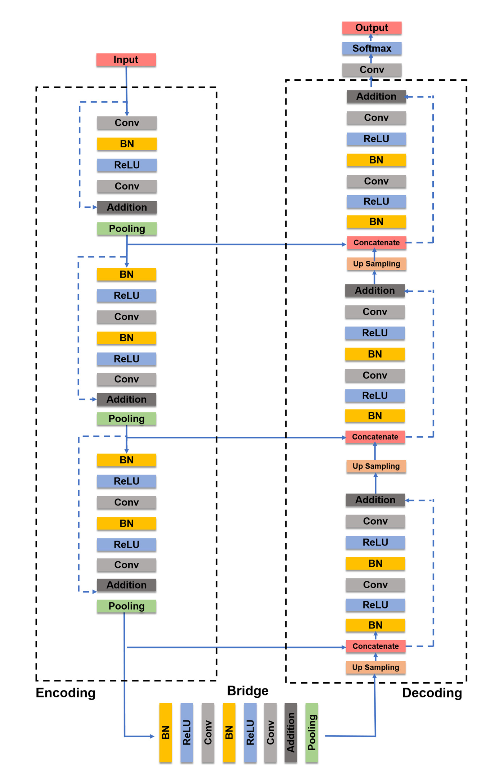
\includegraphics[width=0.6\textwidth]{./images/ResNet-architecture.png}
    \caption{Residual U-net model proposed by \cite{He2015} and used in \cite{Zheng2020}}
\end{figure}

The model was applied to a dataset composed by 450 OCT B-scans that were augmented to 1436 scans of 2048*1561 pixels. The performance was measured using the intraclass correlation coefficient (ICC) which is described as the level of resemblance between two or more samples of the belong to a common group defined by a particular set of characteristics. In Zheng's paper the compartments were conformed by choroidal boundaries Bruch's Membrane and Choroidal Scleral Interface and a set of vasculature measurements such as the choroidal vascularity index (CVI), choroidal stromal index (CSI), luminal area (LA) ,stromal area (SA), the total choroidal area (TCA),and Choroidal Thickness (CT). For the CT the ICC between human and automated samples was 0.994 with a CoV of 2.284.For the other For the parameters CVI, CSI, LA, SA, and TCA, the value of ICC were 0.966, 0.977, 0.977, 0.964, 0.994 with CoValues of 2.230, 3.277, 1.653, 5.024, and 2.284, respectively.

\begin{figure}[H]
    \centering
    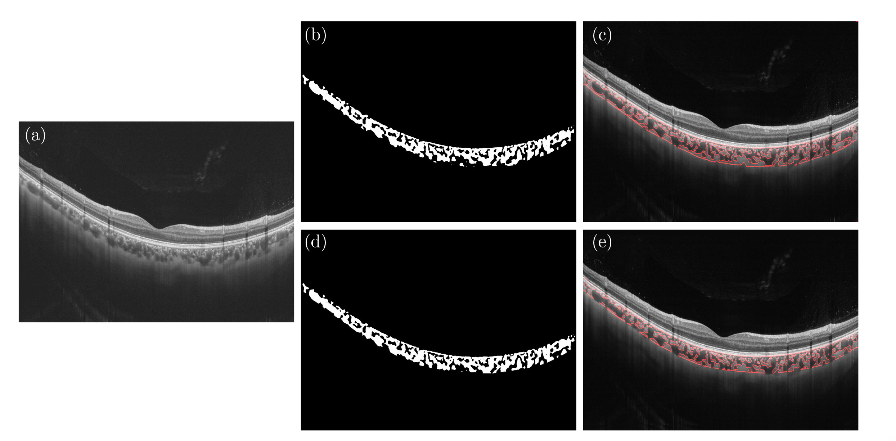
\includegraphics[width=0.8\textwidth]{./images/choroidal-segmentation-zheng.png}
    \caption{Predictions obtained by Zheng et al. (a) Raw OCT Scan (b) automatic identification of the upper and lower choroid boundaries; (c) binarization image of the choroid and (d) demarcation of luminal area (LA) and stromal area (SA) with red dotted line. \cite{Zheng2020}}
\end{figure}





\section{Discussion}\label{s:Discussion}

In this section, we will detail the process of creating the framework from its inception point to evaluating the final output. In order to standardize its description we have chosen to fit our process to the machine learning workflow. 

\subsection{Data Collection}\label{ss:data_collection}
For this project we used a dataset composed of 755 OCT B-scans\footnote{See Sec.~\ref{s:TechBack} for more details.} of 500$\times$768 pixels. The data was obtained from Asian patients in the age range of 8-18 years stemming from urban regions with a high prevalence of myopia. The subjects were healthy with globally good distance and near vision, no systemic and ocular diseases, ocular trauma or surgery \cite{Ronchetti2019}. The images were acquired by a dual-wavelength eye-tracking OCT system operating simultaneously at the 870 and \SI{1075}{\nano\metre} bands. This system was developed by the HuCE-optoLab of the Bern University of Applied Sciences in Biel, Switzerland under the supervision of Prof.~Christoph Meier and Dr.~Boris Pova\v{z}ay\cite{Ronchetti2019}  before it was transferred and setup at the Hong Kong Polytechnic University\textquotesingle s School of Optometry\footnote{For more information about the OCT dataset we refer the interest reader to \cite{Ronchetti2019}}.

\subsubsection{Data Annotation}

The scans were annotated by a group of 6 ophthalmologists recruited as experts. Using an online tool they were able to draw the ILM, BM and CSI boundaries in the OCT scans (see \cite{Ronchetti2019} for more details).

\subsubsection{Mask Segmentation}
On the set of annotated scans, we ran an algorithm to merge the three separate layers into a single image, as depicted in Fig.~\ref{fig:merged}

\begin{figure}[H]
    \centering
    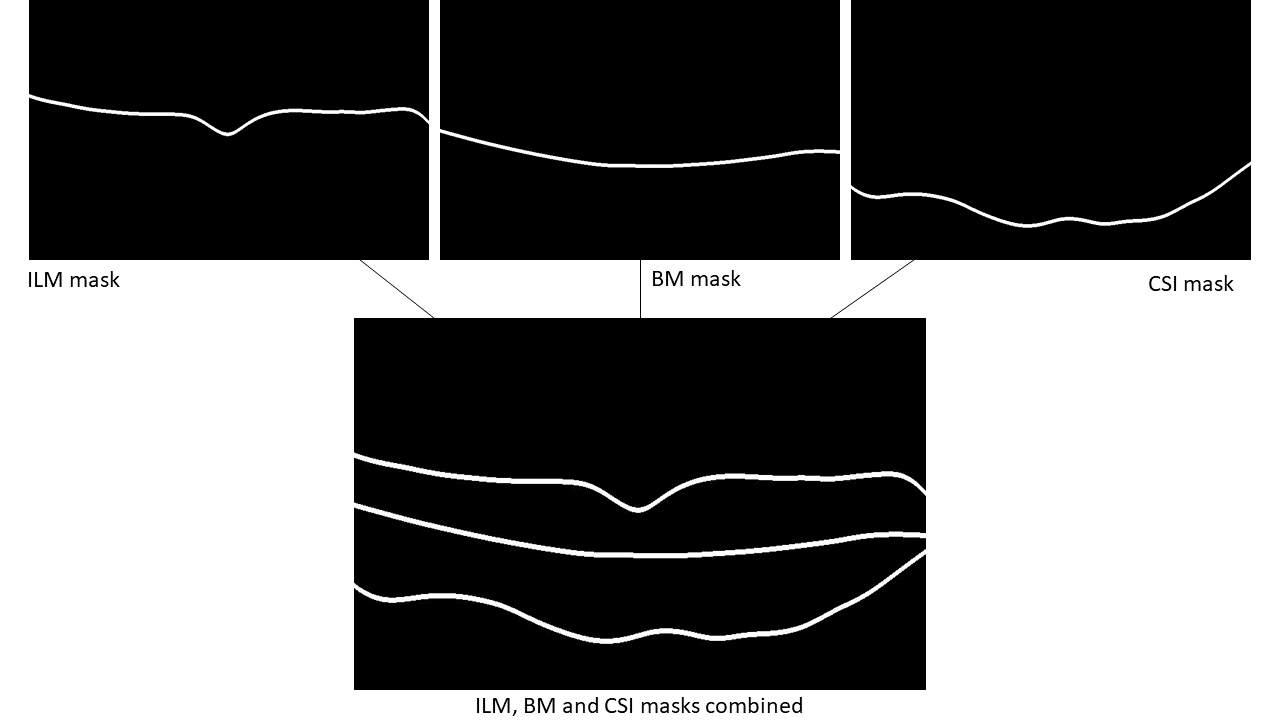
\includegraphics[width=1\textwidth]{./images/ILM_BM_CSI_merged.png}
    \caption{Merged ILM, BM, CSI Layers.}
    \label{fig:merged}
\end{figure}

As a next step, we assigned a specific value to each pixel in the 4 respective compartments, thus obtaining a segmentation map, in which we can clearly delineate the vitreous, retina, choroid and sclera. Because of artifacts in data acquisition and a different number of annotated samples for each of the layers, not all scans could be processed by our algorithm, so the dataset was reduced to a total of 755 fully segmented B-scans.

\begin{figure}[H]
    \centering
    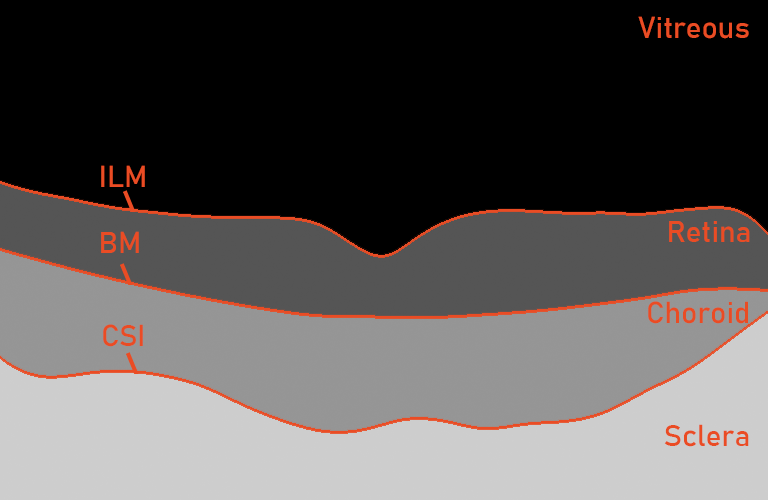
\includegraphics[width=0.7\textwidth]{./images/chun_w00_fix_14_segmented_annotated.png}
    \caption{Segmentation Map used for training. \emph{Note that red elements are not part of the segmentation mask but has been added for clarity in this image}}
    \label{fig:annotated-layers}
\end{figure}

\subsection{Data Preparation}\label{ss:datapreparation}
First we define a size for the images we will feed to our model with, here we chose the size 256$\times$256 as this is the default size of images used in Keras \cite{chollet2015keras}. Also, we could not work with images that have a high resolution, as this would cause memory overflow during the training of the model. The data can be loaded via the method \emph{load\_data()} defined as follows:
\begin{lstlisting}[caption=The method for loading data can be found in the \emph{helper.py} file]
def load_data(datapath, is_train_data):
    images = []
    for directory_path in glob.glob(datapath):
        for img_path in sorted(glob.glob(os.path.join(directory_path, "*.tif"))):
            img = cv2.imread(img_path, 0)  # Read image as gray scale  
            zeros = np.zeros([config.IMAGES['IMG_SIZE_X']-config.IMAGES['IMG_SIZE_Y'], config.IMAGES['IMG_SIZE_X']]) 
            img = np.concatenate((zeros, img)) # Squaring the 500*768image to 768*768
            if(is_train_data):
                img = cv2.resize(img, (config.IMAGES['IMG_SIZE_TRAIN_Y'], config.IMAGES['IMG_SIZE_TRAIN_X']))
            else:
                img = cv2.resize(img, (config.IMAGES['IMG_SIZE_TRAIN_Y'], config.IMAGES['IMG_SIZE_TRAIN_X']), interpolation = cv2.INTER_NEAREST)  #Otherwise 
            images.append(img)
    #Convert list to array for machine learning processing        
    images = np.array(images)
    
    return images
\end{lstlisting}

We use \emph{LabelEncoder} \cite{scikit-learn} to encode our label with a value between 0 and n-classes-1, where n is the number of distinct labels, here we have four: the vitreous, retina, choroid and sclera. This allows us to add a weight to each of our classes and help to reduce class imbalance in our model. By ``class imbalance'' we mean that not all our classes have the same number of pixels; consequently, this can lead to bias in the model. If we look at the segmentation map in Fig.~\ref{fig:annotated-layers}, we can see that the vitreous covers much more pixels than the retina. Therefore, to achieve good performance, the model might tend to focus more on the vitreous pixels. So if one class has more pixels than another, it means that it has a higher weight in the model accuracy results than another because it has a higher percentage of pixels in the image. The goal is to balance the weighting of the classes to avoid this kind of situation which could lead to a biased model. To achieve this, we use the \emph{'balanced'} parameter of the \emph{sklearn} \cite{scikit-learn} \emph{compute\_class\_weight} method which automatically compute the weights using a logistic regression based algorithm \cite{scikit-learn} to balance our dataset. 

\begin{lstlisting}[caption={Encoding of the labels and weights attributions to the class, code from \emph{train.py} file}]
from sklearn.preprocessing import LabelEncoder
labelencoder = LabelEncoder()
n, h, w = train_masks.shape
train_masks_reshaped = train_masks.reshape(-1,1)
train_masks_reshaped_encoded = labelencoder.fit_transform(train_masks_reshaped)
train_masks_encoded_original_shape = train_masks_reshaped_encoded.reshape(n, h, w)

np.unique(train_masks_encoded_original_shape)

from sklearn.utils import class_weight

class_weights = class_weight.compute_class_weight(
                    'balanced',
                     np.unique(train_masks_reshaped_encoded),
                     train_masks_reshaped_encoded)
\end{lstlisting}

Normalization of a vector in mathematics means dividing the vector by its norm \cite{Normalization_Vector_Machines:2001}. In other words, the idea is to make the Euclidean length of the vector equal to one. In neural networks, normalization is important to obtain good results and reduce the calculation time \cite{Normalizazion_NN}, and usually means re-scaling by the minimum and range of the vector, to make all the elements lie between 0 and 1. Normalisation is not a requirement for multi-layer perceptron but we still opted for it because our activation function, softmax (see sec. \ref{tech:softmax}), has a range of [0,1] and we therefore want to ensure that our target values lie within that range.

\begin{lstlisting}[caption={Normalize the data, the code can be found in the \emph{train.py} file}]
#Normalize Data
train_images = np.expand_dims(train_images, axis=3)
train_images = normalize(train_images, axis=1)

train_masks_input = np.expand_dims(train_masks, axis=3)
\end{lstlisting}

We can now split our data-set in two parts, one for the training and one for testing. We do this as a means of estimating classification accuracy \cite{DatasetSplitting:2011}. We chose to split that data-set in a 80\%-20\% \footnote{80\% of the images for the training set and the remaining 20\% for the testing set} proportion, as we don't have a a huge dataset we wanted to keep most of it for the training of the model.
\begin{lstlisting}[caption={Dataset split for testing and training from the \emph{train.py} file}, label={lst:data-split}]
# Picking 20% for testing and remaining for training
from sklearn.model_selection import train_test_split
x_train, x_test, y_train, y_test = train_test_split(train_images, train_masks_input, test_size = 0.20, random_state = 0) 
\end{lstlisting}

Then we need to encode our label from categorical features to their numeric representation, as it is required for neural networks. We use \emph{to\_categorical} from Keras \cite{chollet2015keras} to convert our current class vector to its binary matrix representation.

\begin{lstlisting}[caption={Data conversion into categorical, code belongs in the \emph{train.py} file}, label={lst:data-categorical}]
from keras.utils import to_categorical
train_masks_cat = to_categorical(y_train, num_classes=n_classes)
y_train_cat = train_masks_cat.reshape((y_train.shape[0], y_train.shape[1], y_train.shape[2], n_classes))
\end{lstlisting}

Usually deep learning requires a large volume of data to have good performances, but as we saw in Sec. \ref{Methodology:data} we only have 755 OCT B-scans. We already use U-net (Sec.~\ref{tech:unet}) to overcome this problem because it was specially designed for small dataset usage, one top of that data augmentation can be added to artificially increase the number of data we feed to the model. Data augmentation is a widely adopted approach for increasing the amount of training data \cite{AugAndEval:2017} but it could be at the expense of a loss of quality as too harsh modifications lead to loss of information in the data. This is even more true in our case because the OCT B-scans are presuppose nanometer precision (see Sec. \ref{Methodology:data}), we therefore want to be cautious in the choice of augmentation parameters.
We chose a rotation of maximum 5 degrees because after some testing we realized that more rotation would lead to too much loss on the borders of the images and as the scan are usually similarly in the spatial positioning of the layers it would mislead the model. The \emph{"reflect" fill-mode} to obtain a more consistent result to replace missing part of the images. We use an elastic function to compute the distortion, the function creates random displacement fields for height and width and smoothing the fields with a Gaussian. 
\begin{lstlisting}[caption={Base generator for image augmentation, the definition of the 2 seperate generator (image and mask) can be found in \emph{train.py}}]
train_datagen= ImageDataGenerator(rotation_range=5,
    fill_mode="reflect",
    shear_range=5,
    preprocessing_function=lambda x: elastic_transform(x, alpha_range=10, sigma=5)
)
\end{lstlisting}

We use data generator to real-time data feed our Keras model with augmented data. Using data generator also means that if the dataset we use is to grow in the future we avoid the problem of having dataset that are memory consuming to load.


\subsection{Model Development}

We based our model on the U-net architecture due to its flexibility to adapt to different types of images. We used a combination of an implementation made by Dr. Ronchetti (as part of a side project by \cite{Ronchetti2019}) and the youtuber DigitalSreeni \cite{DigitalSreeni}.

According to the original U-net model, the contracting path is a combination of convolution and pooling operations as illustrated in Fig. \ref{fig:model}.

\begin{figure}[H]
    \centering
    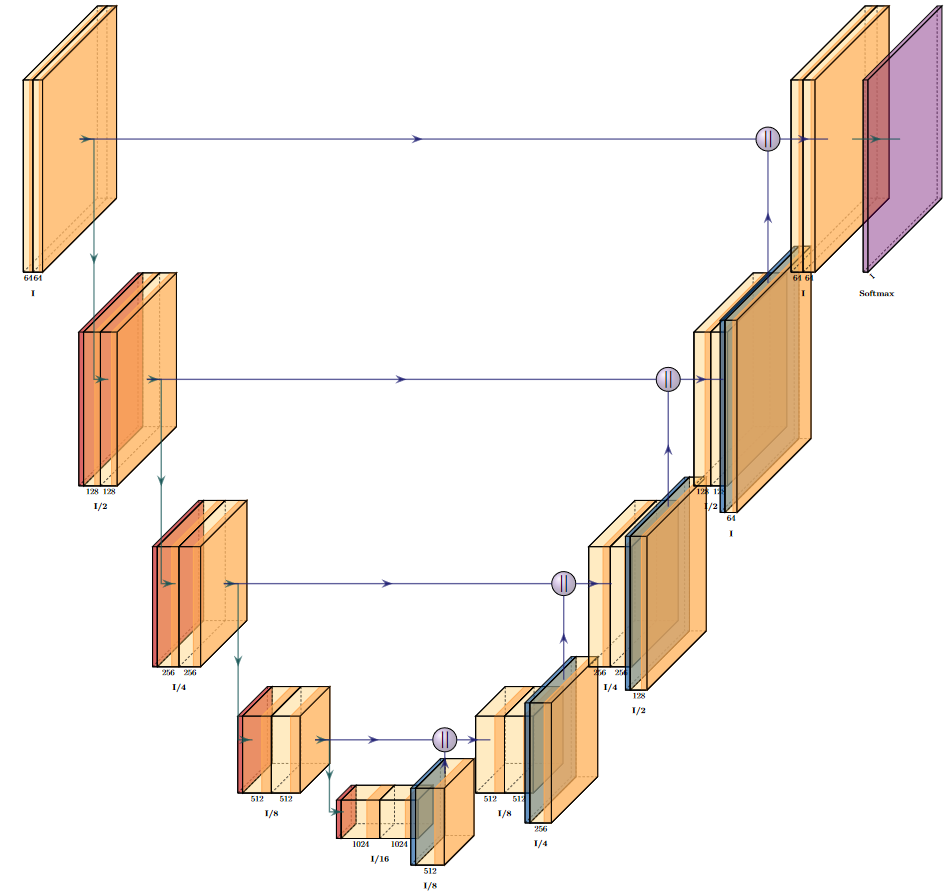
\includegraphics[width=\textwidth]{./images/U-net_ThesisVersion.png}
    \caption{Model implementation based on U-net}
    \label{fig:model}
\end{figure}

Our first convolutional layer has 64 filters as described in Lst. \ref{lst:conv2D-1}, we use a 3x3 kernel initialized by the keras initializer \emph{he\_normal} which draws samples from a truncated normal distribution centered on 0 with $stddev = sqrt(2 / fan\_in)$ where \emph{fan\_in} is the number of input units in the weight tensor. The layer uses the same padding to avoid the loss of data information and the activation function is the Rectified Linear Unit (relu) which fires the neuron for every positive value resulting from the convolution. 

It's important to mention that in order to avoid overfitting we drop 10\% out of the output data that runs through the network and finally we apply a pooling operation with a 2x2 kernel size in order to propagate the pixels with the most important features to the next neuronal layers.

\begin{lstlisting}[caption={Implementation of the first level of the contracting path, the rest of the layer can be found in the \emph{get\_unet()} method from \emph{model.py}}, label={lst:conv2D-1}]
inputs = Input((img_rows=256, img_cols=256,1))

c1 = Conv2D(filters=64, kernel_size=(3, 3), activation='relu', kernel_initializer='he_normal', padding='same')(inputs)
c1 = Dropout(0.1)(c1)
c1 = Conv2D(filters=64, kernel_size= (3, 3), activation='relu', kernel_initializer='he_normal', padding='same')(c1)
p1 = MaxPooling2D((2, 2))(c1)
\end{lstlisting}

The decoder part of the model is presented in Lst. \ref{lst:conv2D-9} and involves the implementation of a transposed convolution (also called deconvolution) which is the inverse operation of convolutions and instead of contracting the image it expands it. The output is then concatenated with the layers of the contracting path as described on Fig. \ref{fig:model} in order to add localization information \footnote{Refer to Sec. \ref{s:TechBack} for detailed explanations}.


Finally, the output is reduced to an image with 4 channels (one channel or class per each compartment in the OCT-scan) and a softmax activation function determines the probability that the pixel belongs to each one of these classes and place the pixel in the correct channel.

\begin{lstlisting} [caption={Implementation of the last level of the upsampling path (full code in \emph{model.py})}, label={lst:conv2D-9}]
u9 = Conv2DTranspose(64, kernel_size=(2, 2), strides=(2, 2), padding='same')(c8)
u9 = concatenate([u9, c1], axis=3)
c9 = Conv2D(64, kernel_size=(3, 3), activation='relu', kernel_initializer='he_normal', padding='same')(u9)
c9 = Dropout(0.1)(c9)
c9 = Conv2D(64, kernel_size=(3, 3), activation='relu', kernel_initializer='he_normal', padding='same')(c9)
 
outputs = Conv2D(4, (1, 1), activation='softmax')(c9)
\end{lstlisting}
\subsection{Model Training}\label{ss:model_training}

The goal of training in deep learning algorithms is to minimize the loss or error of the gradient descent when optimizing the objective function. The learning rate dictates by how much the loss can be reduced in order to find a balance between the maximum accuracy of the learning process and the time invested \cite{Zhang2021}. It is a standard practice to find the learning rate by performing empiric experiments on the dataset. In our case, we used an algorithm to find the optimal learning rate according to our dataset. The implementation is provided by the Keras Learning Rate Finder \cite{chollet2015keras} and works by training the model against different learning rates and plotting the result of the loss against the learning rates. The rate where the slope of the curve generated is first negative and second more steep is the most efficient learning rate. 

\begin{lstlisting}[caption={Learning Rate Finder, the jupyter-notebook \emph{Learning\_Rate\_Finder.ipynb} is used to find the learning rate}, label={lst:learning-rate-finder}]
lr_finder = LRFinder(model)
lr_finder.find(X1, y_train_cat, start_lr=1e-17, end_lr=1, batch_size=32, epochs=10)
\end{lstlisting}

Given the model and the data selected, the algorithm finds that the most efficient learning rates are between 1e-4 and 1e-5 as demonstrated in Fig \ref{fig:lr_plot}. In consequence we have decided to use a learning rate of 1e-4 for our training, taking care of cross-validating the results with different learning rates and Keras callback ReduceLROnPlateau \cite{chollet2015keras} which reduces the learning rate automatically when it has not improved the loss during a given number of epochs.


\begin{figure}[H]
    \centering
    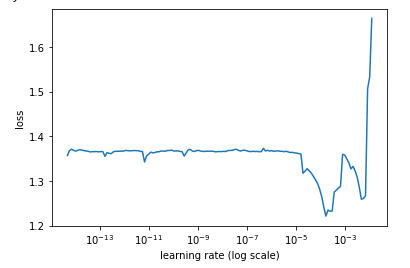
\includegraphics[width=0.7\textwidth]{./images/learning_rate_plot.png}
    \caption{Learning rate plot using Keras LRFinder}
    \label{fig:lr_plot}
\end{figure}

\subsubsection{Model A with Data Augmentation}
In order to see the influence that data augmentation has on our dataset, we decided to train two different models. Model A will implement data augmentation as exposed in Sec. \ref{ss:datapreparation} and Model B will implement the raw dataset.

Model A fit method can be seen in Lst. \ref{lst:fit-method:A}. Since we are using image augmentation and keras generator generates an unlimited number of images from our dataset we decided to show the algorithm only 100 images per epoch. Therefore, having 400 epochs would mean that the model process 40'000 images generated from a the training set containing 604 images. Certain authors \cite{Shorten2019, mikolajcyk2018} would argue that providing the model with such a large quantity of generated images would bias our results towards our own data distribution and the model would not be able to generalize further. However, since our dataset stems from a very limited subset of the Asian population we believe that by design the results of the model would already be biased towards the anatomic features of Asian eyes. Nevertheless, we implemented a cross validation method using 20\% of the original dataset whose results indicate that our training is not overfitting the data\footnote{See Sec. \ref{Results}}. Therefore, we do not believe that our model's ability to generalize the dataset is influenced by the number of images generated but the results are clearly biased towards a the Asian population and would be probably more successful for that kind of samples. The bias problem could only be solved by adding data from different populations so the model learns the characteristics of the human eye from all kinds of different humans. 

\begin{lstlisting}[caption={Model A training parameters, this is a code snippet from the  \emph{train\_model\_A} method in \emph{train.py}}, label={lst:fit-method:A}]
history = model.fit(train_generator,
                    steps_per_epoch = x_train.shape[0] // batch_size,
                    verbose=1, 
                    epochs=400, 
                    validation_data=(x_test, y_test_cat),
                    shuffle=True,
                    callbacks= [
                                ModelCheckpoint(monitor='val_loss',
                                filepath='weights/RMSProp_BCE_1e-4_best_weights.hdf5',
                                save_best_only=True,
                                save_weights_only=True),
                        ReduceLROnPlateau(monitor='val_loss',
                                          factor=0.1,
                                          patience=30,
                                          verbose=1,
                                          min_delta=1e-4),
                        TensorBoard(log_dir='./logs/syntethic_'+id ()),
                        CSVLogger('models/history'+id()+'.csv'),
                        EarlyStopping(monitor='val_loss',
                                      patience=70,
                                      verbose=1,
                                      min_delta=1e-4,
                                      baseline=0.2,
                                     )]
                   )
\end{lstlisting}

\subsubsection{Model B without Data Augmentation}

Model B was implemented over the raw dataset with the idea of cross validate the results and check the influence of image augmentation in our results. In this case, as seen in Lst. \ref{lst:fit-method-B} the input data comes directly from the numpy arrays created when splitting and converting the data to categorical in Lst.\ref{lst:data-split} and \ref{lst:data-categorical} 

\begin{lstlisting}[caption={Model B training parameters, this is a code snippet from the  \emph{train\_model\_B} method in \emph{train.py}},label={lst:fit-method-B}]
history = model.fit(x_train, y_train_cat,
                    batch_size=32,
                    verbose=1, 
                    epochs=100, 
                    validation_data=(X_test, y_test_cat), 
                    shuffle=True,
                    callbacks= [
                                ModelCheckpoint(monitor='val_loss',
                                filepath='weights/RMSProp_BCE_1e-4_best_weights.hdf5',
                                save_best_only=True,
                                save_weights_only=True),
                        ReduceLROnPlateau(monitor='loss',
                                          factor=0.1,
                                          patience=30,
                                          verbose=1,
                                          epsilon=1e-4),
                        TensorBoard(log_dir='./logs/syntethic_'+id),
                        CSVLogger('models/history'+id+'.csv'),
                        EarlyStopping(monitor='loss',
                                      patience=30,
                                      verbose=1,
                                      min_delta=1e-4,
                                      baseline=0.1,
                                      restore_best_weights=True)]
                   )

\end{lstlisting}

\subsection{Model Evaluation}
In order to evaluate the performance of our models we use different measures including Jaccard coefficient also called Intersection over Union (IoU). This measure is typically used to evaluate the similarity between two arbitrary shapes and is invariant to the scale of the problem considered because it encodes the shape properties of the objects being compared in the region property before computing a normalized measure that focuses on their surface\cite{IoU:2019}.

\begin{figure}[H]
   \[ J(A,B) = \frac{|A\cap B|}{|A\cup B|}\]
   \caption{Jaccards Coefficient Formula}
\end{figure}

The Jaccard's similarity coefficient between two datasets A and B is the result of dividing the number of common features between A and B, by the number the total number of features of both datasets \cite{Niwattanakul2013}.
In image classification tasks that involve classifying individual pixels, this is equivalent to say the number of pixels that overlap in the prediction and the ground truth is divided by the total number of pixels of the image. This measure allows us to compare the similarity between our model prediction and the ground truth by returning the percentage of correctly classified pixels. 
We have decided against accuracy as a performance measure in our project, since it doesn't offer an accurate measure of the performance for semantic segmentation tasks. Accuracy is measured by the number of correct predictions out of the total number of predictions. Suppose that we have 97\% accuracy, it means that 3\% of the pixels are not well classified, with a 500x768 image this gives us 11'250 misclassified pixels. This result does not offer any information about how the model performs at a class level. Furthermore, since in semantic segmentation is common to have classes whose weight in the final image is higher than others they will be overrepresented against minor classes in the final result. The reason is because there are significantly more pixels that will be correctly classified than those within a class with low weight. 
A confusion matrix allows to evaluate the model performance in a simple way to compare the predicted values with the ground-truth and can be represented like this \cite{ConfusionMatrix}:
    \begin{table}[H]
        \begin{tabular}{lll}
        \cline{2-3}
            \multicolumn{1}{l|}{}                                 & \multicolumn{1}{l|}{\textbf{Predicted Negative}} & \multicolumn{1}{l|}{\textbf{Predicted positive}} \\ \hline
            \multicolumn{1}{|l|}{\textbf{Ground-truth Negative}} & \multicolumn{1}{l|}{True negative (TN)}          & \multicolumn{1}{l|}{False Positive (FP)}         \\ \hline
            \multicolumn{1}{|l|}{\textbf{Ground-truth Positive}}  & \multicolumn{1}{l|}{False Negative (FN)}         & \multicolumn{1}{l|}{True Positive (TP)}          \\ \hline
        \end{tabular}
        \caption{Confusion Matrix}
    \end{table}

Using the confusion matrix we can then compute two metrics that we use for model evaluation: sensitivity and specificity. 
The sensitivity can be described as the proportion classified pixels among the true positive, it shows the rate of relevant pixels that were correctly classified. 

The specificity measures the ability to correctly reject the pixels that do not belong in a class. In other words the number of true negatives divided by the sum of the true negatives and false positives. Sensitivity measures  the proportion of actual positive cases that were correctly predicted, while specificity is used to determine the proportion of actual negative cases that were correctly predicted, giving a sense of the ability of our model to reject pixels that do not belong to a certain class. 


\section{Results}

\begin{figure} \label{fig:results_modelA}
   \centering
   \begin{subfigure}{1\textwidth}
    \centering
    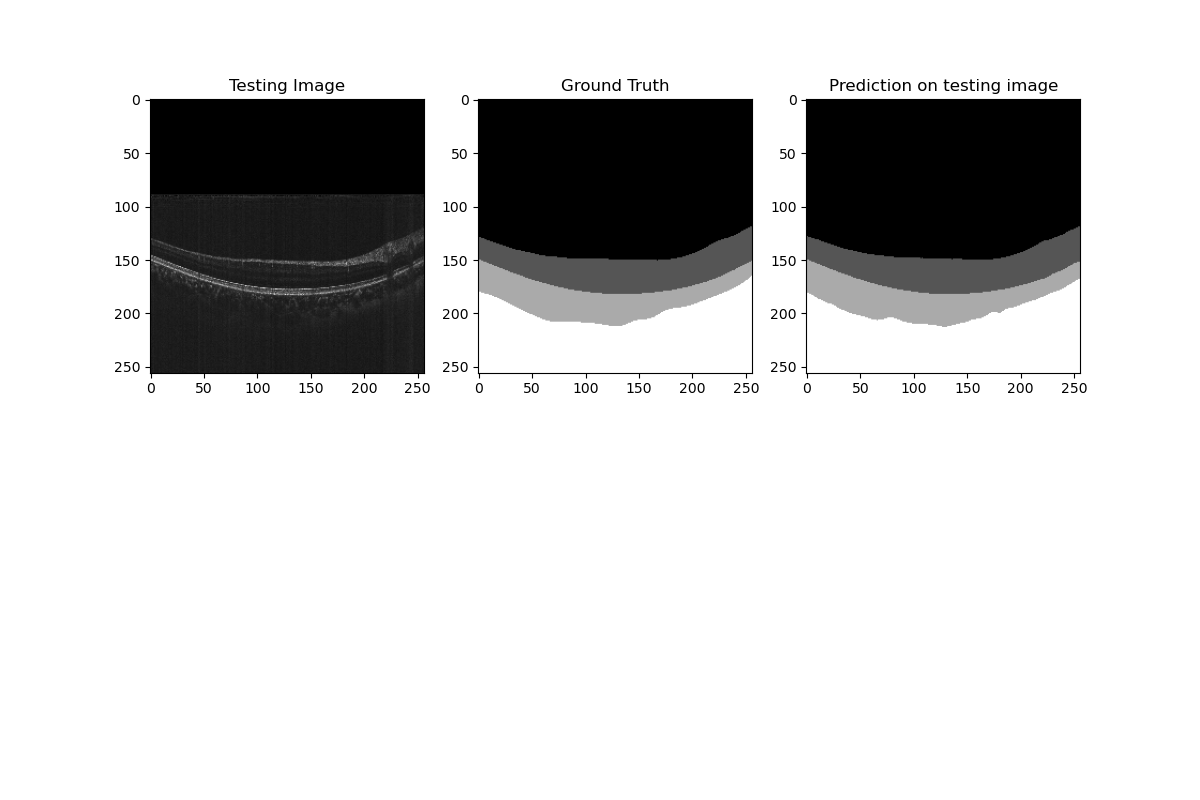
\includegraphics[trim= 100 250 80 0, clip, width=0.85\textwidth]{./images/results/A_syntethic_groundtruth_predictions29052021-112413_0.png}
    \caption{}
    \label{fig:results:A:a}
   \end{subfigure}
   \begin{subfigure}{1\textwidth}
    \centering
    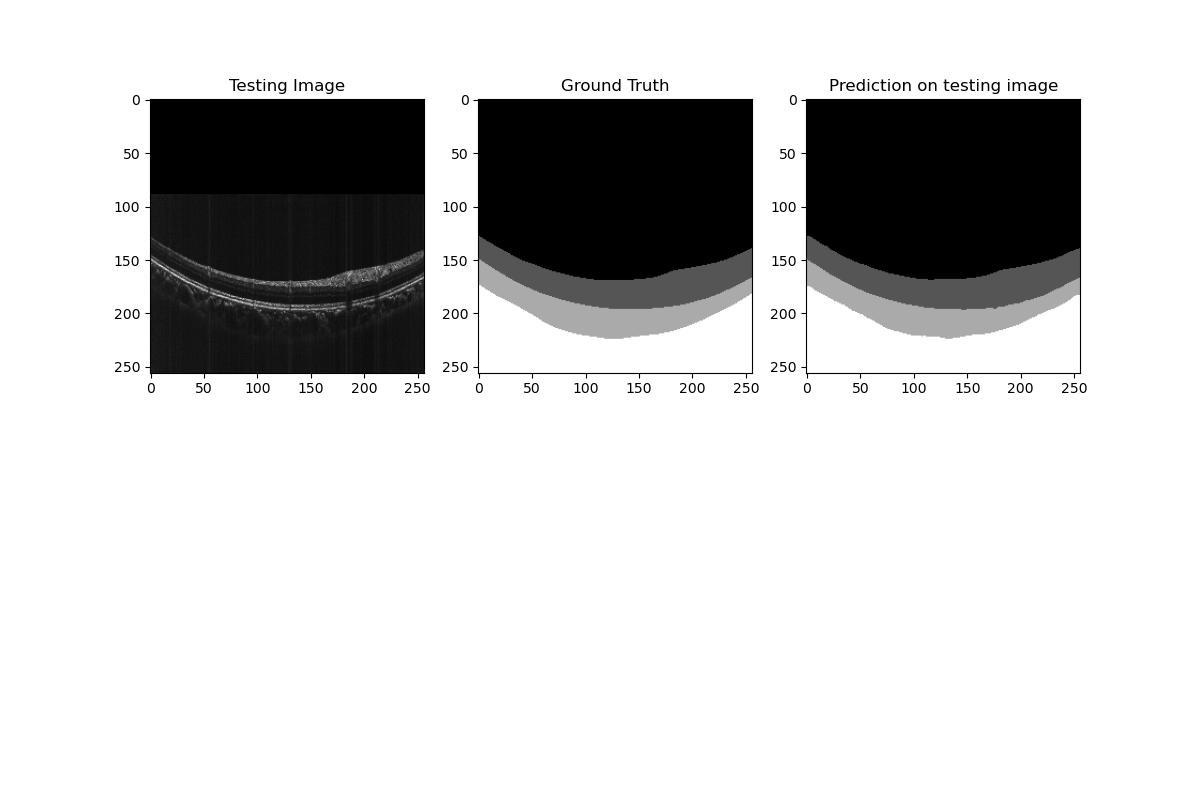
\includegraphics[trim= 100 250 80 0, clip, width=0.85\textwidth]{./images/results/A_syntethic_groundtruth_predictions29052021-112417_4.png}
    \caption{}
    \label{fig:results:A:b}
   \end{subfigure}
    \begin{subfigure}{1\textwidth}
    \centering
    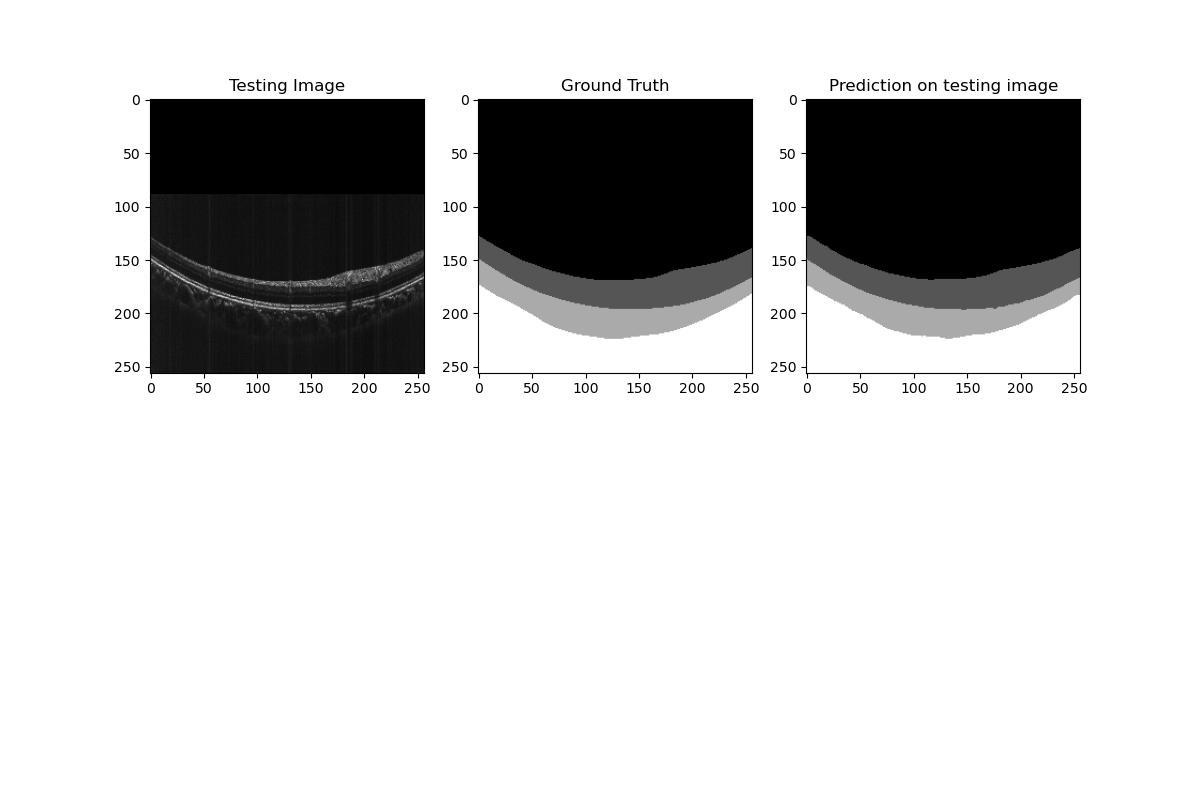
\includegraphics[trim= 100 250 80 0, clip, width=0.85\textwidth]{./images/results/A_syntethic_groundtruth_predictions29052021-112416.png}
    \caption{}
    \label{fig:results:A:c}
   \end{subfigure}
   \caption{Results of the CNN's prediction on the validation set of Model A}
  \label{Results}
\end{figure}

\begin{figure} 
   \centering
   \begin{subfigure}{1\textwidth}
    \centering
    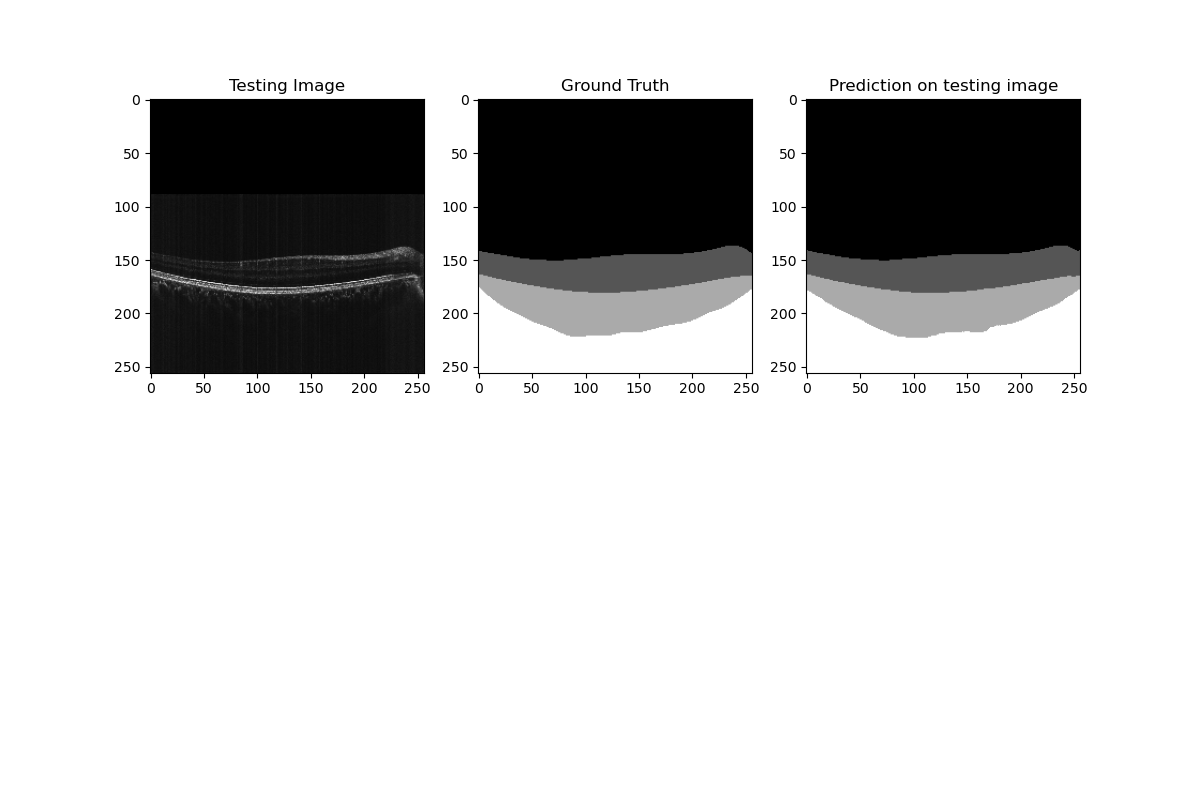
\includegraphics[trim= 100 250 80 0, clip, width=0.85\textwidth]{./images/results/B_syntethic_groundtruth_predictions29052021-081035_0.png}
    \caption{}
    \label{fig:results:B:a}
   \end{subfigure}
   \begin{subfigure}{1\textwidth}
    \centering
    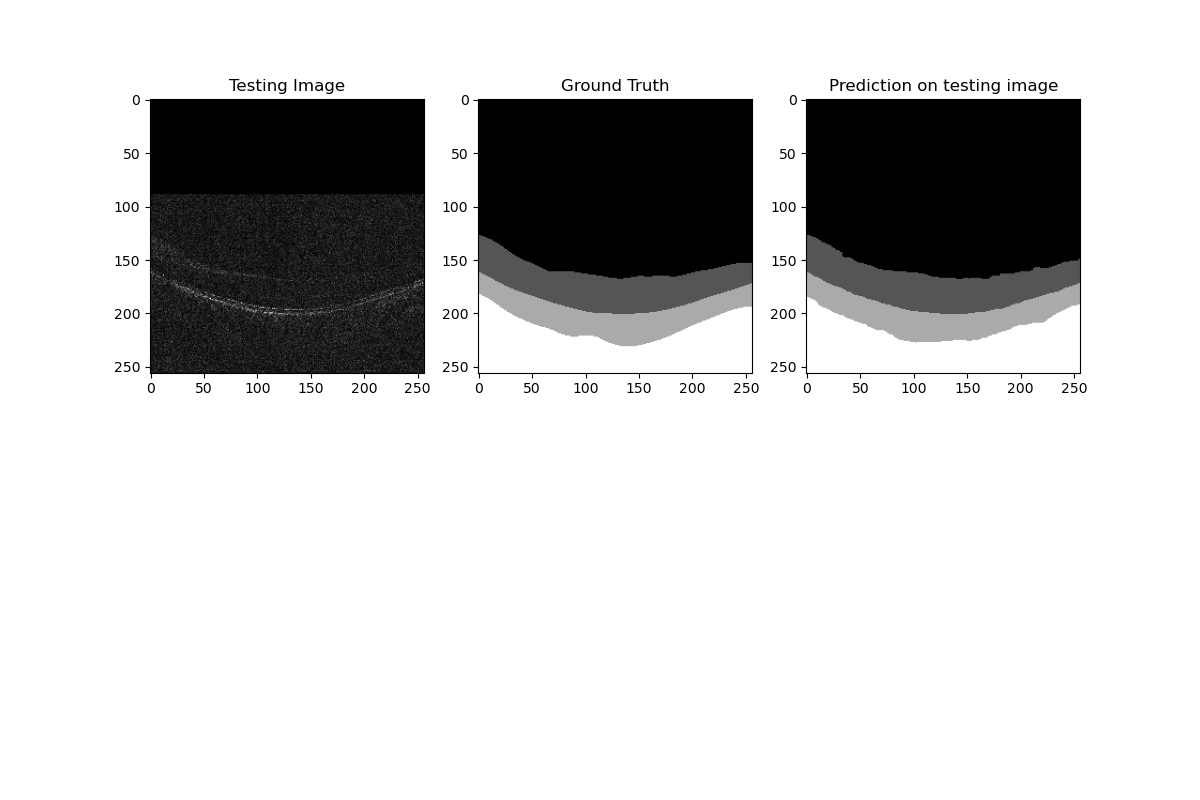
\includegraphics[trim= 100 250 80 0, clip, width=0.85\textwidth]{./images/results/B_syntethic_groundtruth_predictions29052021-081035_4.png}
    \caption{}
    \label{fig:results:B:b}
   \end{subfigure}
    \begin{subfigure}{1\textwidth}
    \centering
    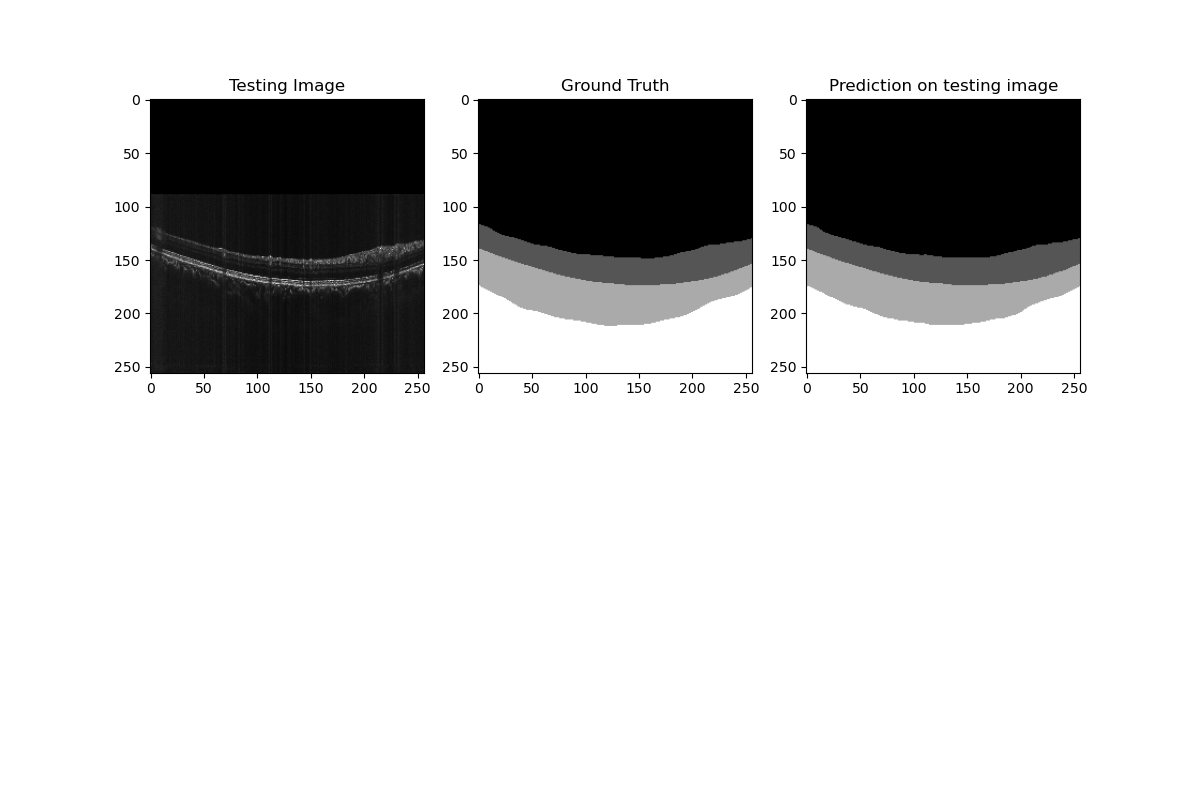
\includegraphics[trim= 100 250 80 0, clip, width=0.85\textwidth]{./images/results/B_syntethic_groundtruth_predictions29052021-081035.png}
    \caption{}
    \label{fig:results:B:c}
   \end{subfigure}
   \caption{Results of the CNN's prediction on the validation set of Model B}
  \label{fig:results_modelB}
\end{figure}

After training and cross validation, Model A had a mean Jaccard's coefficient of 96.78\% on the validation set. On a class level, the results were slightly better on the vitreous with 99.55\%, 96.97\% for retina, 94.16\% for choroid and 96.41\% for sclera.
The model had a mean of 97.80\% sensitivity referring to the overall ability to classify accurately relevant pixels. On the other end, the mean specificity was 99.52\% which means that the model presents a high performance at rejecting pixels whenever they do not belong to a certain class. 

Model B presented a mean Jaccard's coefficient of 98.01\%. On a class level the results were: 99.82\% for vitreous, 98.62\% for retina, 96.03\% for choroid and 97.59\% for sclera. Its sensibility was 96.72\% and mean specificity 99.65\%.

According to a similar research article called \emph{Validation of automated artificial intelligence segmentation of optical coherence tomography images}  published by Peter Maloca et al., their CNN predictions's mean Jaccard's coefficient for vitreous was 99.29\%, 96.90\% for retina, 88.17\% for choroid and 97.68\% for sclera, concluding that the CNN's compartmentalization of OCT scans was comparable to that of human graders. \cite{Maloca2019} 


\begin{figure}[H]
\centering
\begin{subfigure}{1\textwidth}
  \centering
  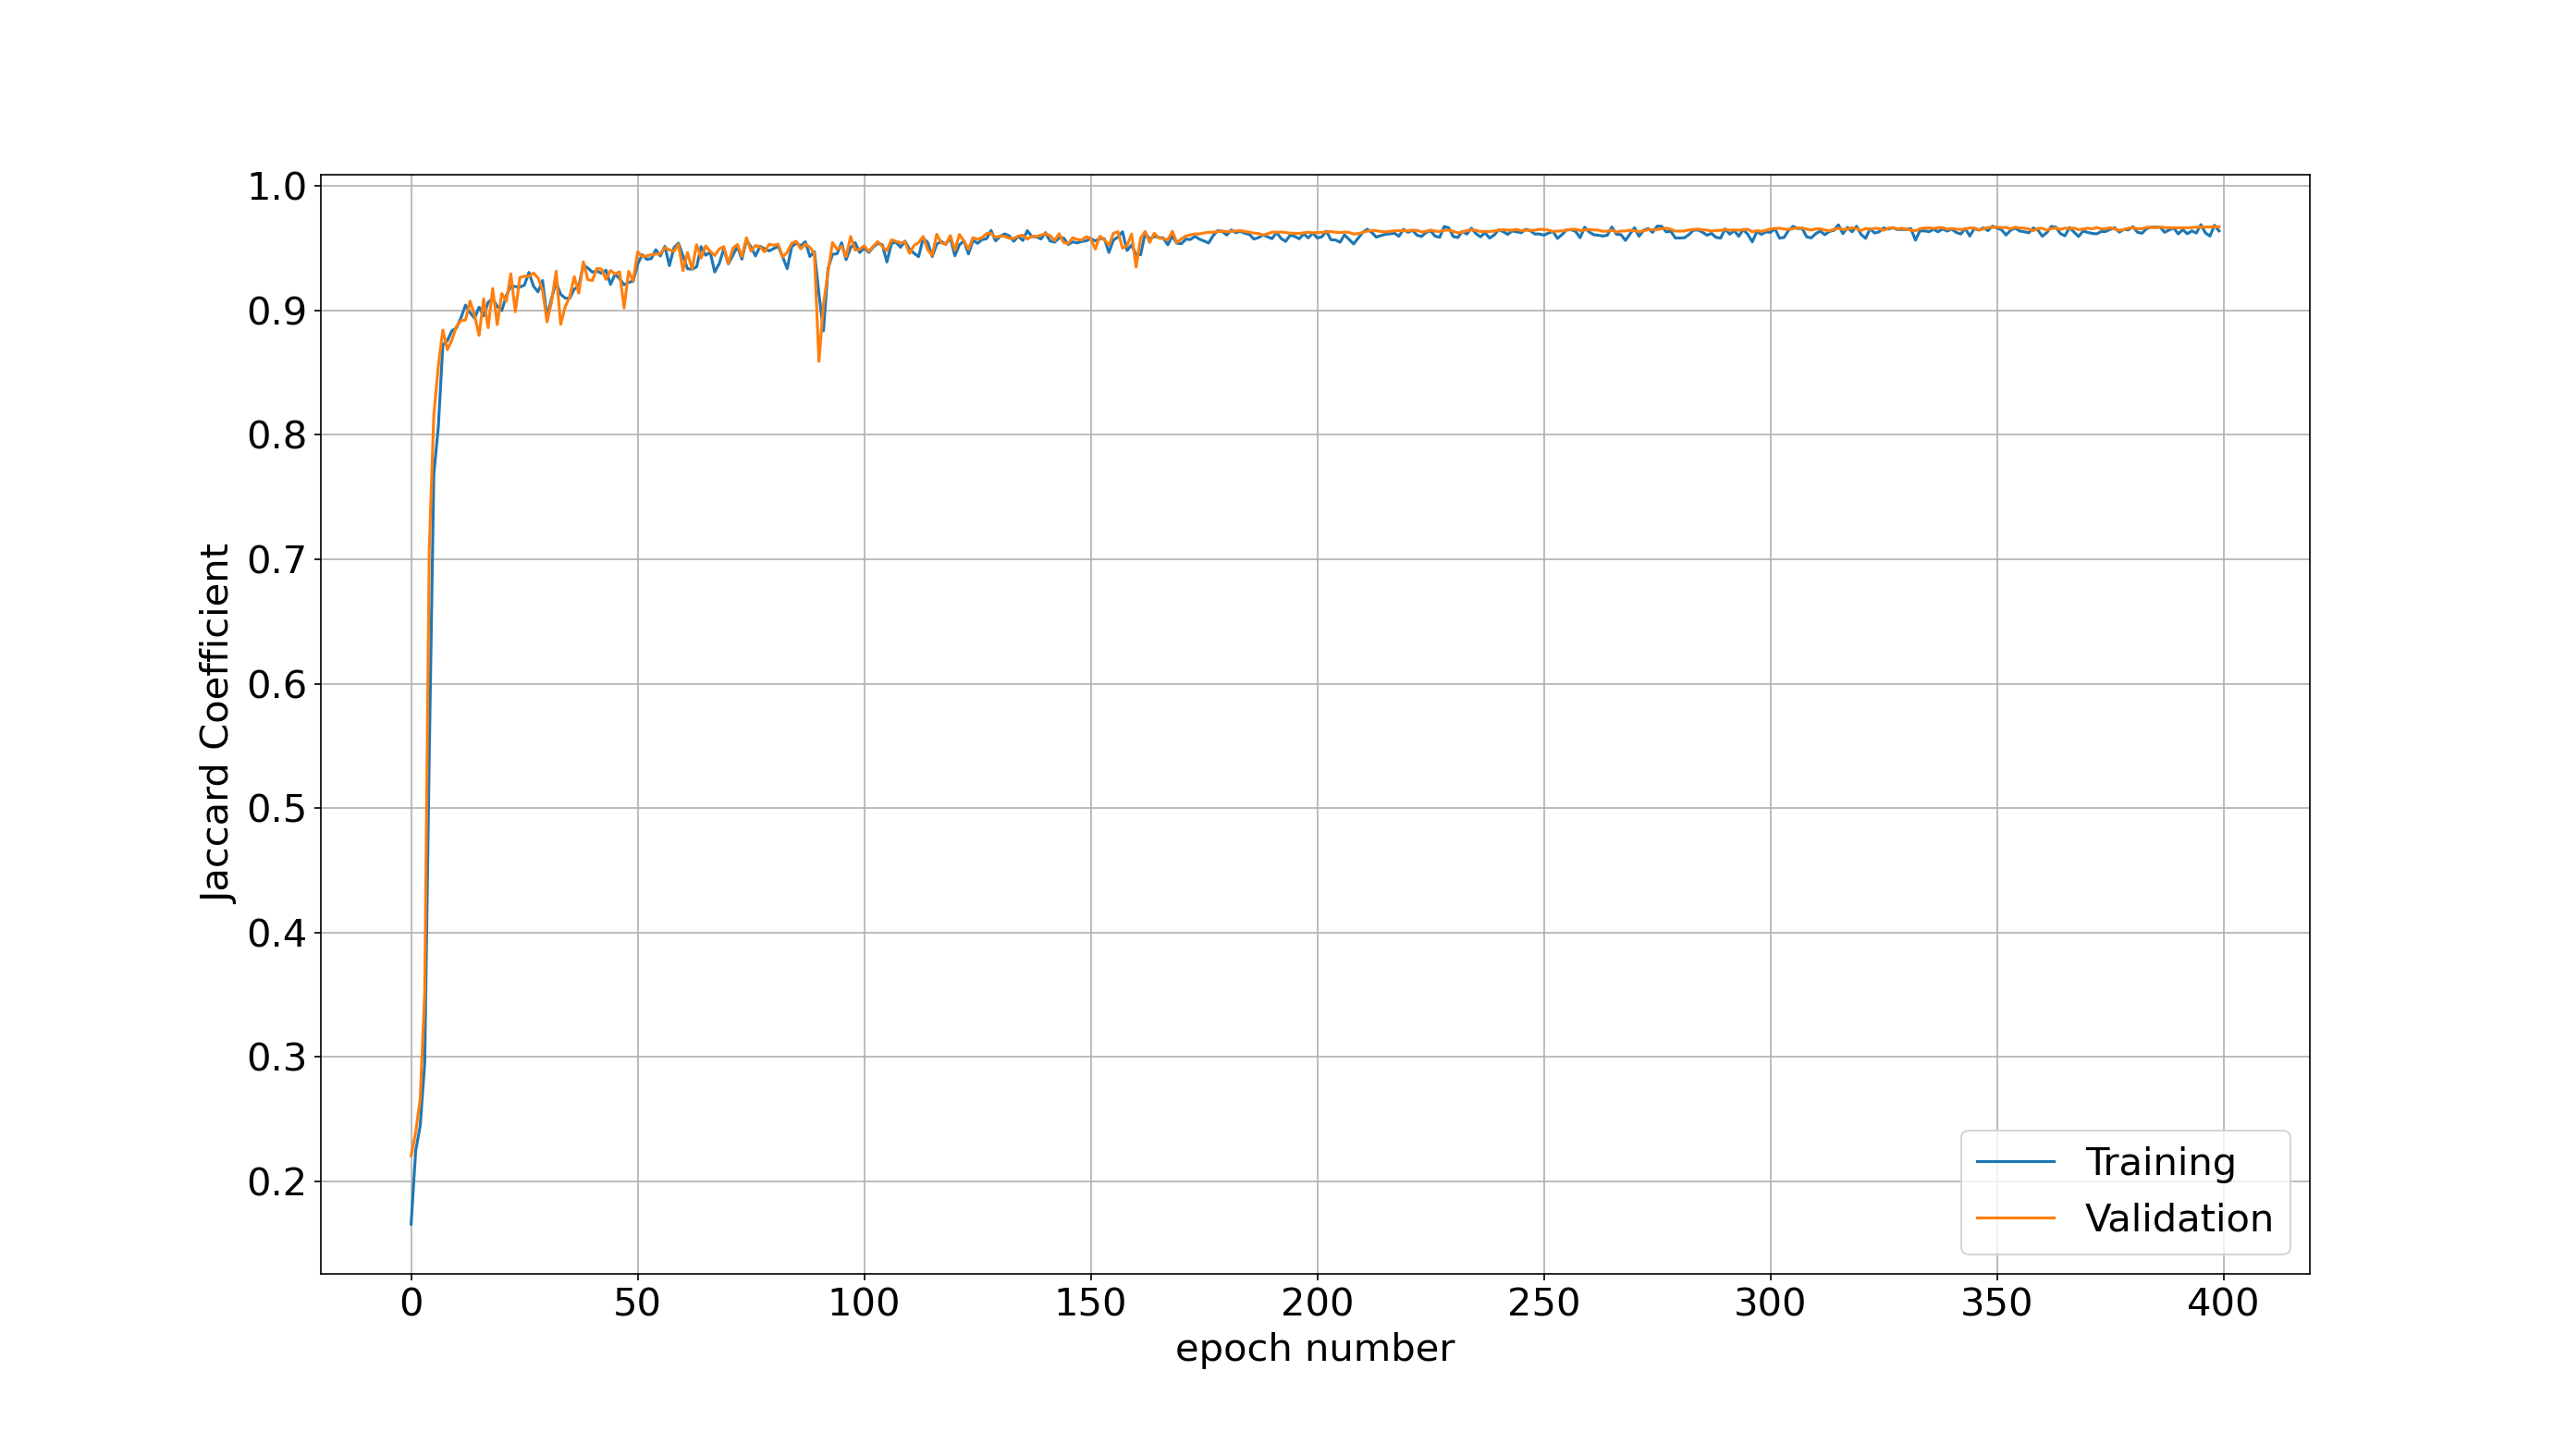
\includegraphics[width=\linewidth]{./results/model_a_jaccard.png}
  \caption{Model A}
  \label{fig:model_a_jaccard}
\end{subfigure}
\begin{subfigure}{1\textwidth}
  \centering
  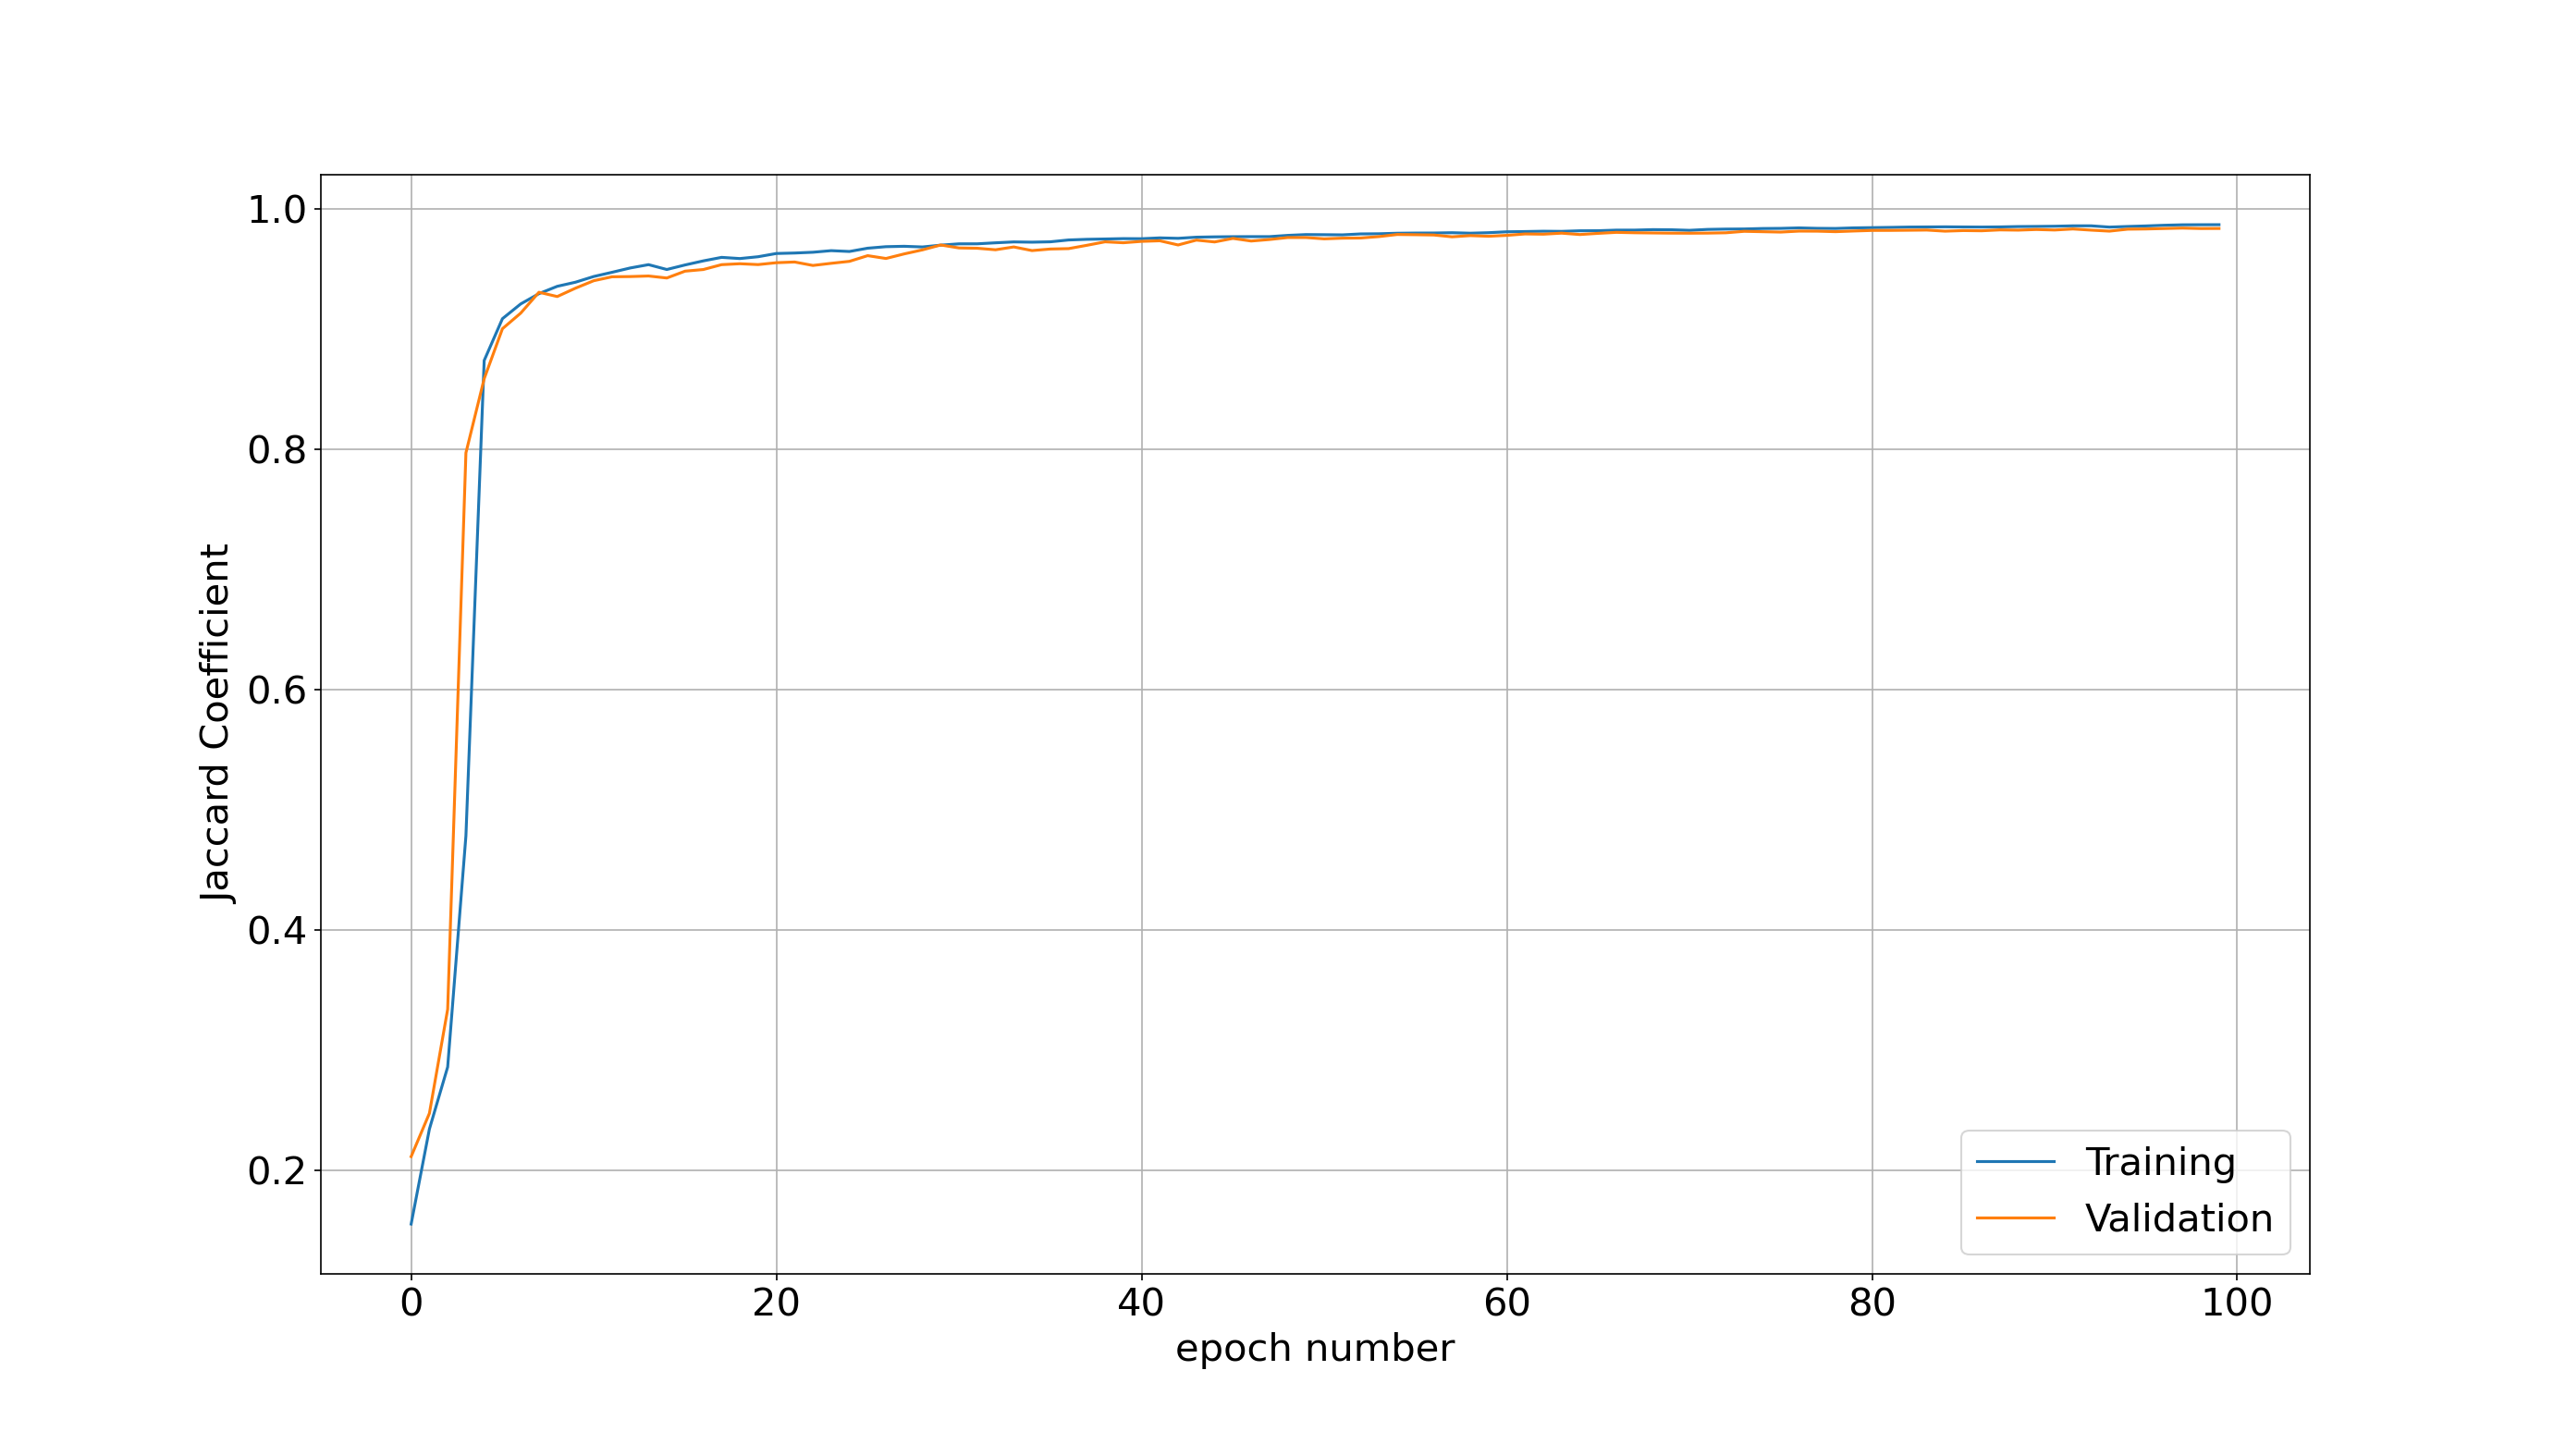
\includegraphics[width=\linewidth]{./results/model_b_jaccard.png}
  \caption{Model B}
  \label{fig:modelb_jaccard}
\end{subfigure}
\caption{Jaccard's Coefficient Results}
\label{fig:jaccard_results}
\end{figure}

\begin{figure}[H]
\centering
\begin{subfigure}{1\textwidth}
  \centering
  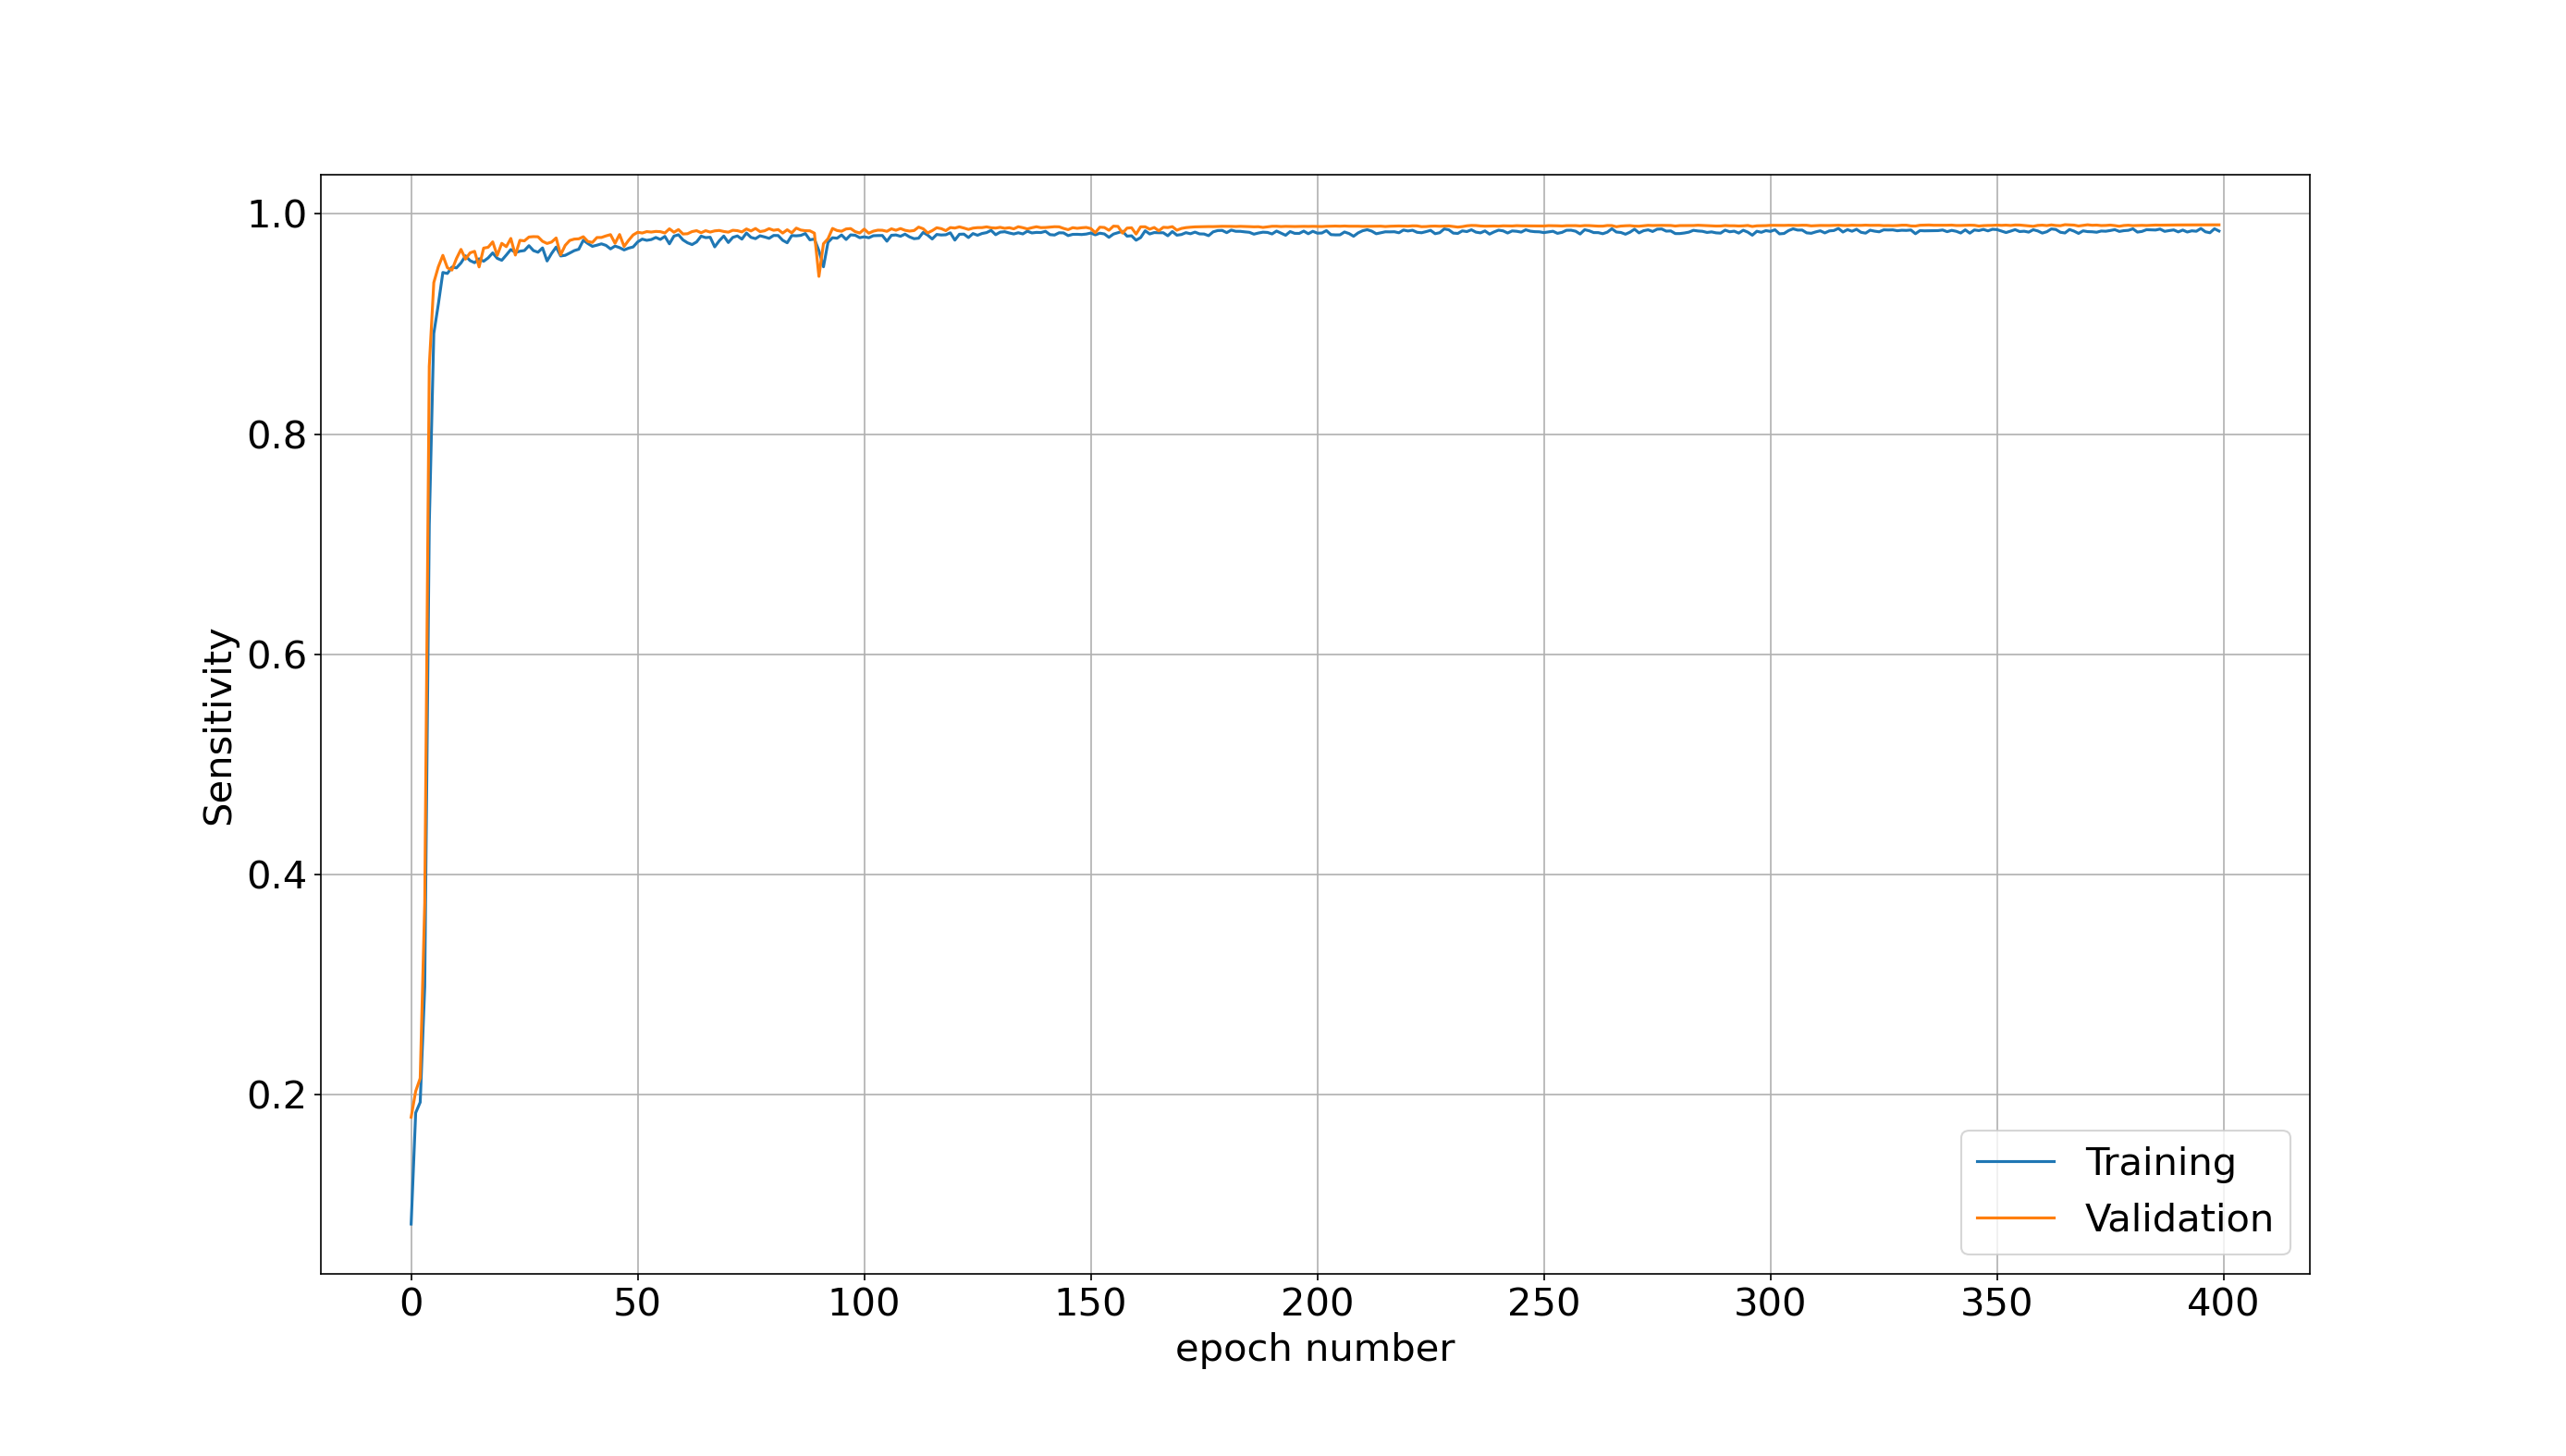
\includegraphics[width=\linewidth]{./results/model_a_sensitivity.png}
  \caption{Model A}
  \label{fig:model_a_sensitivity}
\end{subfigure}
\begin{subfigure}{1\textwidth}
  \centering
  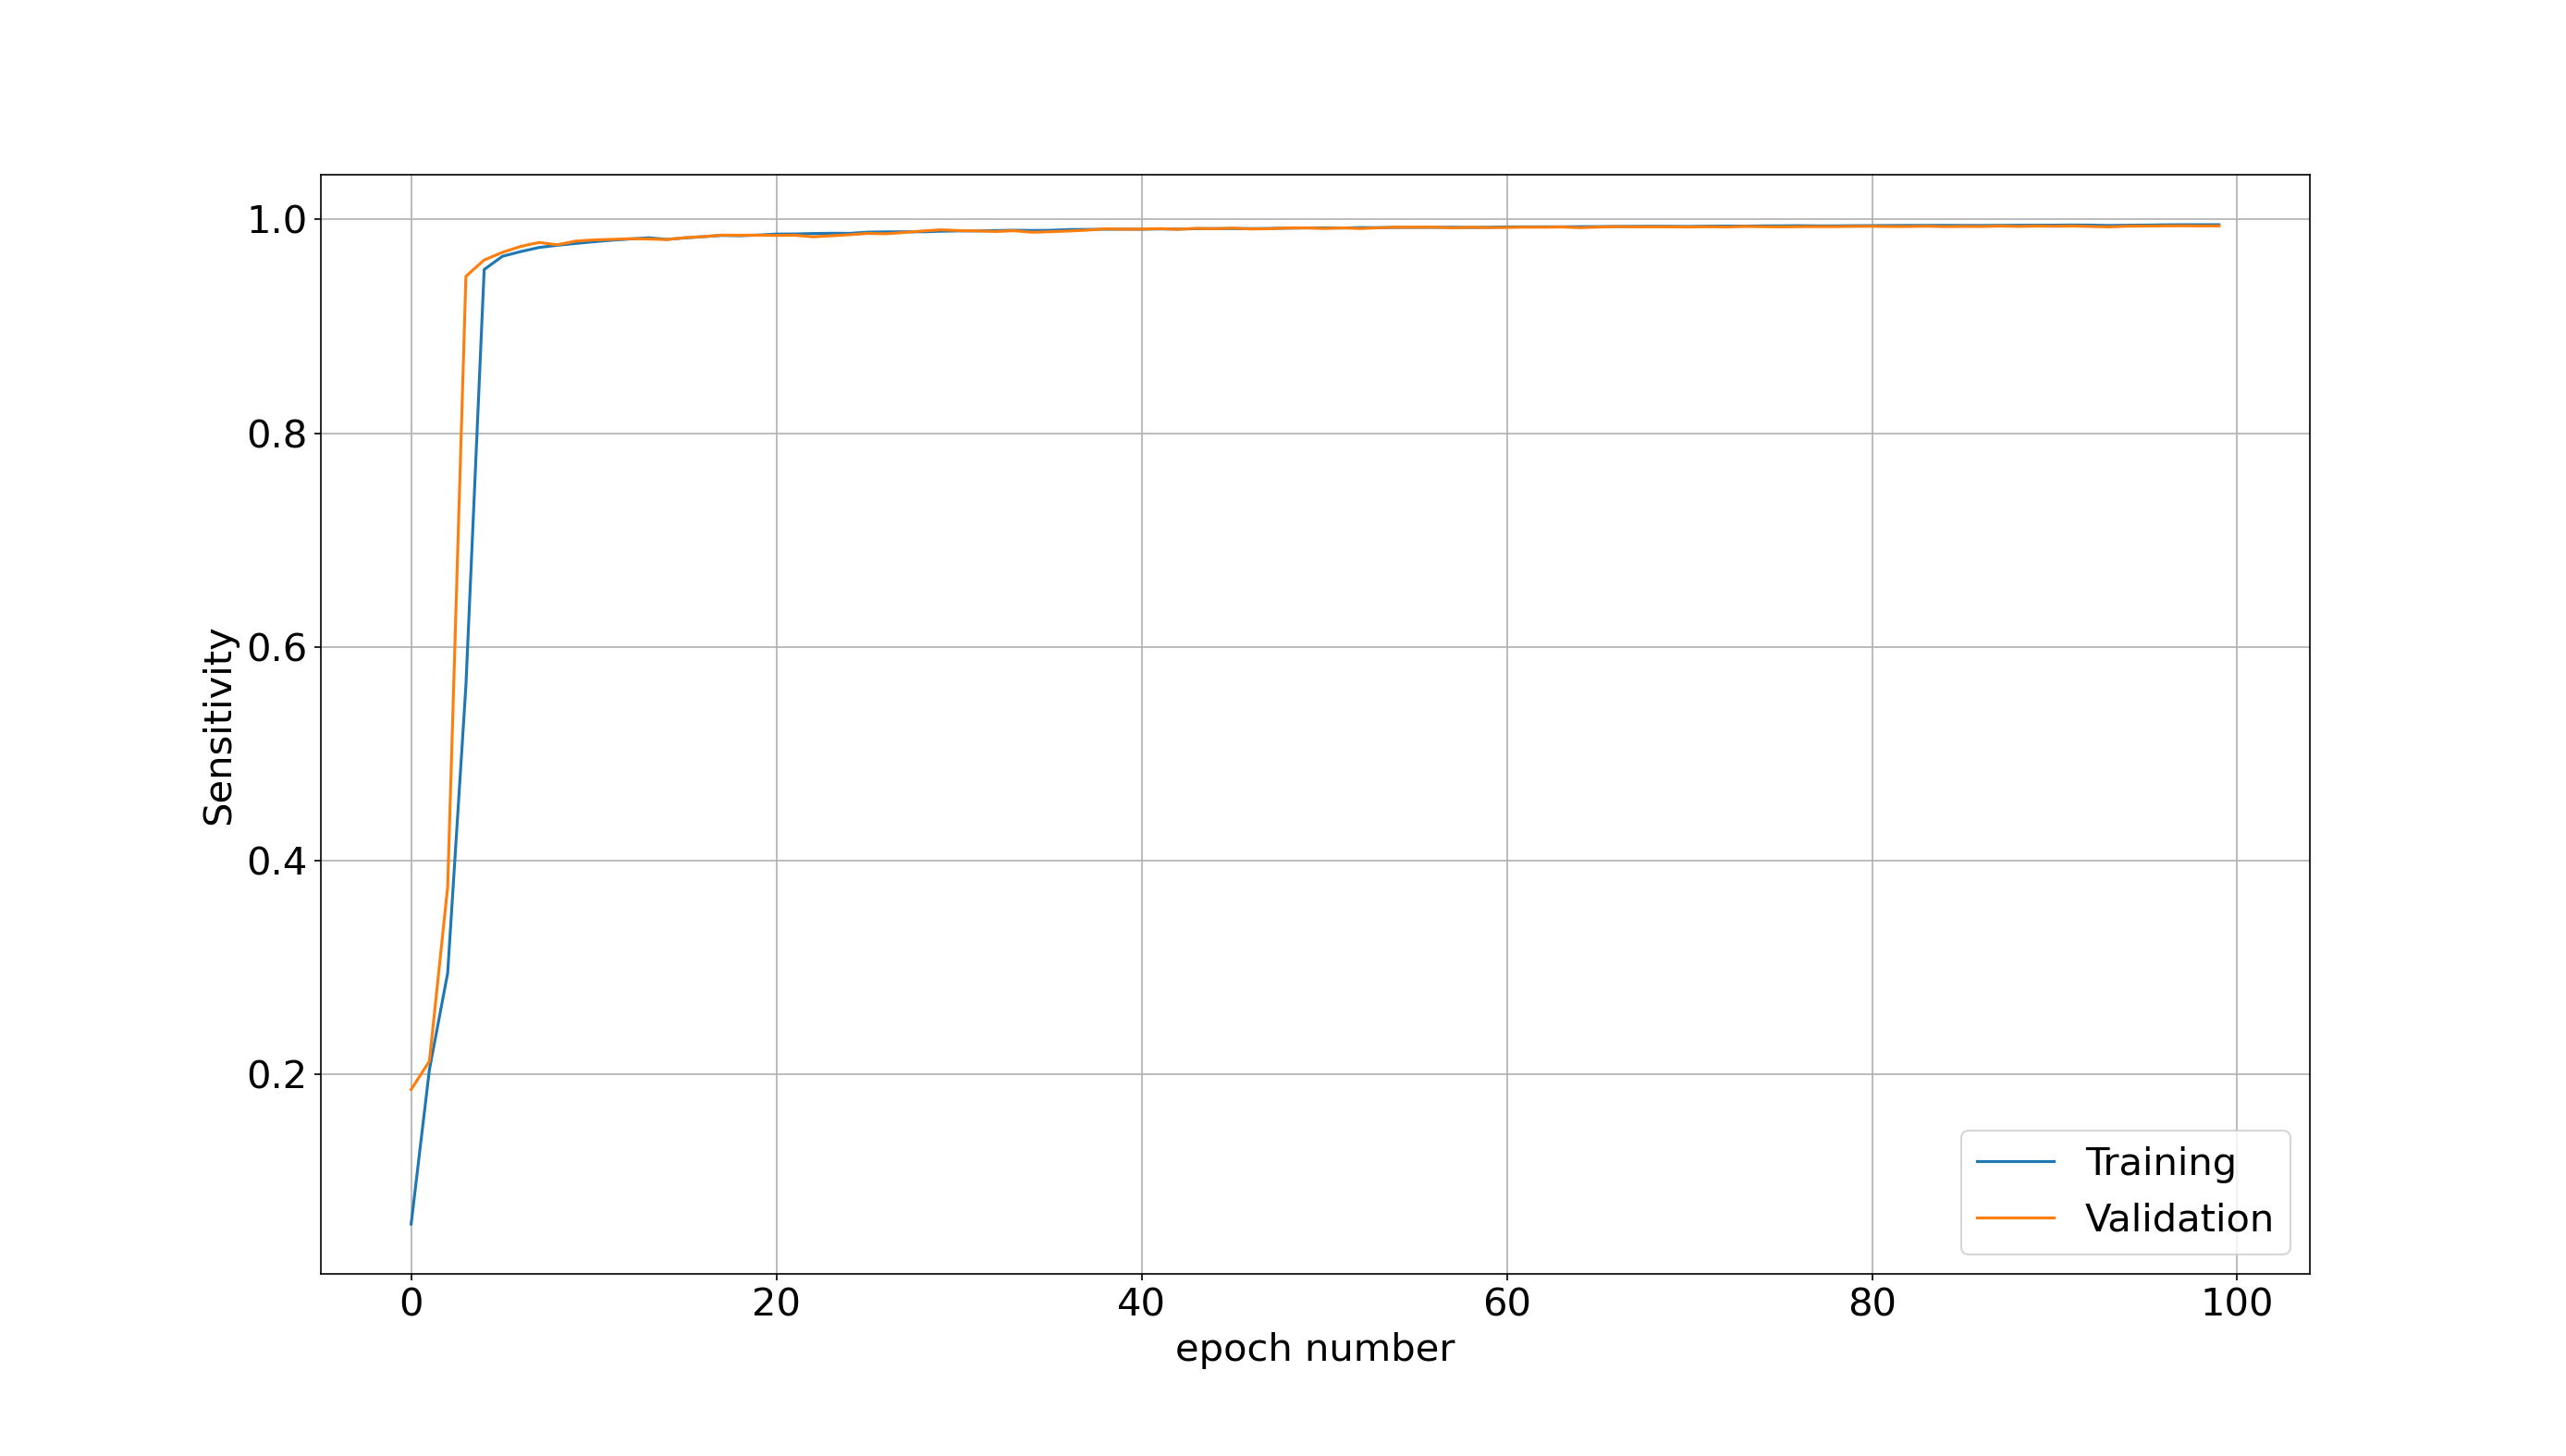
\includegraphics[width=\linewidth]{./results/model_b_sensitivity.png}
  \caption{Model B}
  \label{fig:modelb_sensitivity}
\end{subfigure}
\caption{Sensitivity Results}
\label{fig:sensitivity_results}
\end{figure}

\begin{figure}[H]
\centering
\begin{subfigure}{1\textwidth}
  \centering
  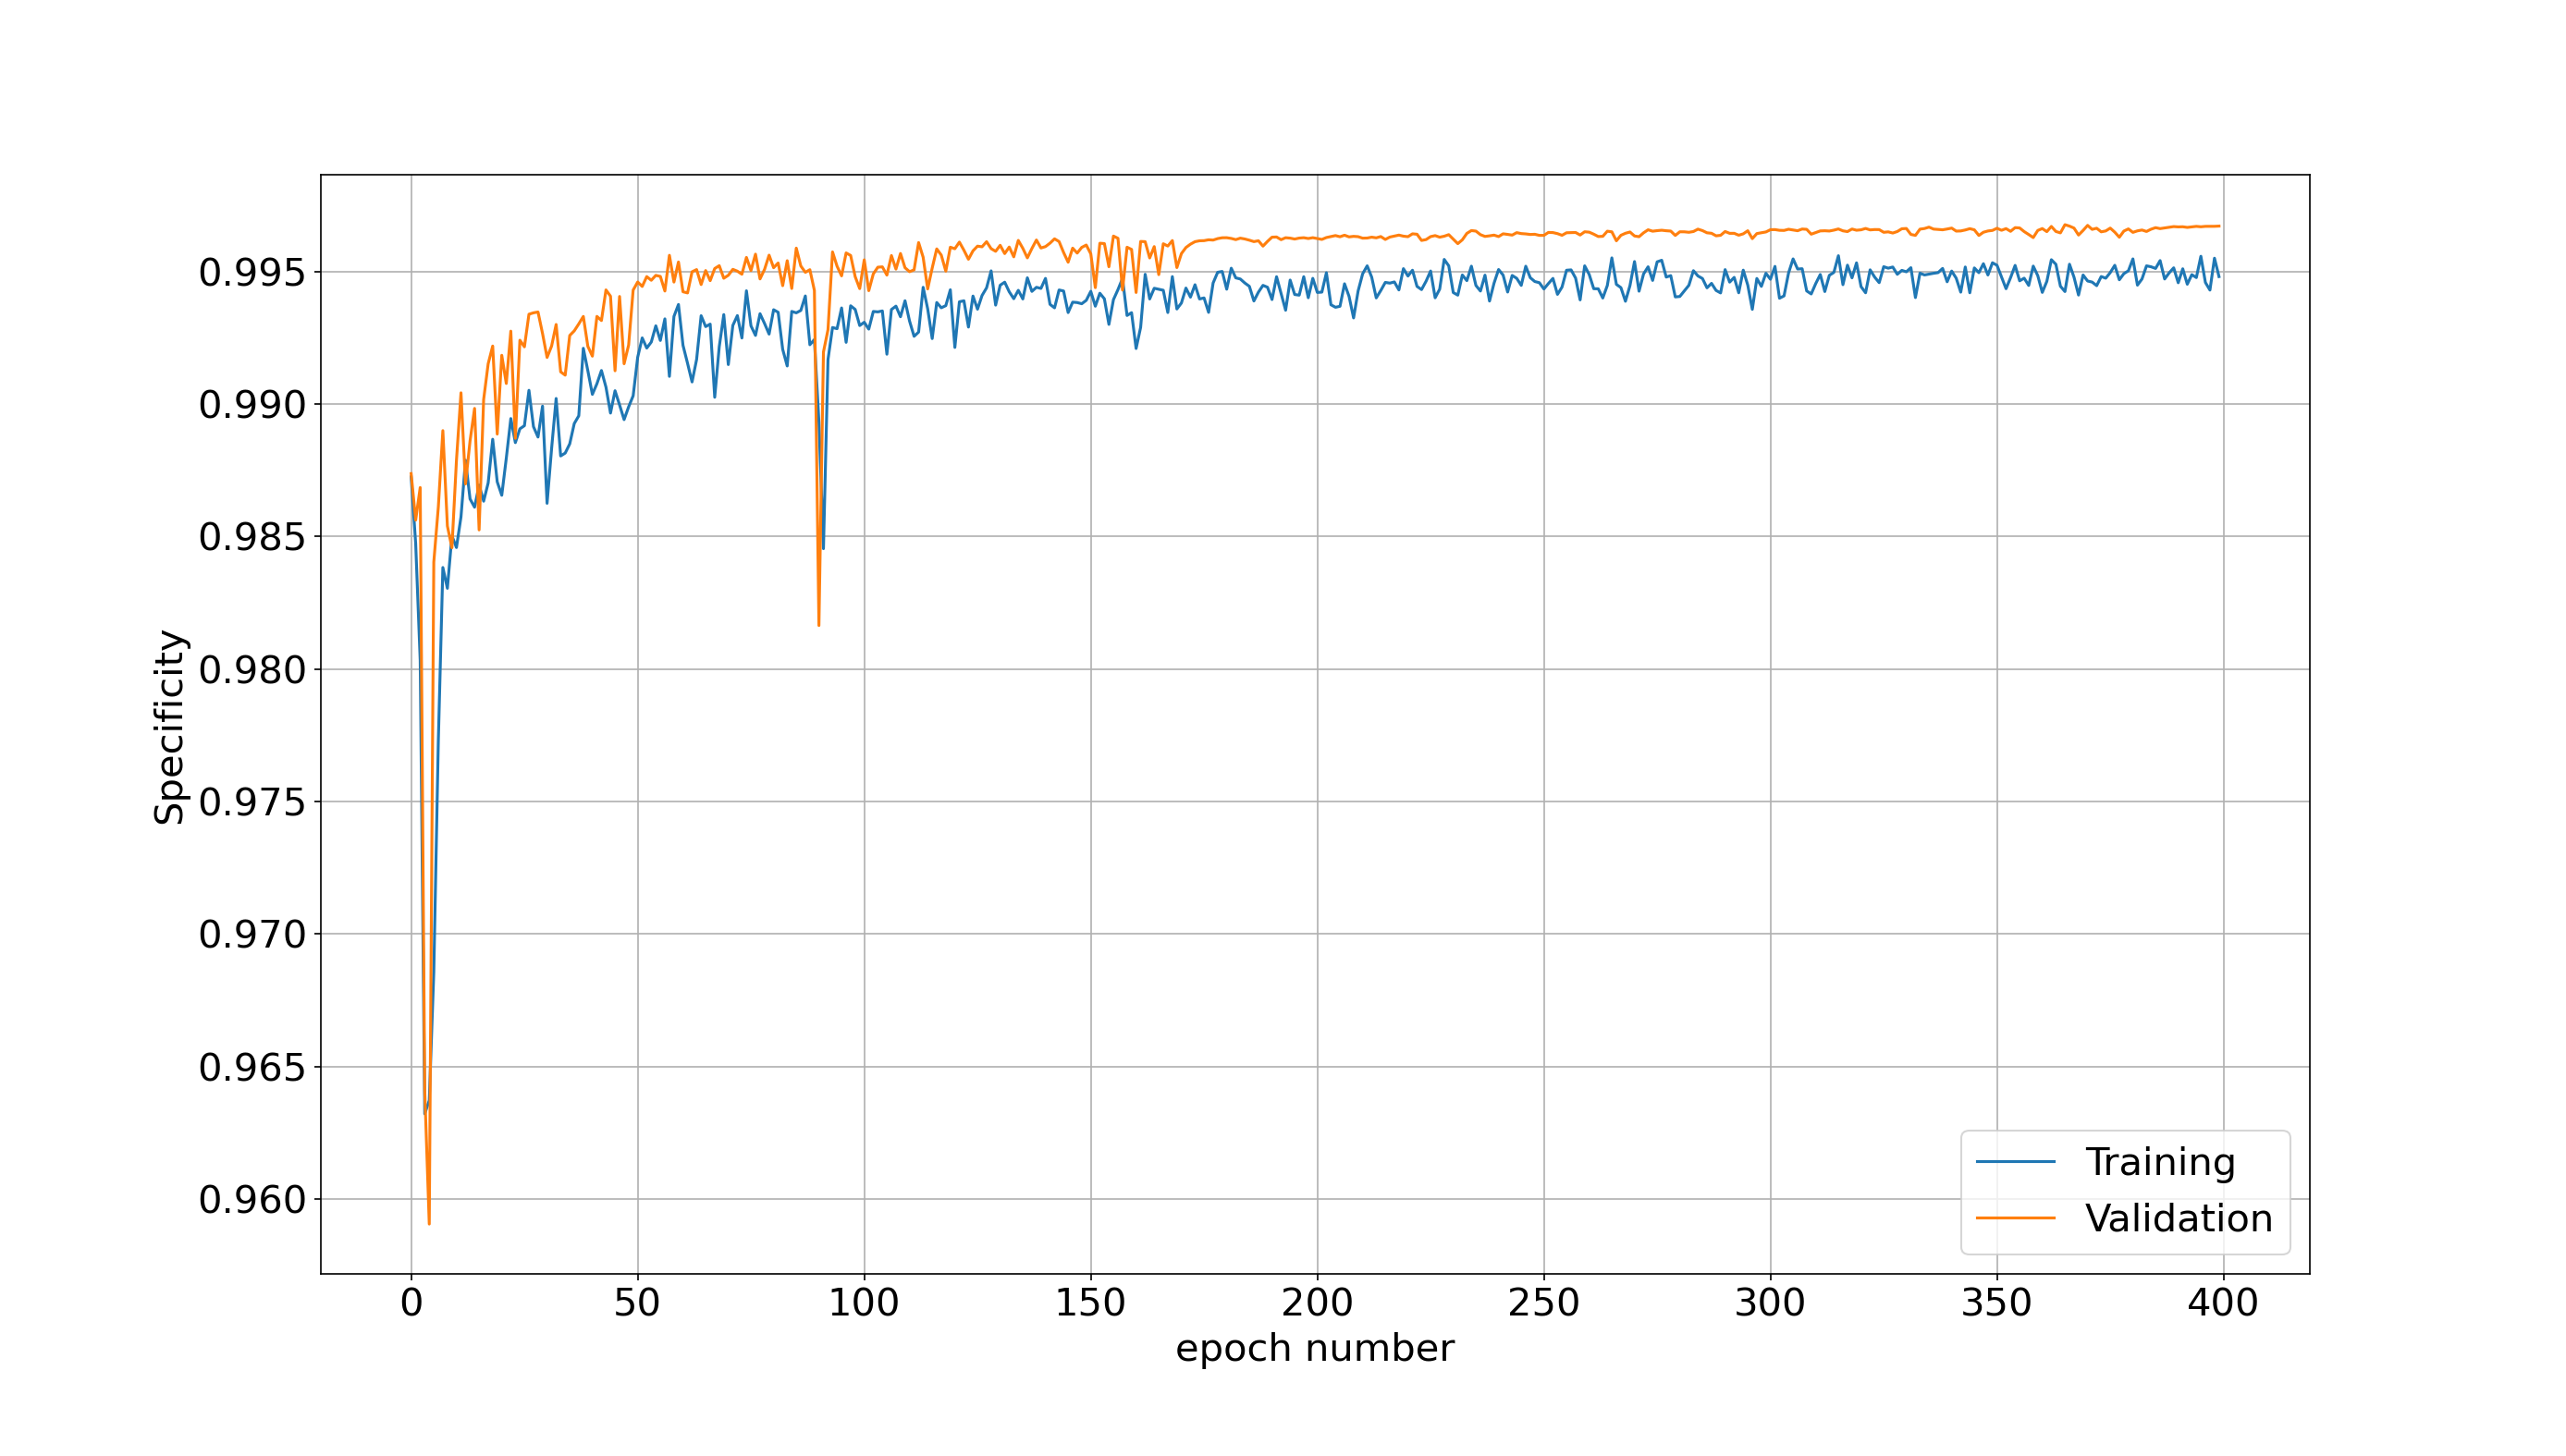
\includegraphics[width=\linewidth]{./results/model_a_specificity.png}
  \caption{Model A}
  \label{fig:model_a_specificity}
\end{subfigure}
\begin{subfigure}{1\textwidth}
  \centering
  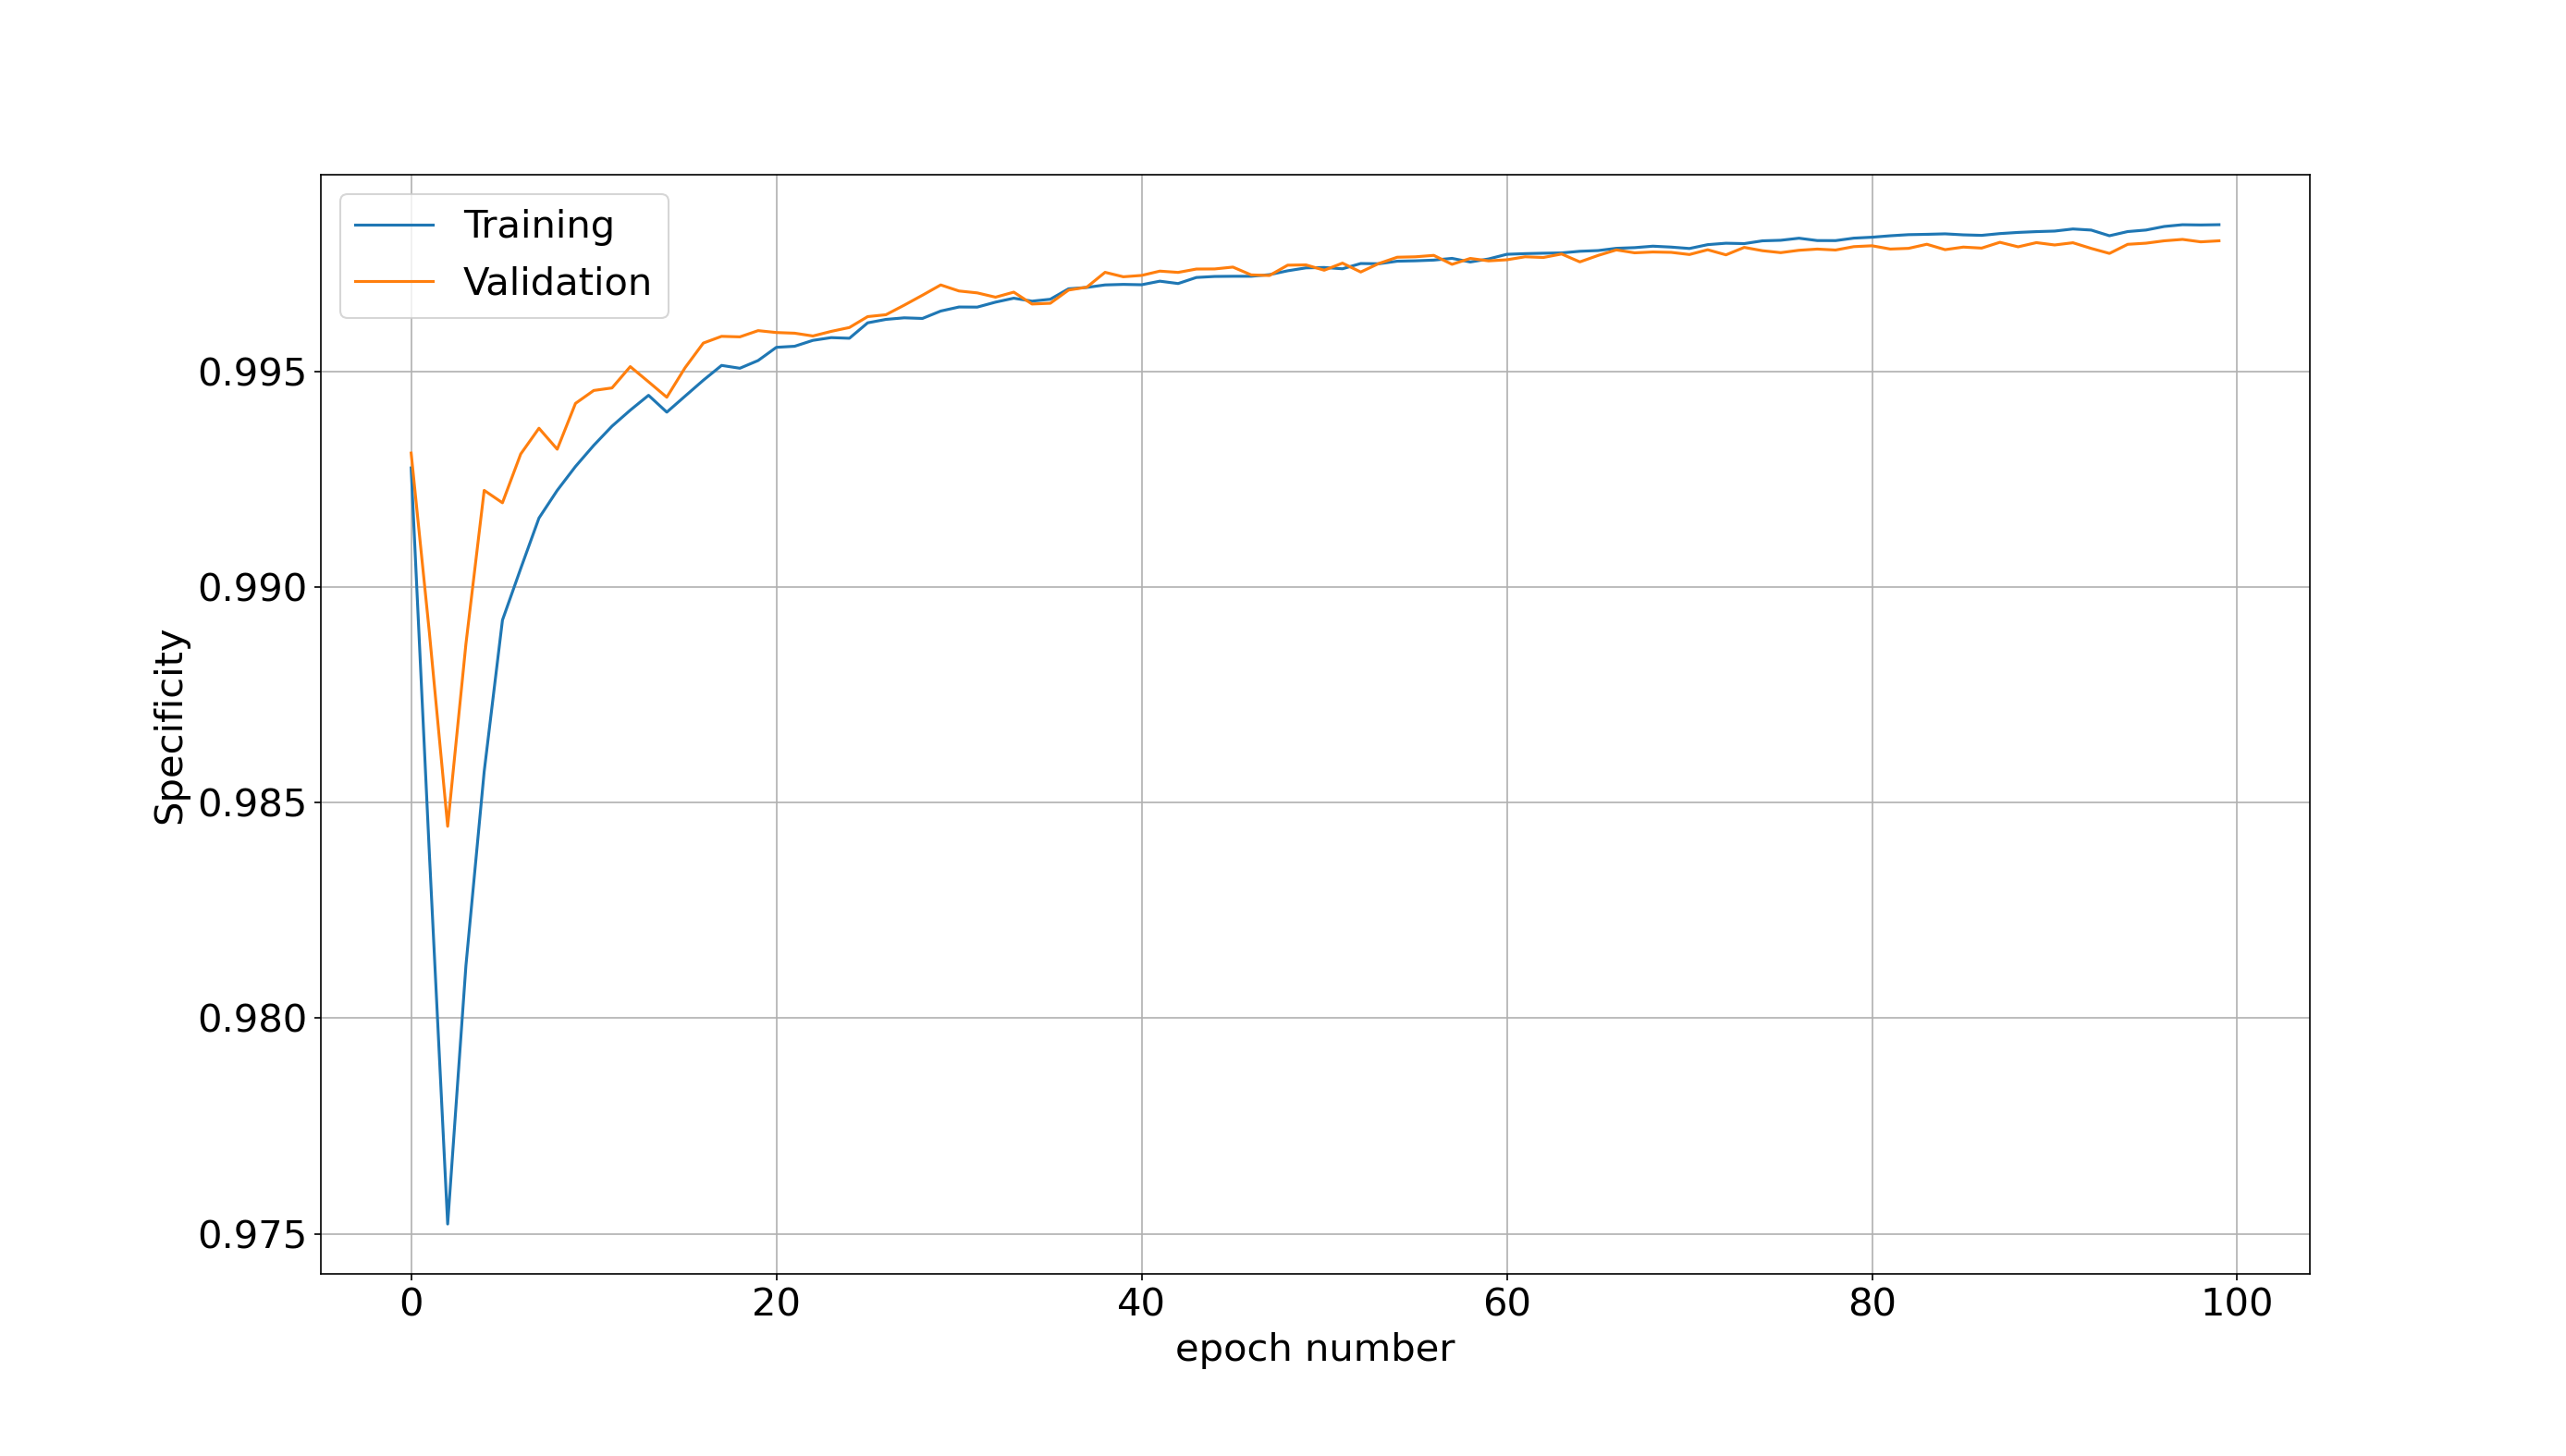
\includegraphics[width=\linewidth]{./results/model_b_specificity.png}
  \caption{Model B}
  \label{fig:modelb_specificity}
\end{subfigure}
\caption{Specificity Results}
\label{fig:specificity_results}
\end{figure}


In order to quantify the error between our models' output and the ground truth, the loss function needs to be minimized as stated in Sec. \ref{ss:model_training}. After 400 epochs Model A had a training loss of 0.046, validation loss was 0.038. For Model B the training lasted 100 epochs and the training loss was 0.016 and validation loss 0.027 as can be seen in Fig. \ref{fig:modelloss}. The fact that the trend in these two metrics remained similar between the training and validation stage and also tending to 0 indicates that our model is neither overfitting nor underfitting the data \cite{DIDLBook}. 

\begin{figure}[H]
   \centering
   \begin{subfigure}{1\textwidth}
    \centering
    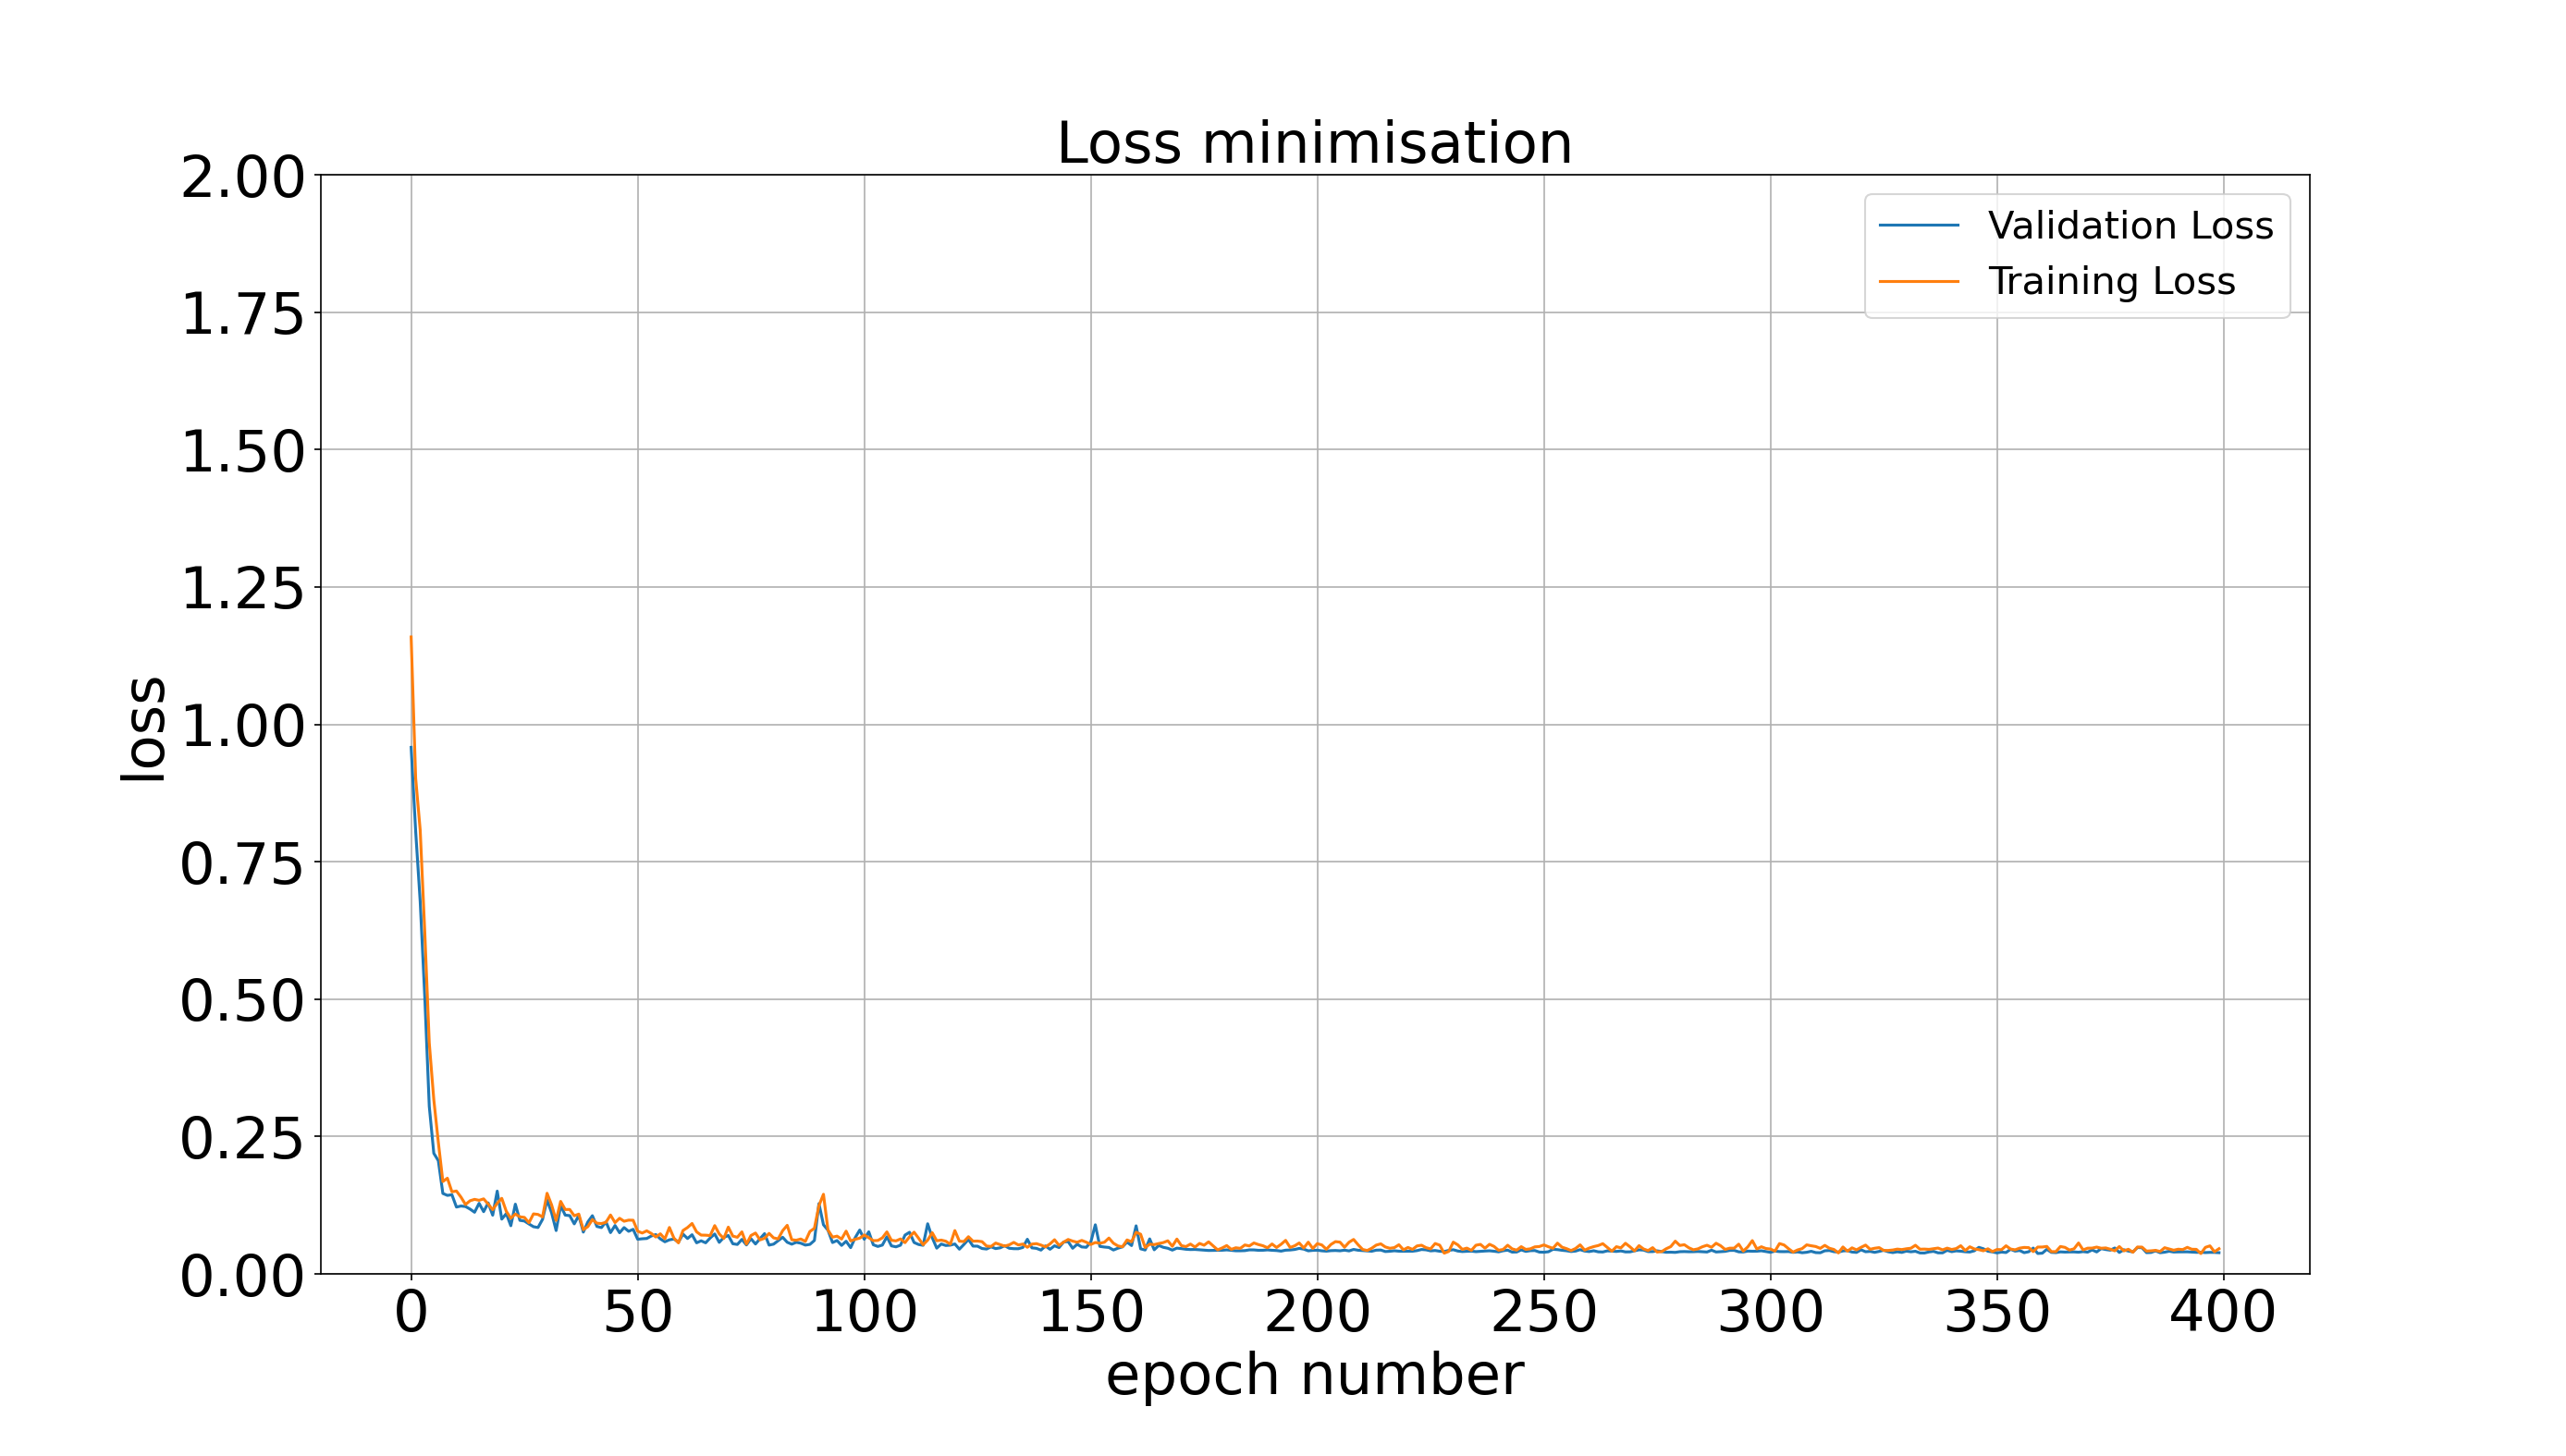
\includegraphics[ width=0.85\textwidth]{././images/results/modelA_loss_plot.png}
    \caption{Model A}
    \label{fig:loss_a}
   \end{subfigure}
   \begin{subfigure}{1\textwidth}
    \centering
    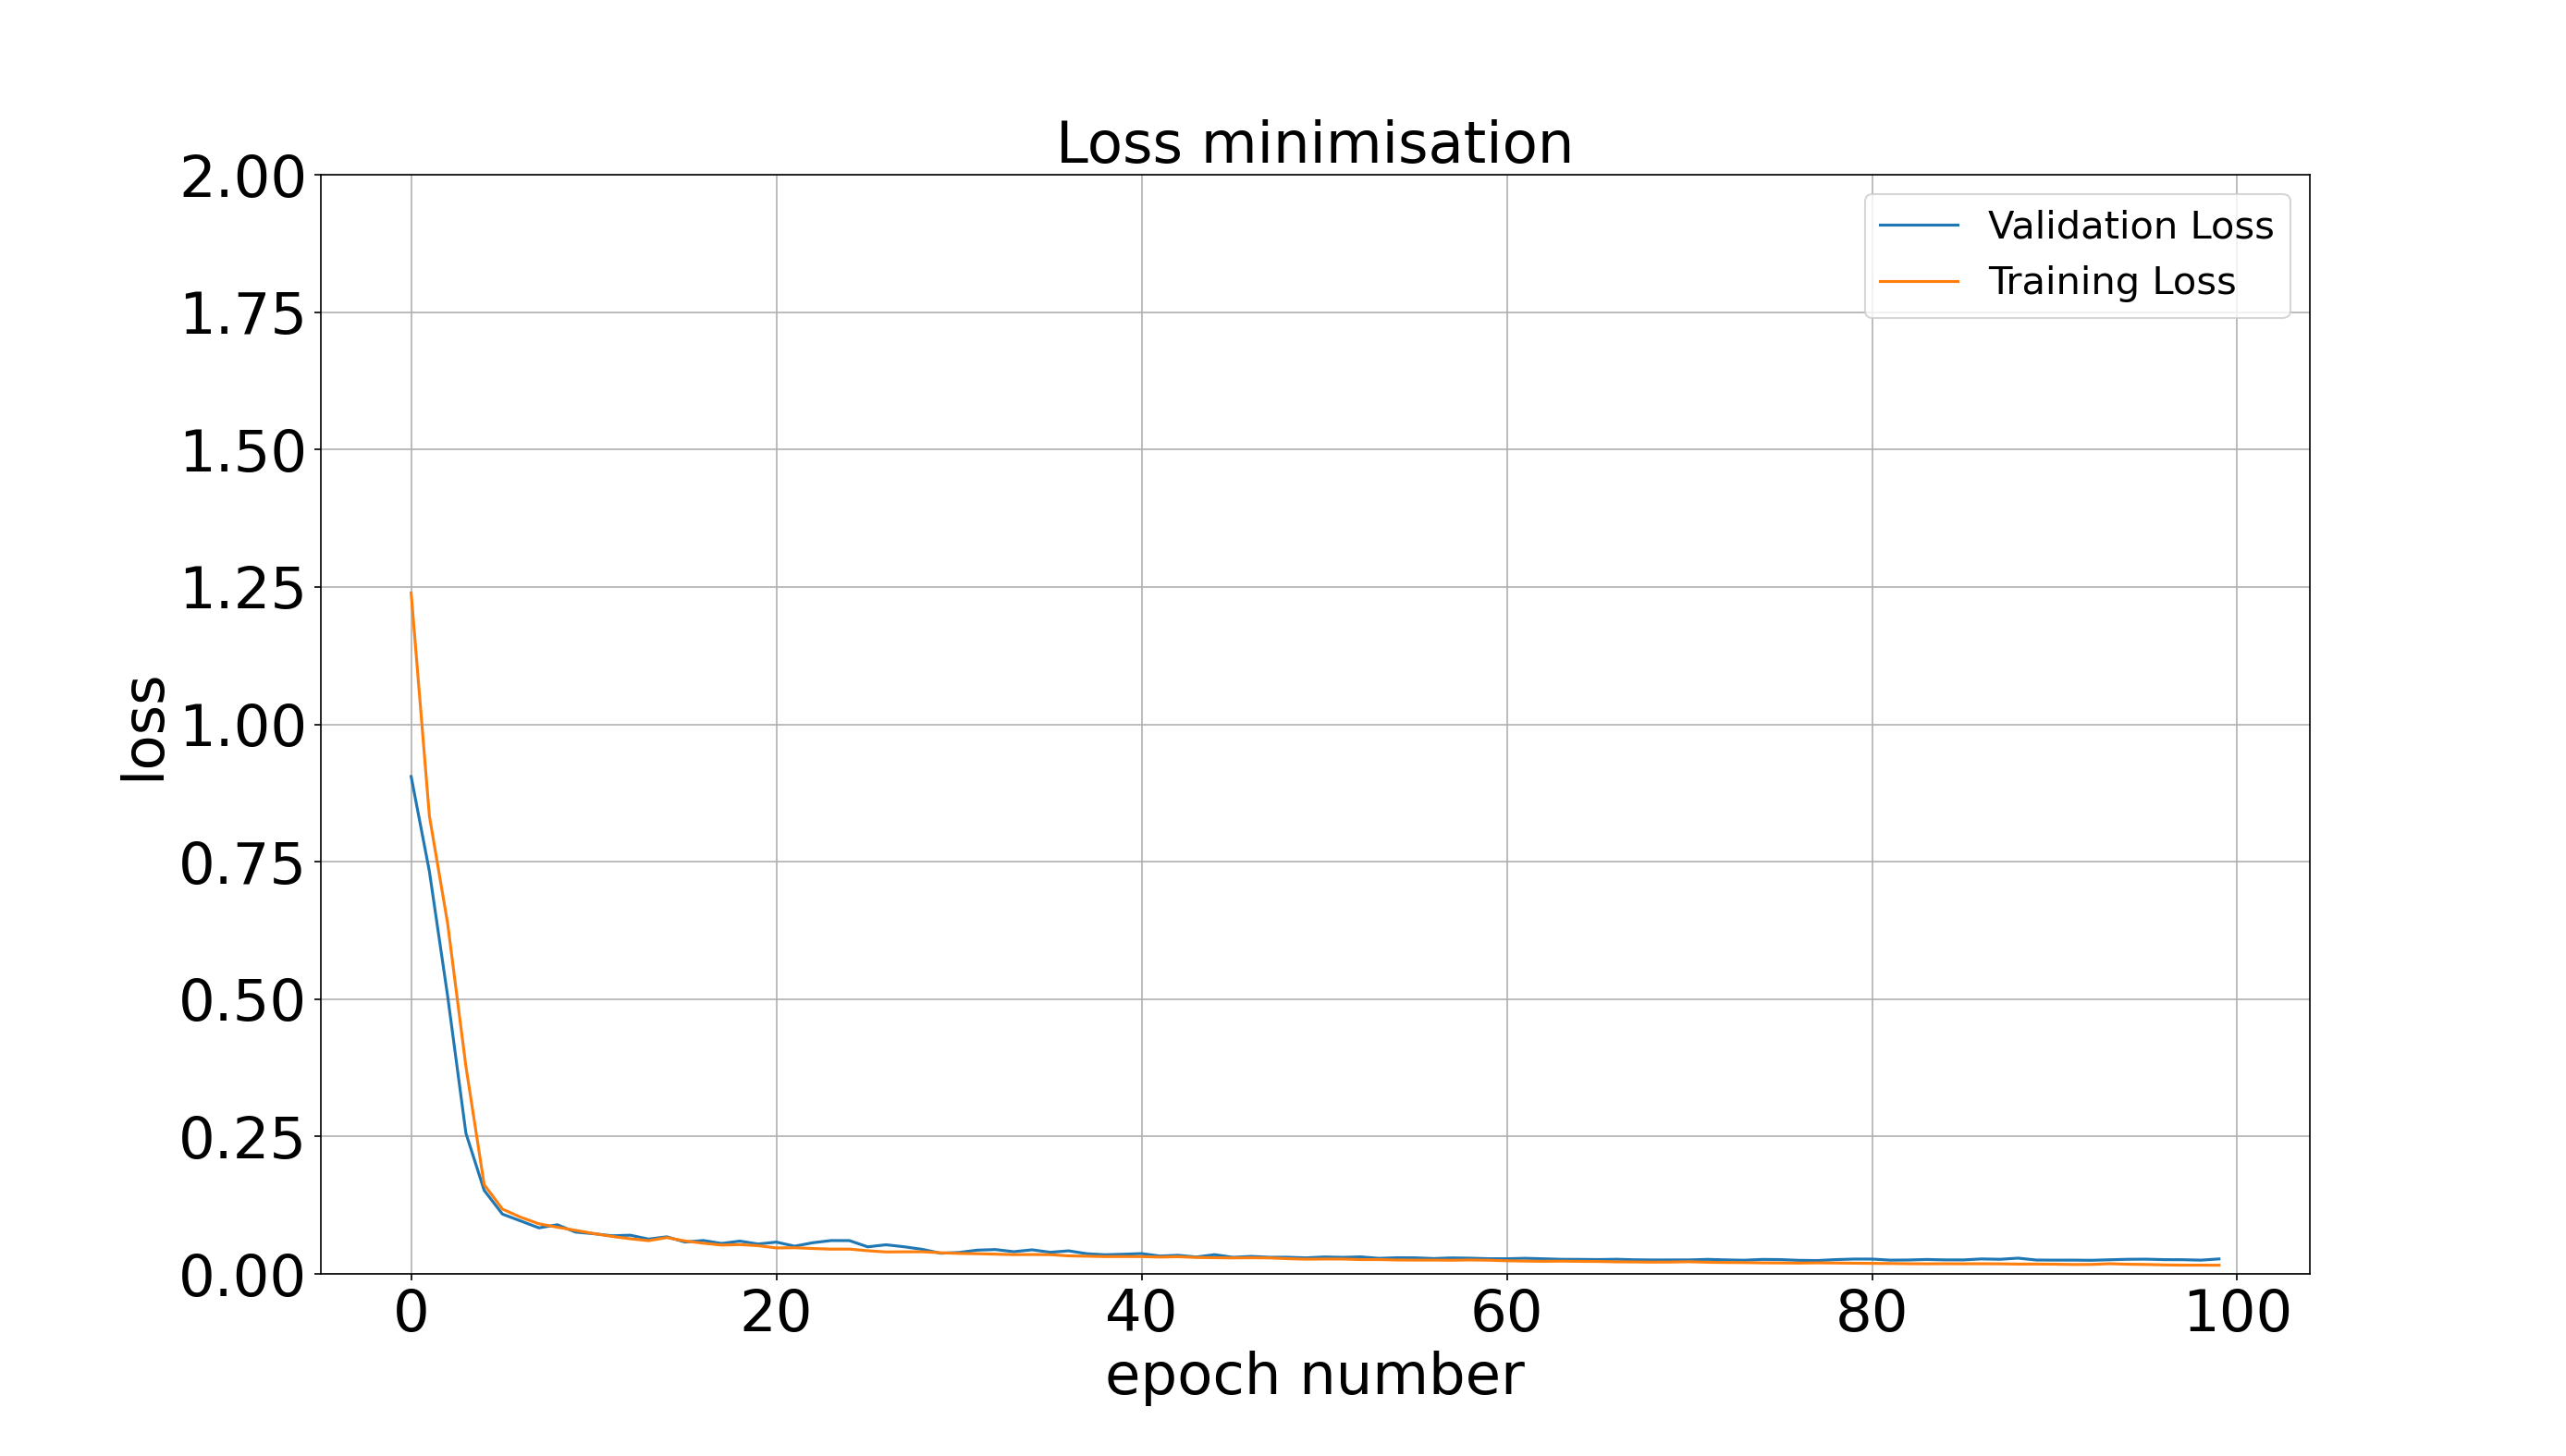
\includegraphics[ width=0.85\textwidth]{./images/results/modelB_loss_plot.png}
    \caption{Model B}
    \label{fig:loss_b}
   \end{subfigure}
   \caption{Loss function minimisation}
   \label{fig:modelloss}
\end{figure}

Aiming to analyse the robustness of our results, a set of statistical scores and tests were calculated. The pixel detailed information on the predictions allowed us to locate the tissue boundaries ILM, BM and CSI. Using this information we calculated the retinal and choroidal thickness for both the ground truth annotations and their predictions. Calculating both tissue layer's thickness allows us to compare further the resulting error find the degree of confidence of both models. The outcome of these tests are described in table \ref{tab:statistical_tests}.
\begin{table}[H]
    \begin{tabular}{l c|c|c|c|c}
         \textbf{Model} &\textbf{Layer} & \textbf{Test}& \textbf{P-value}  \\
         \hline
         A & Retina & Mann-Whitney U-Test & 3.14e-5 \\
         A & Choroid & Mann-Withney U-Test & 0.6483 \\
         A & Retina & T-test & 1.25e-5 \\
         A & Choroid & T-test & 0.6567 \\
         B & Retina & Mann-Whitney U-Test & 0.1115 \\
         B & Choroid & Mann-Withney U-Test & 0.3797 \\
         B & Retina & T-test & 0.1009 \\
         B & Choroid & T-test & 0.4571
    \end{tabular}
    \caption{Statistical Tests}
    \label{tab:statistical_tests}
\end{table}

Collecting the error expressed in micrometers allows us to understand how far the predictions were from the truth. The result of this comparison can be found in table \ref{tab:Error_Scores}. The Mean Absolute Error (MAE) describes  that both models have an average error under 3.5 $\mu m$ for both layers. Root Mean Squared Error (RMSE) as opposed to the absolute version penalizes the extreme values, therefore the measurements observed in averaging the data were significantly larger and tell us that on average when our models make a mistake the error can be quite significant, specially for Model A (trained using image augmentation) and the Choroid compartment of Model B. However this was not an often case when observing the low mean MAE's measures.

\begin{table}[H]
    \begin{tabular}{l c|c|c|c|c}
         \textbf{Model} &\textbf{Layer} & \textbf{Score}& \textbf{Error($\mu m$)}  \\
         \hline
         A & Retina & Root Mean Squared Error &  8.5793 \\
         A & Choroid & Root Mean Squared Error & 25.4270 \\
         A & Retina & Mean Absolute Error & 2.8557 \\
         A & Choroid & Mean Absolute Error & 3.4331 \\
         B & Retina & Root Mean Squared Error & 2.2634 \\
         B & Choroid & Root Mean Squared Error & 14.5819 \\
         B & Retina & Mean Absolute Error & 1.0735 \\
         B & Choroid & Mean Absolute Error & 2.3225 \\
    \end{tabular}
    \caption{Statistical Error Scores}
    \label{tab:Error_Scores}
\end{table}

\begin{figure}[H]
\centering
\begin{subfigure}{1\textwidth}
  \centering
  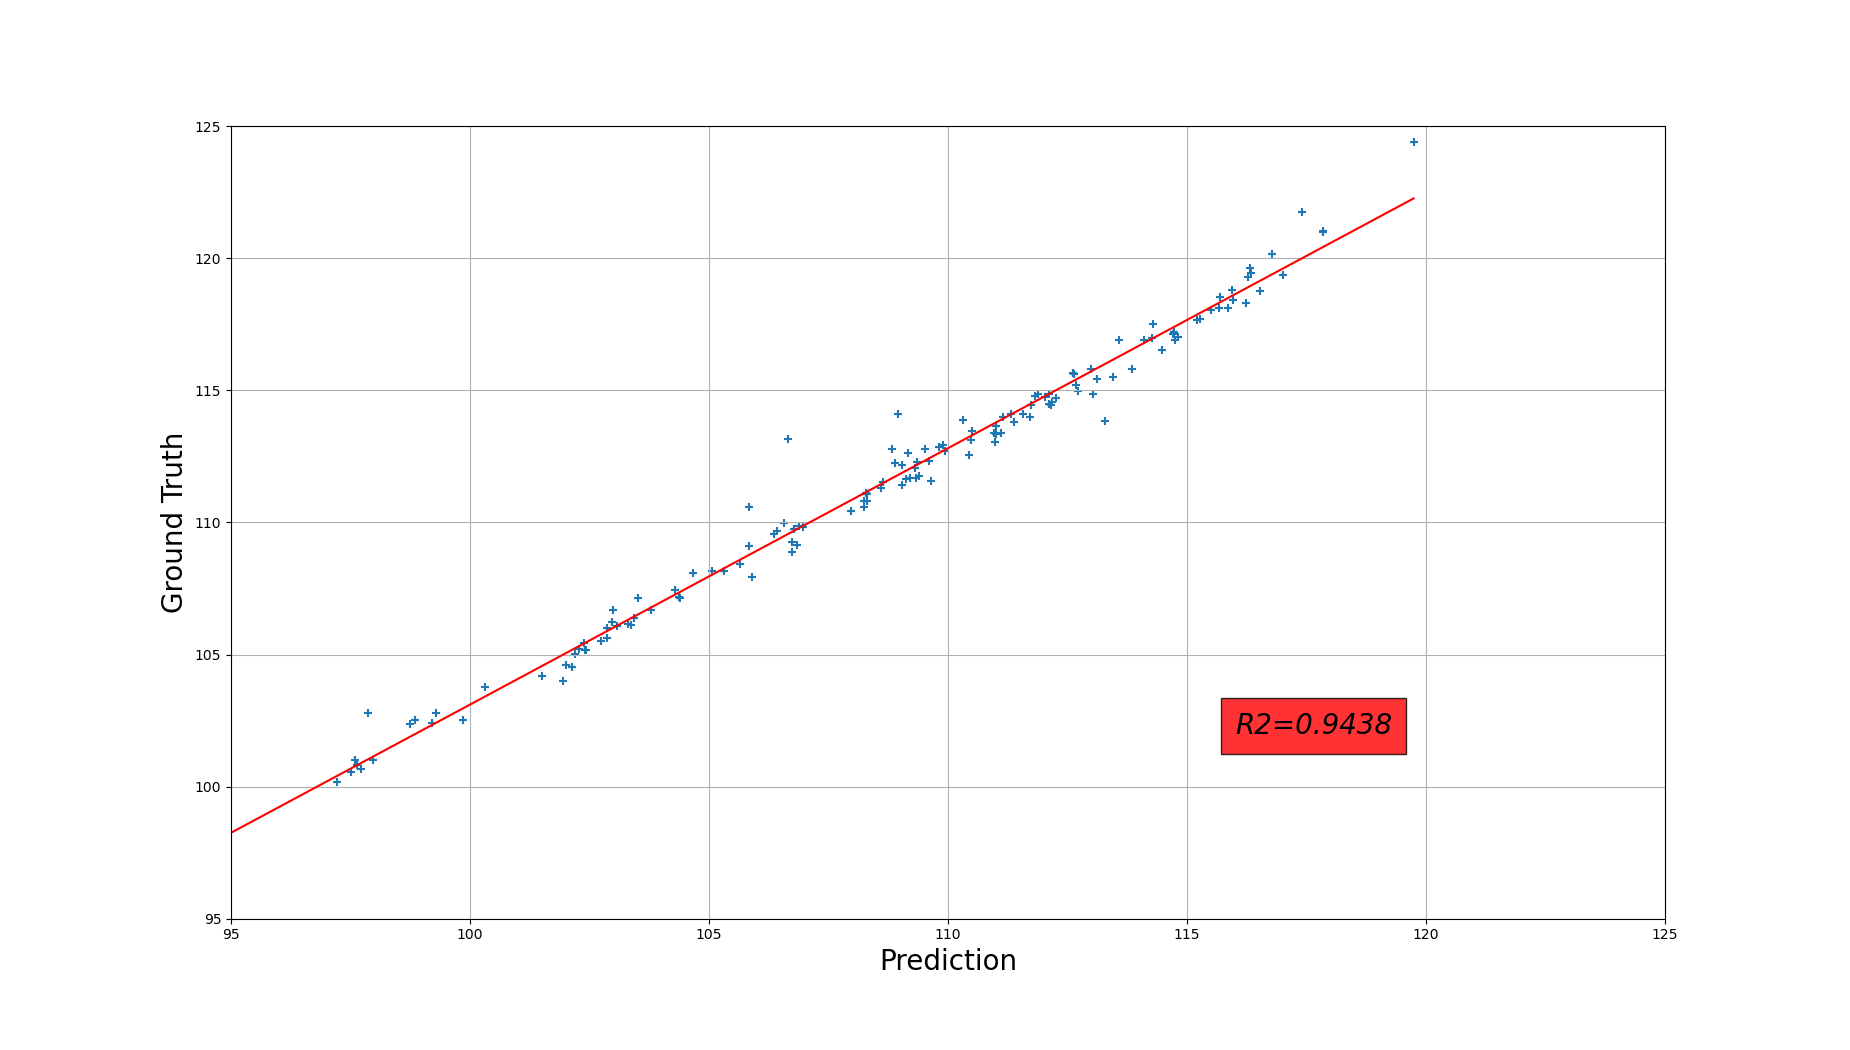
\includegraphics[width=\linewidth]{./results/model_A_retinal_thickness.png}
  \caption{Model A}
  \label{fig:model_a_specificity}
\end{subfigure}
\begin{subfigure}{1\textwidth}
  \centering
  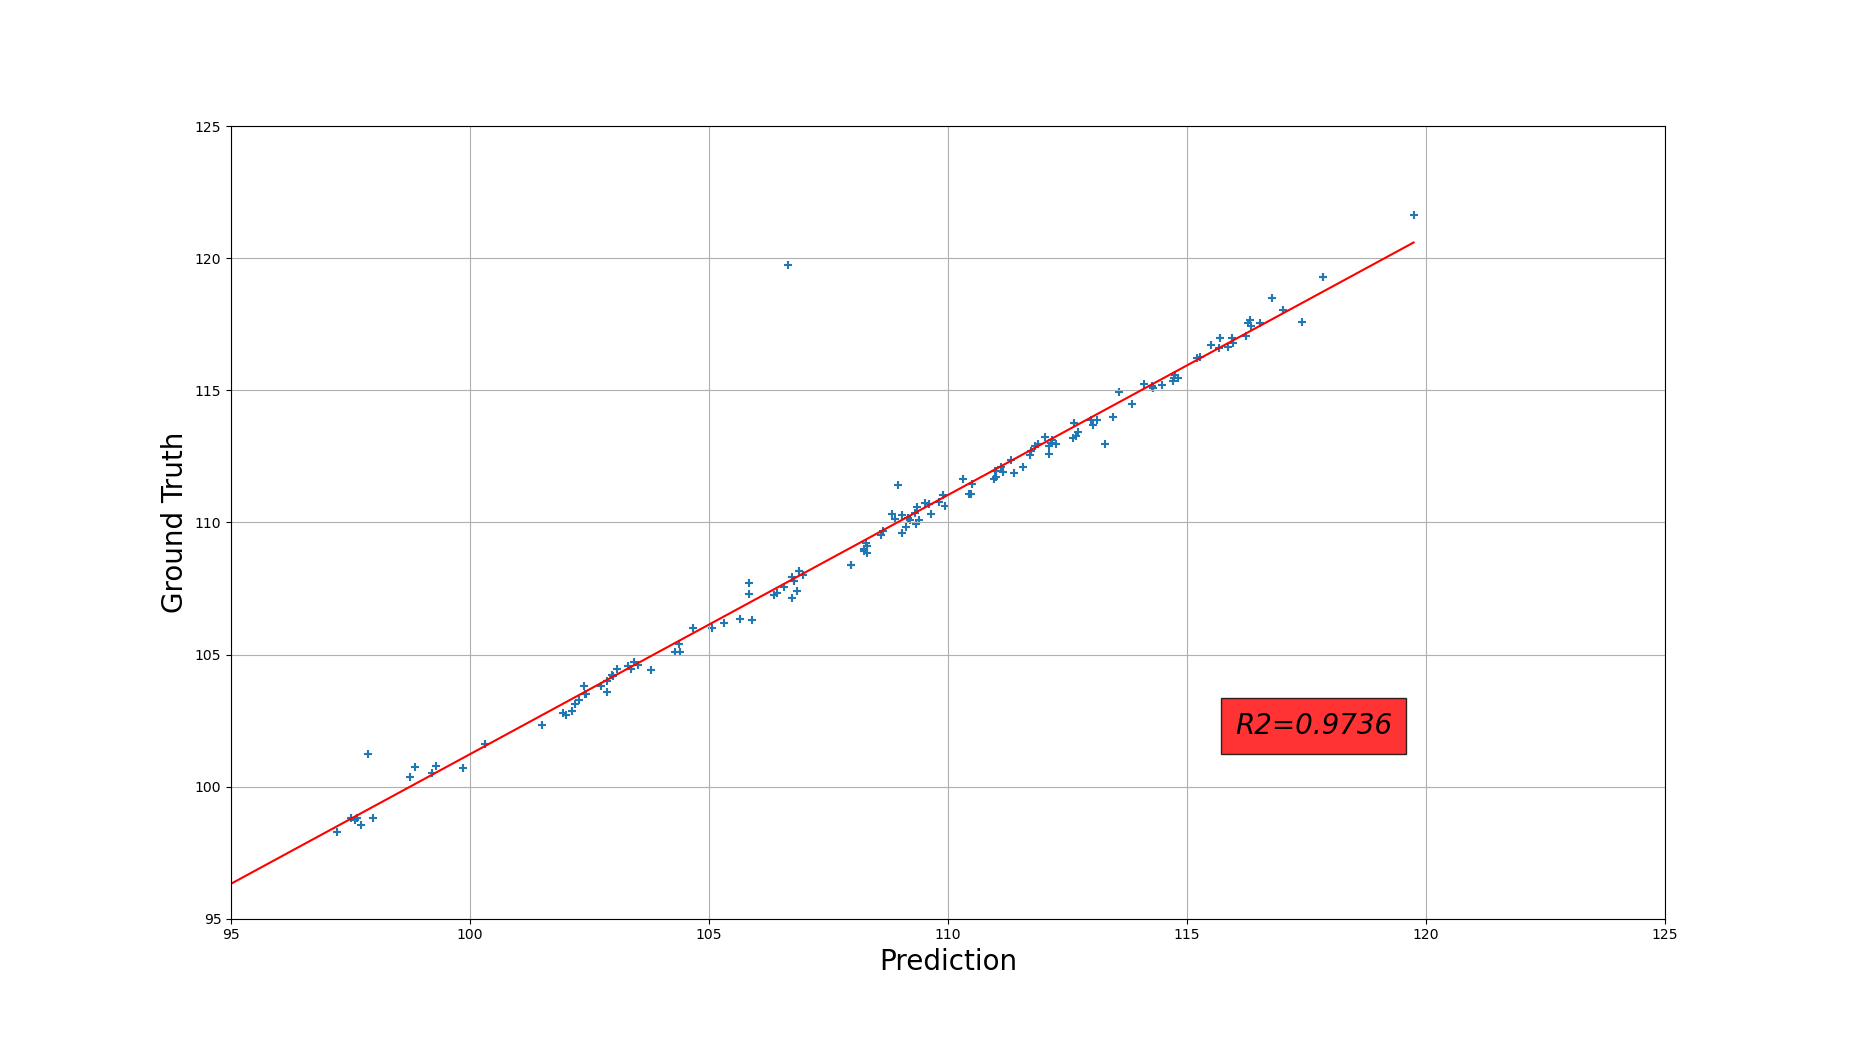
\includegraphics[width=\linewidth]{./results/model_B_retinal_thickness.png}
  \caption{Model B}
  \label{fig:modelb_specificity}
\end{subfigure}
\caption{Retinal Thickness Measures ($\mu m$)}
\label{fig:specificity_results}
\end{figure}

\begin{figure}[H]
\centering
\begin{subfigure}{1\textwidth}
  \centering
  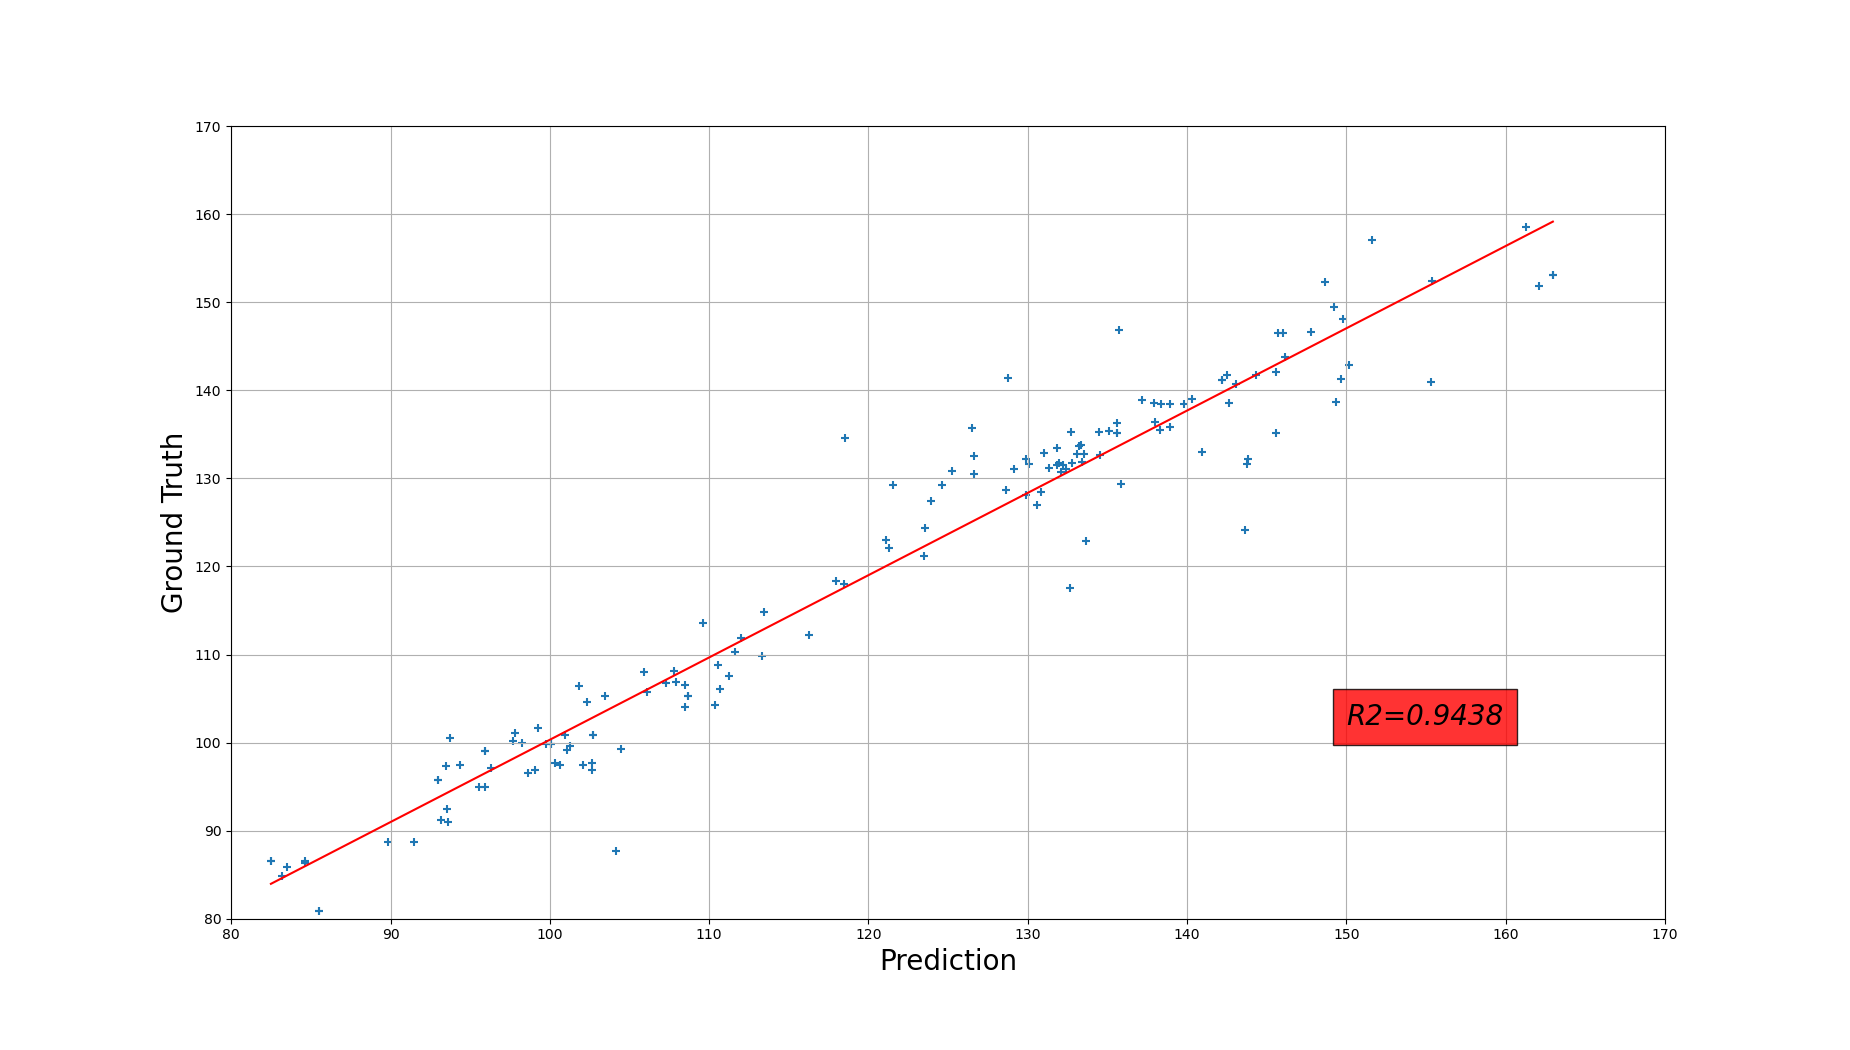
\includegraphics[width=\linewidth]{./results/model_A_choroidal_thickness.png}
  \caption{Model A}
  \label{fig:model_a_specificity}
\end{subfigure}
\begin{subfigure}{1\textwidth}
  \centering
  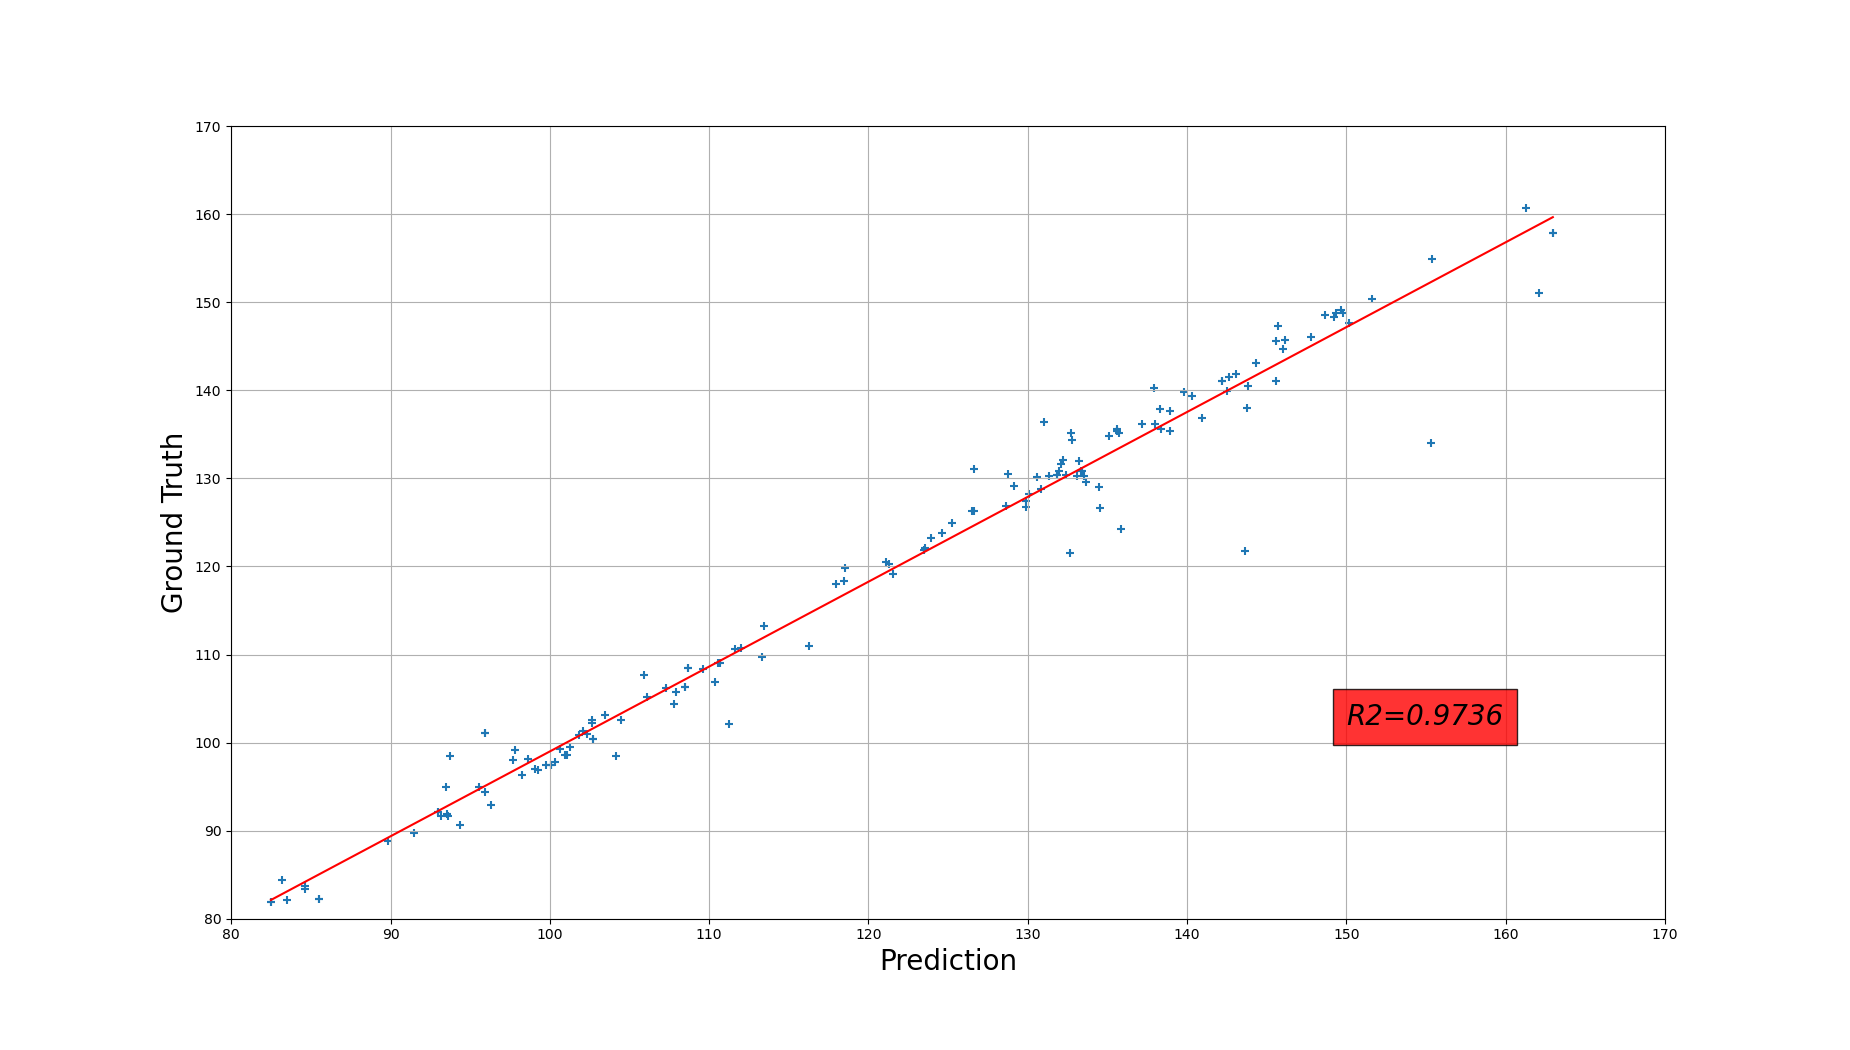
\includegraphics[width=\linewidth]{./results/model_B_choroidal_thickness.png}
  \caption{Model B}
  \label{fig:modelb_specificity}
\end{subfigure}
\caption{Choroidal Thickness Measures ($\mu m$)}
\label{fig:specificity_results}
\end{figure}

These results validate and indicate that an automated generation of synthetic ground truth for ophthalmic medical image analysis is technically feasible and produces segmentation maps similar to those of an expert ophthalmologist. 

\section{Conclusion}

Analysing the results of Model A and Model B we conclude that there is a high influence of image augmentation in the training of CNNs. Model B was trained during 100 epochs with a limited non-augmented dataset and it was able to learn better the features of the scans presenting a better Jaccard index than model A trained with augmentation (98,01\% vs 96,78\% respectively). Image Augmentation in this case is used to generate realistic transformations that can help the model to detect important features and to generalize the prediction on other type of OCT data even if in this case the evaluation measure takes a toll product of the randomness and number of augmented images. Model B also has a higher degree of sampling bias since the amount of images is relatively low and the distribution of features might not be representative enough to detect certain kind of characteristics present in other OCT scans either made with other devices or performed on different ethnic groups. Generally, sampling bias cannot be solved by artificially augmenting the images since the model only is able to learn from one type of population. In this case, machine learning engineers and healthcare professionals that use such a ML system need to be aware of what data was used to train the model and the influence that these can have in the results in relation with the target population that they address.


The influence of the inter and intra observer variability seen among experts when annotating data \cite{Maloca2019, Maloca2021, Ronchetti2019} may lead to 
influence of operator bias in the outputs of the model \cite{Gabr2016}. The problem arises from the reliance of supervised machine learning in the ground truth to learn the features of in the training data. It is expected that our model is highly biased towards the selected experts' agreement on what features on OCT scans define the position of the different boundaries used to separate the layers. Unfortunately, this can have a great impact on the final results since the model can only perform as accurately as the ground truth provided. 

From a medical perspective having an automated system that segments the 4 compartments present in an OCT scan means saving time invested in manually segmenting each B-scan. These time could be dedicated to enhance the care of the patient. However, since an operator bias is present in the outputs of the models, ML engineers need to ensure that training is performed using data following high standards of quality regarding the accuracy of the segmentations.

All in all, our framework is able to learn the features needed to accurately segment the OCT scans. However, it was noticed that artifacts introduced because of different conditions during the scanning process (brightness, eye position, band selection) can have a negative impact on the learning process, therefore, we could expect that raising the quality of the scans will lead to first a lower inter and intra observer variability and second a higher Jaccard coefficient which results on more accurate outputs.



\section{Future Work}

Further research into the topic would include dedicating significant resources to create a more representative dataset which would include OCT scans from different populations in order for the model to learn anatomical differences across different ethnic groups \cite{Consejo2020, Lin2009}. On the other hand, methods for accurately detecting the real position of every layer need to be implemented in order to avoid as much as possible the operator bias and interobserver variability. A suggested methodology might be to perform OCT scans on postmortem human eyes, manually annotate the segmentations from both the B-Scans and a posterior forensic analysis using a corresponding histopathology \cite{IOVINO2017, Mcnabb2009, Nioi2019} and correlate the data sources. Adding samples using this approach to our current dataset could improve the model learning process by avoiding the errors created by the presence of optical artifacts in the OCT scans resulting in more accurate ground truth. It would be expected that by having a clearer image, the inter and intra expert variability is minimal. This would help the model to identify features on boundaries that were missed in the current project as a result of the operator bias.

In order to improve the model outputs' Jaccard's coefficient, other ML models shall be implemented. Particularly implementing residual functions (Resnet model) might be beneficial for the overall performance as referred in \cite{He2015, Zheng2020}. The implementation could as well benefit from applying statistical rigourosity with techniques like variance analysis and p-tests and intragrader or intramodel comparisons. 

Finally, stacking up a series of automatically segmented B-scans to obtain a C-scan would allow us to output volumetric measures that would directly allow ophtalmologists to come up with choroidal and retinal thickness avoiding the manual annotation process of each B-Scan generated by the OCT spectrometer. 


\markboth{}{}

\newpage

\bibliographystyle{plain} % We choose the "plain" reference style
\bibliography{bibli} % Entries are in the "bibi.bib" file


\newpage

\markboth{}{}
  \normalsize
\begin{center}
\huge{\textbf{ Declaration of Independence}}\\[40mm]
\end{center}
\large
We confirm that the above work has been produced by the authors without any unauthorized assistance and without the use of any other means than those indicated, and that I have marked as such all passages that have been taken literally or meaningfully from published or unpublished writings.\\[30mm]
Bienne, the \today \\[10mm]
Emeline Lieberherr, Rayner Oswaldo Zorrilla Alfonzo
\begin{figure}[H]
    
\includegraphics[width=0.5\textwidth]{./images/signatures.png}
\end{figure}

\newpage
\appendix
\section*{Appendices}
\addcontentsline{toc}{section}{Appendices}
\renewcommand{\thesubsection}{\Alph{subsection}}

\subsection{Project Architecture Diagram}

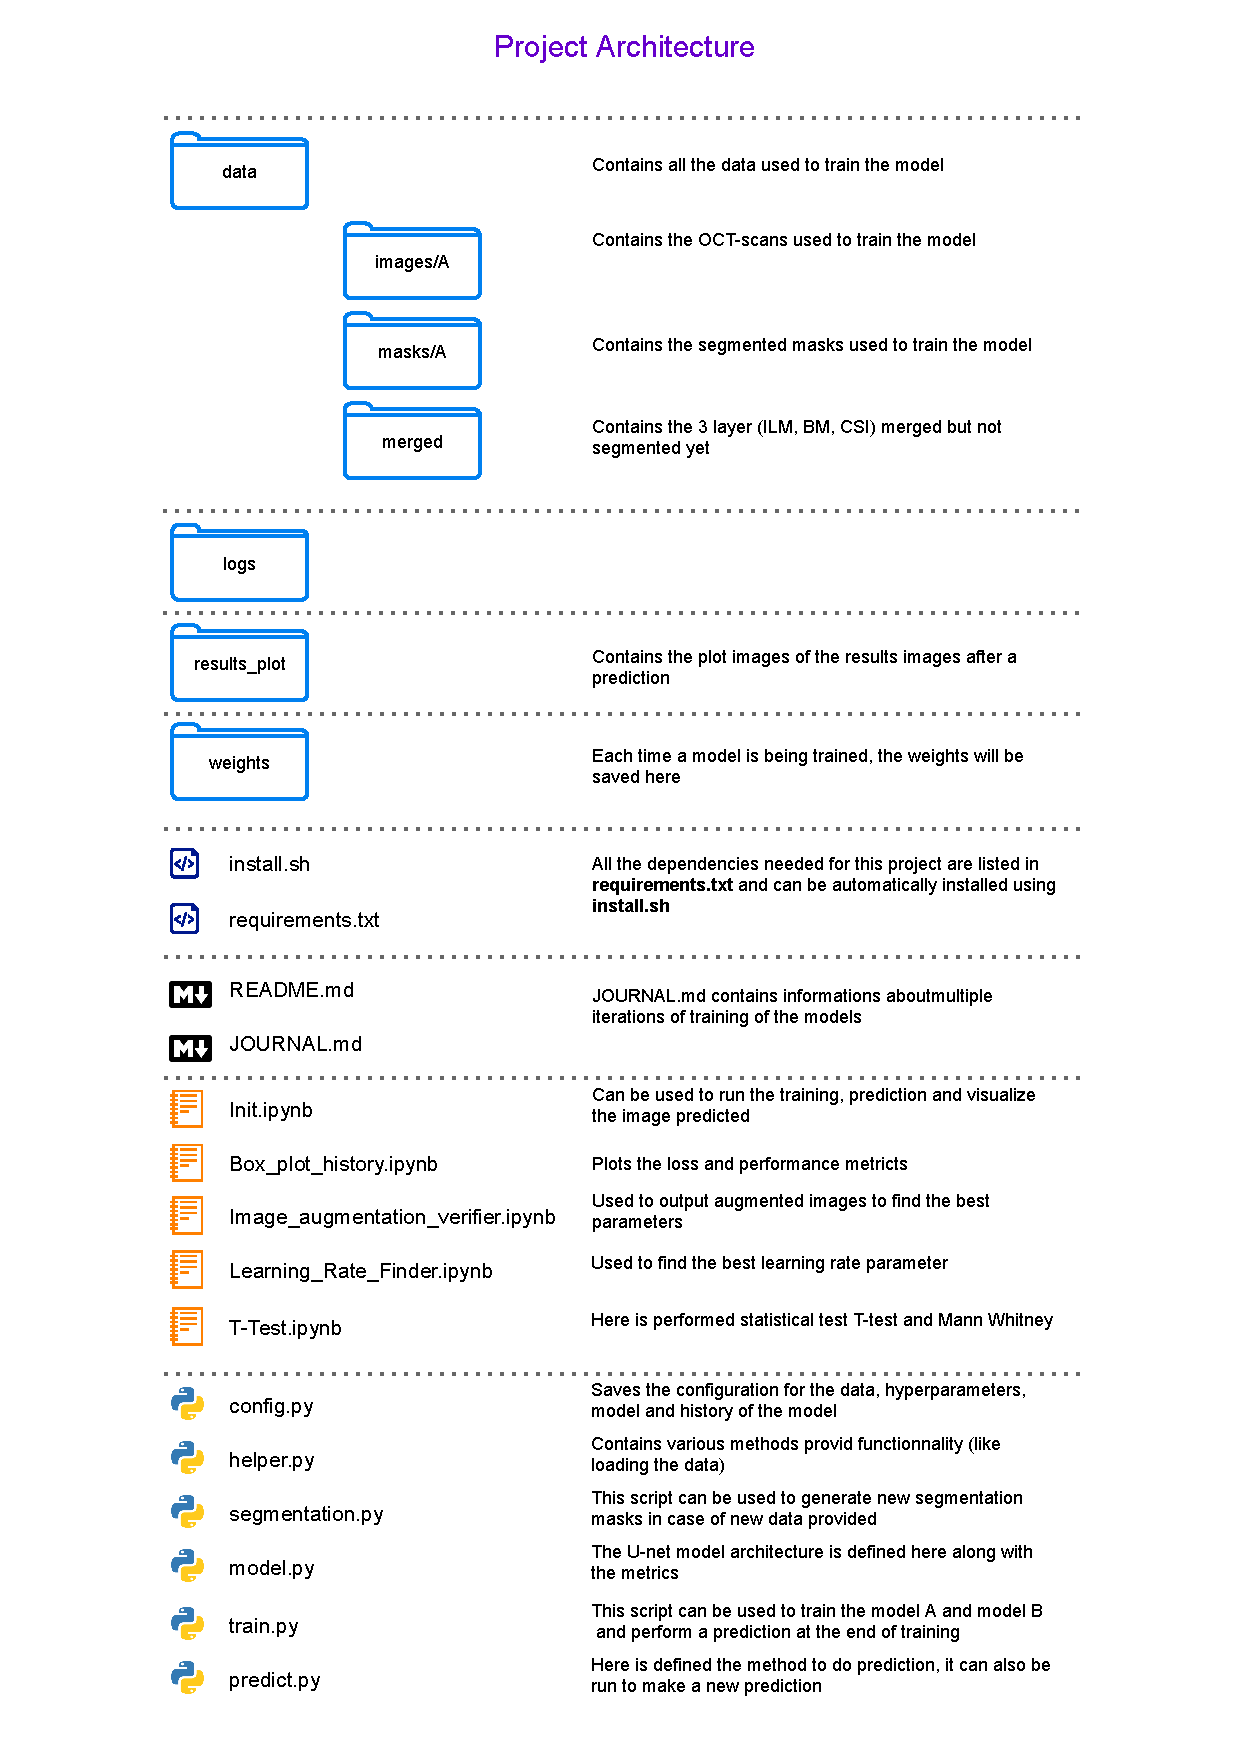
\includepdf[pages={1}]{./doc/appendix/projectArchitecture.pdf}
\subsection{Planning of Work and Tasks for the Project}
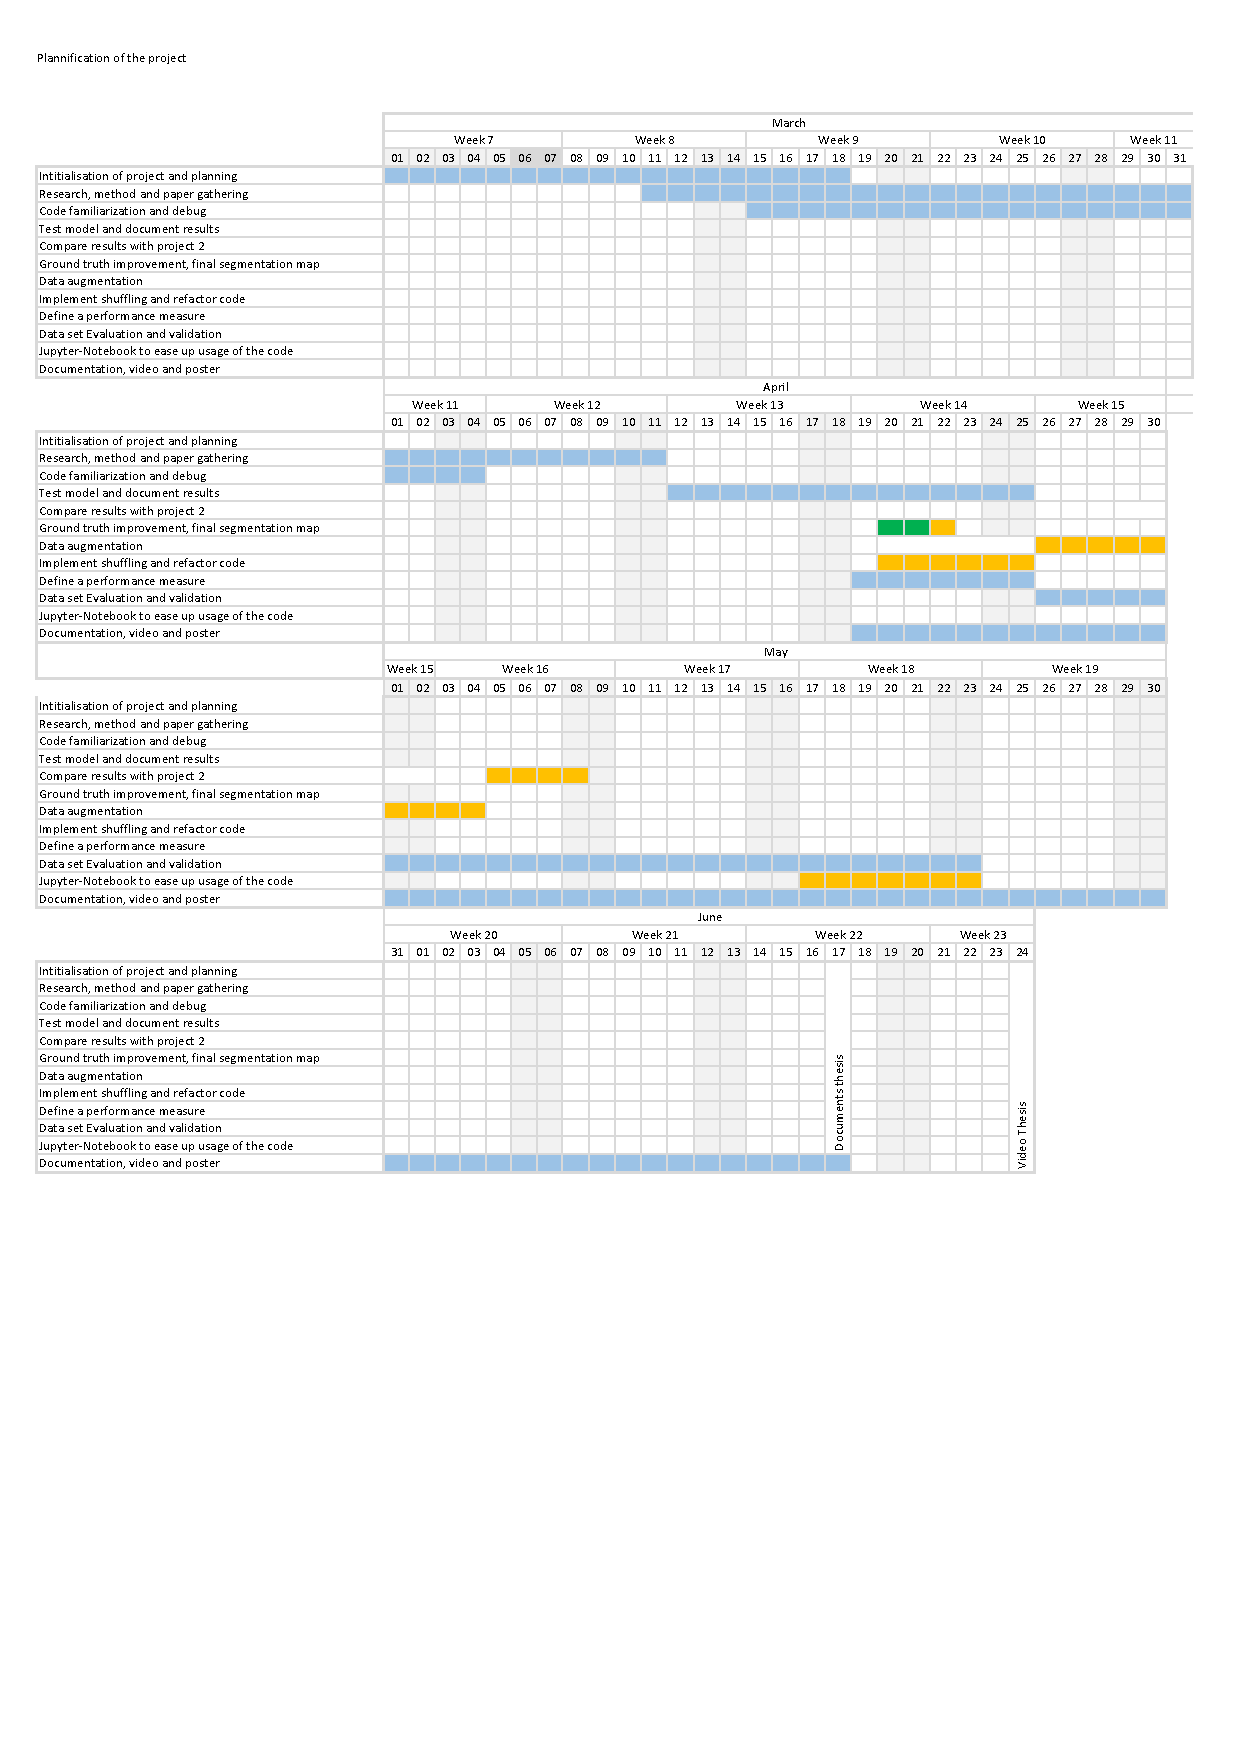
\includepdf[pages={1}]{./doc/appendix/plannification.pdf}

\end{document}